    \documentclass[runningheads]{llncs}
    
    % ---------------------------------------------------------------
    % Include basic ECCV package
  
    % TODO REVIEW: Insert your submission number below by replacing '*****'
    % TODO FINAL: Comment out the following line for the camera-ready version
    \usepackage{microtype}
    \usepackage[review,year=2026,ID=3192]{eccv}
    % TODO FINAL: Un-comment the following line for the camera-ready version
    %\usepackage{eccv}
    
    % OPTIONAL: Un-comment the following line for a version which is easier to read
    % on small portrait-orientation screens (e.g., mobile phones, or beside other windows)
    %\usepackage[mobile]{eccv}
    \usepackage{multirow}
    \usepackage[table]{xcolor}
    \usepackage{appendix}
    \usepackage{amssymb}       % 符号支持
    \usepackage{pifont}
    \usepackage{makecell} % 用于单元格换行

    \usepackage{adjustbox} % 用于精细控制
    \usepackage{caption}

 
    % ---------------------------------------------------------------
    % Other packages
    
    % Commonly used abbreviations (\eg, \ie, \etc, \cf, \etal, etc.)
    \usepackage{eccvabbrv}
    
    % Include other packages here, before hyperref.
    \usepackage{graphicx}
    \usepackage{booktabs}
    
    % The "axessiblity" package can be found at: https://ctan.org/pkg/axessibility?lang=en
    \usepackage[accsupp]{axessibility}  % Improves PDF readability for those with disabilities.
    
    
    % ---------------------------------------------------------------
    % Hyperref package
    
    % It is strongly recommended to use hyperref, especially for the review version.
    % Please disable hyperref *only* if you encounter grave issues.
    % hyperref with option pagebackref eases the reviewers' job, but should be disabled for the final version.
    %
    % If you comment hyperref and then uncomment it, you should delete
    % main.aux before re-running LaTeX.
    % (Or just hit 'q' on the first LaTeX run, let it finish, and you
    %  should be clear).
    
    % TODO FINAL: Comment out the following line for the camera-ready version
    %\usepackage[pagebackref,breaklinks,colorlinks,citecolor=eccvblue]{hyperref}
    % TODO FINAL: Un-comment the following line for the camera-ready version
    \usepackage{hyperref}
    \usepackage{wrapfig}
    % Support for ORCID icon
    \usepackage{orcidlink}
    % 美化
    \usepackage{xcolor}
    \usepackage{pifont}

    \definecolor{firstpurple}{RGB}{240, 235, 255}  % 第一名
    \definecolor{secondpurple}{RGB}{248, 245, 255} % 第二名
    % 定义带颜色的勾和叉
    \newcommand{\cmark}{\textcolor{blue}{\ding{51}}}
    \newcommand{\xmark}{\textcolor{red}{\ding{55}}}
    
    \begin{document}
    
    % ---------------------------------------------------------------
    \title{RoboStream: Weaving \underline{S}patio-\underline{T}emporal \underline{Rea}soning with \underline{M}emory 
    in Vision-Language Models for \underline{Robo}tics}
    
    % TODO REVIEW: If the paper title is too long for the running head, you can set
    % an abbreviated paper title here. If not, comment out.
    \titlerunning{RoboStream}
    
    % TODO FINAL: Replace with your author list. 
    % Include the authors' OCRID for the camera-ready version, if at all possible.
    \author{First Author\inst{1}\orcidlink{0000-1111-2222-3333} \and
    Second Author\inst{2,3}\orcidlink{1111-2222-3333-4444} \and
    Third Author\inst{3}\orcidlink{2222--3333-4444-5555}}
    
    % TODO FINAL: Replace with an abbreviated list of authors.
    \authorrunning{F.~Author et al.}
    % First names are abbreviated in the running head.
    % If there are more than two authors, 'et al.' is used.
    
    % TODO FINAL: Replace with your institution list.
    \institute{Princeton University, Princeton NJ 08544, USA \and
    Springer Heidelberg, Tiergartenstr.~17, 69121 Heidelberg, Germany
    \email{lncs@springer.com}\\
    \url{http://www.springer.com/gp/computer-science/lncs} \and
    ABC Institute, Rupert-Karls-University Heidelberg, Heidelberg, Germany\\
    \email{\{abc,lncs\}@uni-heidelberg.de}}
    
    \maketitle
    


\begin{abstract}
Enabling reliable long-horizon robotic manipulation is a crucial step toward open-world embodied intelligence. However, VLM-based planners treat each step as an isolated observation-to-action mapping, forcing them to reinfer scene geometry from raw pixels at every decision step while remaining unaware of how prior actions have reshaped the environment. Despite strong short-horizon performance, these systems lack the spatio-temporal reasoning required for persistent geometric anchoring and memory of action-triggered state transitions. Without persistent state tracking, perceptual errors accumulate across the execution horizon, temporarily occluded objects are catastrophically forgotten, and these compounding failures lead to precondition violations that cascade through subsequent steps. In contrast, humans maintain a persistent mental model that continuously tracks spatial relations and action consequences across interactions rather than reconstructing them at each instant.
Inspired by this human capacity for causal spatio-temporal reasoning with persistent memory, we propose \textbf{RoboStream}, a training-free framework that achieves geometric anchoring through Spatio-Temporal Fusion Tokens (STF-Tokens), which bind visual evidence to 3D geometric attributes for persistent object grounding, and maintains causal continuity via a Causal Spatio-Temporal Graph (CSTG) that records action-triggered state transitions across steps. This design enables the planner to trace causal chains and preserve object permanence under occlusion without additional training or fine-tuning. RoboStream achieves 90.5\% on long-horizon RLBench and 44.4\% on challenging real-world block-building tasks, where both SoFar and VoxPoser score 11.1\%, demonstrating that spatio-temporal reasoning and causal memory are critical missing components for reliable long-horizon manipulation.








\keywords{Robot Manipulation \and Vision-Language Models \and Long-Horizon Planning \and Spatio-Temporal Reasoning \and Causal Memory}
\end{abstract}
    

% \section{Introduction}
\label{sec:intro}

Vision-language models (VLMs) have emerged as powerful planners for robotic manipulation, leveraging internet-scale semantic knowledge and visual perception to translate high-level instructions into executable action sequences~\cite{zitkovich2023rt, kim2025openvla, driess2023palm, jiang2023vima}. VLM-based systems have demonstrated strong performance on short-horizon manipulation tasks, including precise grasping, pose-aware placement, and decomposition of language instructions into subgoal sequences~\cite{brohan2023saycan, qisofar, huang2023voxposer, shridhar2023perceiver}.

However, this success does not readily extend to long-horizon tasks, which demand sustained spatial and causal awareness across multi-step action sequences that irreversibly alter the environment~\cite{shi2025hi, zhao2025cot, wu2023tidybot}. Current VLM-based planners lack the persistent state tracking required to bridge observations across steps, forcing them to reinfer world state from partial observations at each decision step~\cite{hanrobocerebra, huang2023inner, zhou2025code}. Without accumulated context, perceptual errors and action effects compound across steps, ultimately resulting in cascading failures, as illustrated in Fig.~\ref{fig:teaser}. In contrast, humans maintain a coherent mental model~\cite{lake2017building} that continuously integrates spatial relations and causal consequences as actions unfold, tracking not only where objects are but also how each action has cumulatively reshaped the world.



\begin{figure}[t]
        \centering  
        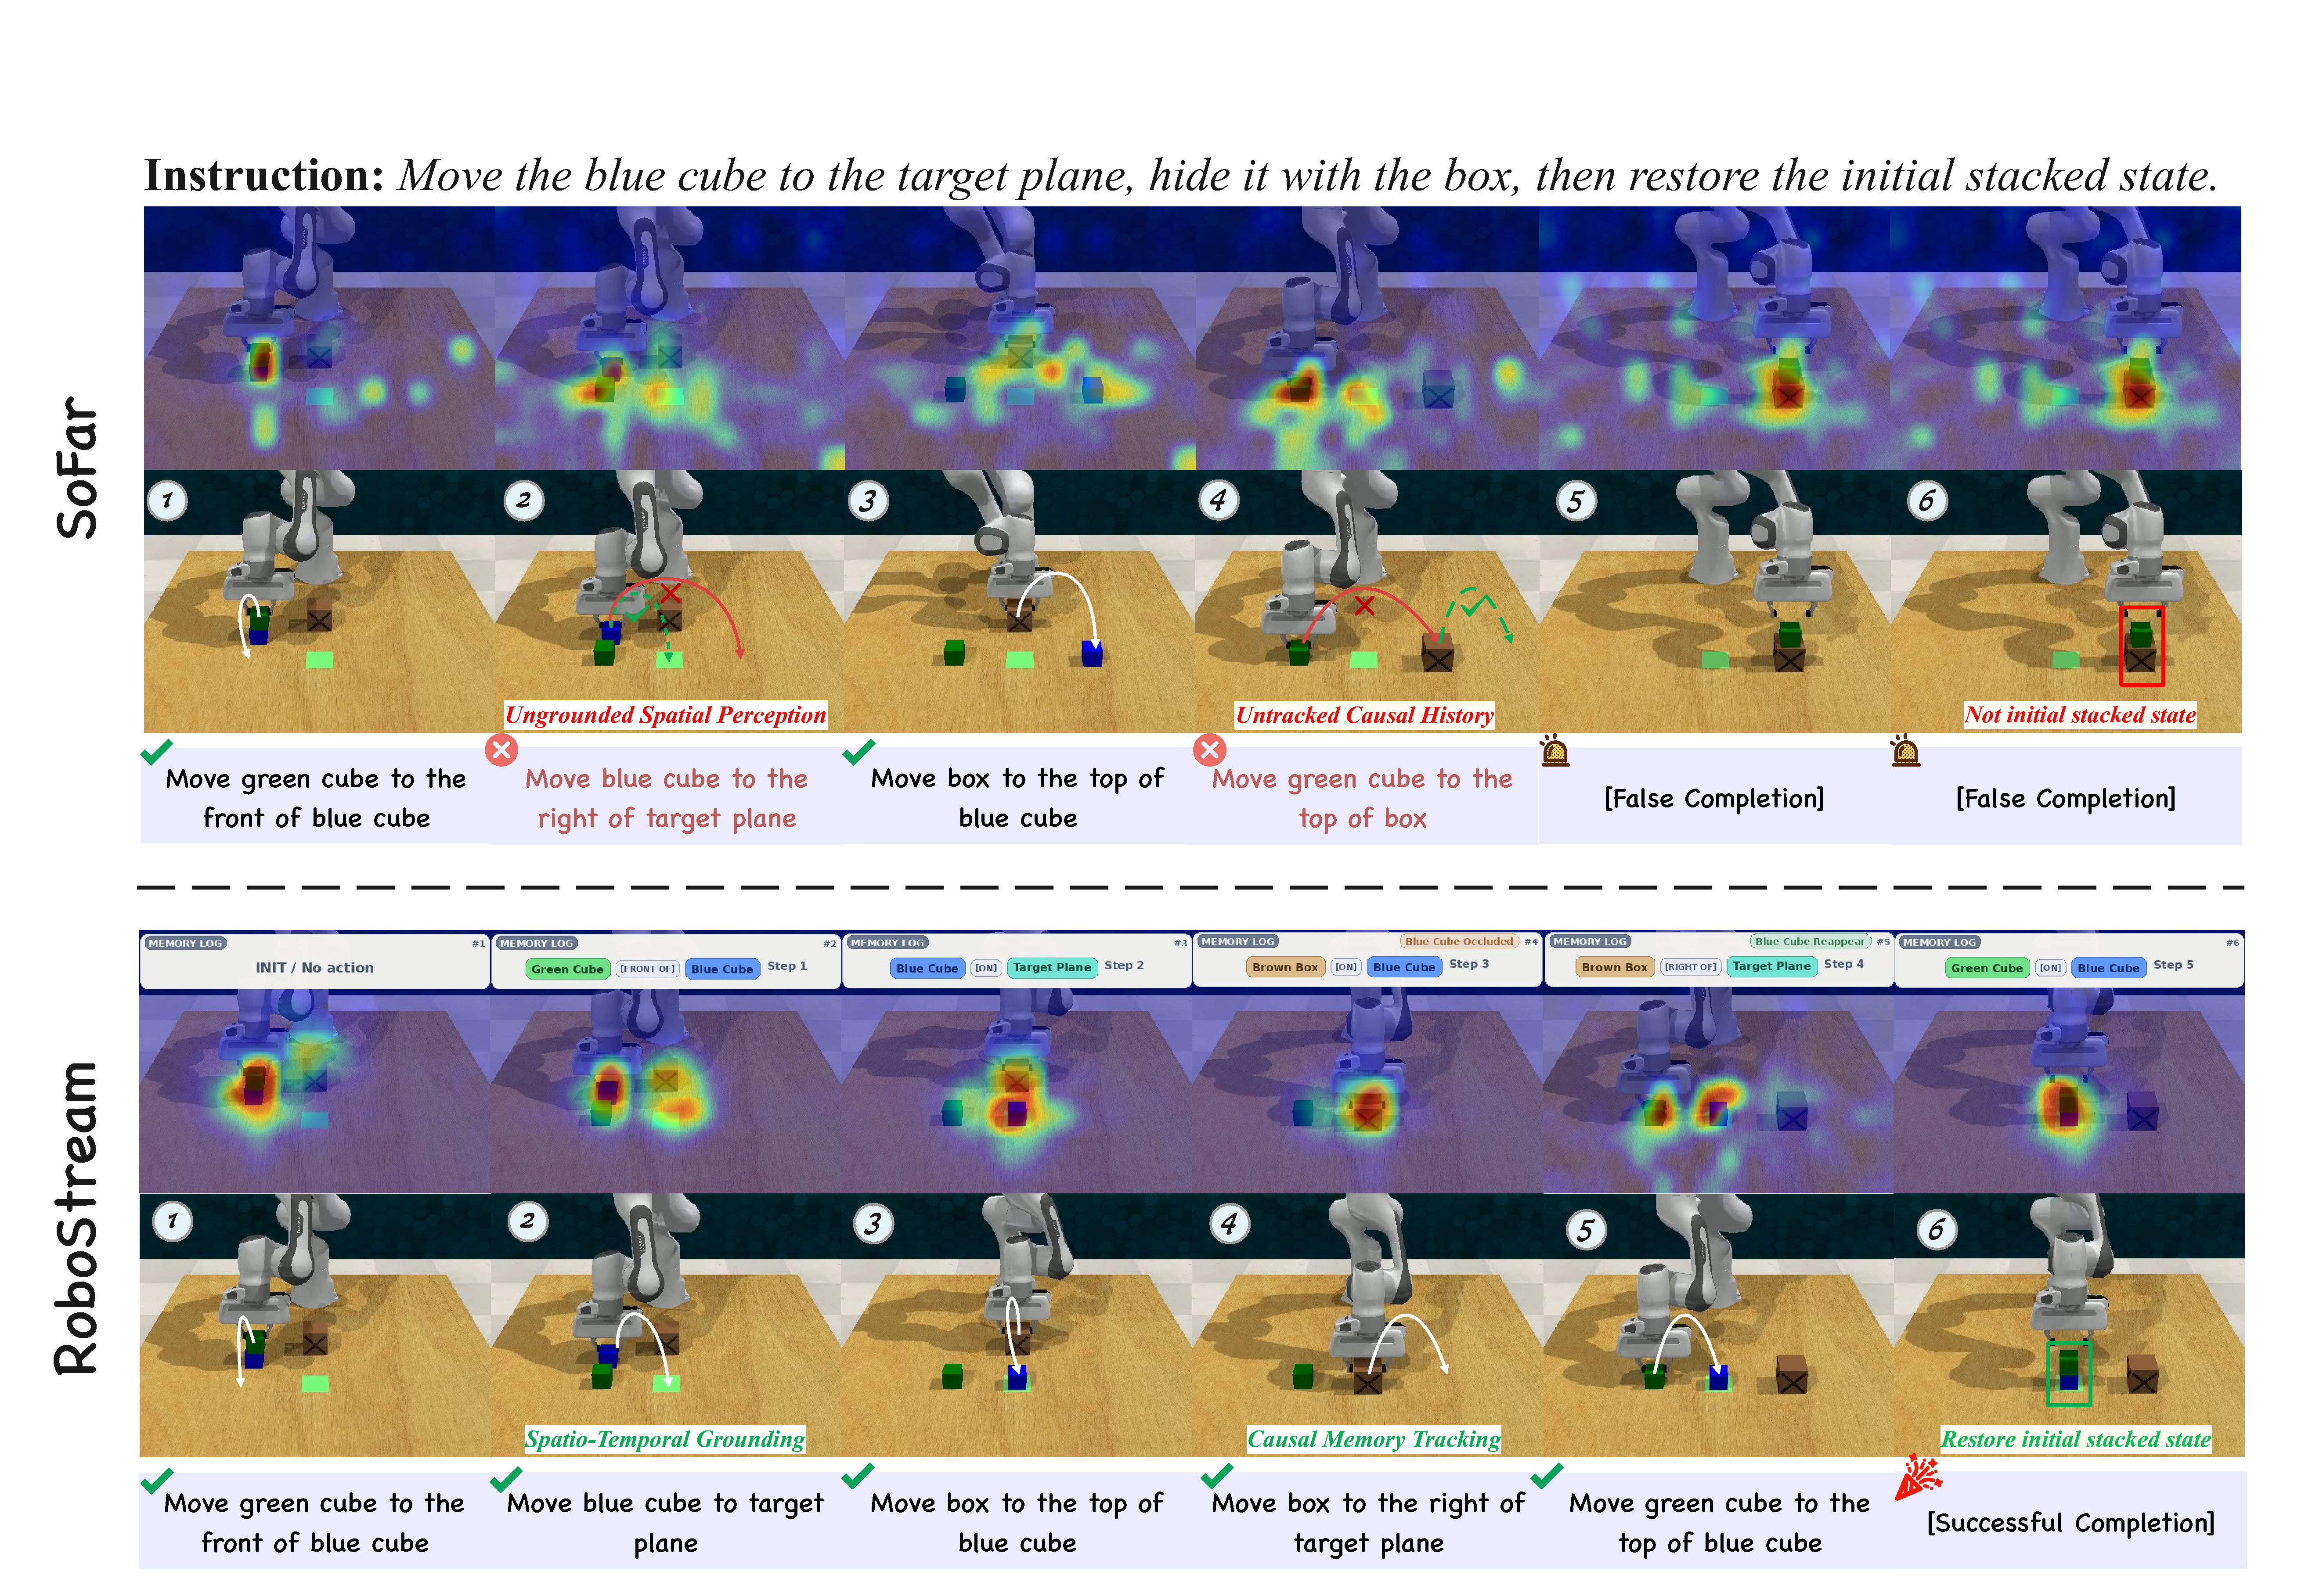
\includegraphics[width=1\textwidth]{Figures/RoboStream_Intro_Compare.pdf}
        \caption{\textbf{Qualitative comparison between SoFar~\cite{qisofar} and RoboStream.} This long-horizon task involves object occlusion and state restoration. \textbf{Top (SoFar):} Diffuse attention heatmaps and absent memory logs reveal two cascading failures: \textit{Ungrounded Spatial Perception} misplaces the blue cube at Step~2, while \textit{Untracked Causal History} leaves the planner unaware of the occluded cube at Step~4, resulting in an incorrect final state. \textbf{Bottom (RoboStream):} Concentrated attention heatmaps and persistent memory logs show that \textit{Spatio-Temporal Grounding} enables accurate object placement at Step~2, while \textit{Causal Memory Tracking} maintains awareness of the occluded cube at Step~4, enabling successful task completion.}
\label{fig:teaser}
\end{figure}


Replicating this human capacity for spatio-temporal reasoning requires persistent tracking of two interdependent quantities, namely the evolving geometric state of each object across steps and the causal record of how actions modify those states. Tracking alone is insufficient, as geometric states must be anchored in 3D space for reliable spatial reasoning while causal records must be structured to support inference over displaced or occluded objects. 
Current VLM-based planners fail at both, as illustrated in~Fig.~\ref{fig:teaser}, exposing two tightly coupled representation deficits.
\ding{172}~\textit{Ungrounded Spatial Perception}: spatial relations in manipulation are latent state components continually rewritten by contact and motion, yet current systems infer them implicitly via image-centric perception without geometric anchoring or cross-step identity binding~\cite{chen2024spatialvlm, huang2024copa, yuan2025robopoint}. This forces geometry reconstruction from raw pixels at every step, where small inaccuracies accumulate into spatial hallucinations and precondition violations.
\ding{173}~\textit{Untracked Causal History}: although actions irreversibly alter the environment, existing methods retain no record linking actions to induced state transitions. Without causal tracking, planners remain unaware of displaced objects and lose track of occluded ones entirely, leading to precondition violations when subsequent actions depend on altered states~\cite{wen2025dexvla, zhen20243d}.


To address these two deficits, we propose \textbf{RoboStream}, a training-free framework that weaves spatio-temporal reasoning and persistent memory directly into the VLM planning loop through \textit{Spatio-Temporal Grounding} and \textit{Causal Memory Tracking}. For grounding, Spatio-Temporal Fusion Tokens (STF-Tokens) distill visual appearance and 3D geometry (centroid and Gaussian shape) of each object into identity-persistent primitives, shifting VLM reasoning from pixel-level reconstruction to structured object-instance references that suppress cascading spatial errors. For tracking, a Causal Spatio-Temporal Graph (CSTG) records action-triggered state transitions alongside persistent object identities, preserving object permanence under occlusion without direct visual evidence.
We evaluate RoboStream on five benchmarks spanning simulated and real-world settings: SIMPLER~\cite{li2025evaluating}, long-horizon RLBench tasks~\cite{james2020rlbench}, 6-DoF SpatialBench~\cite{qisofar}, Open6DOR V2~\cite{ding2024open6dor}, and long-horizon real-world Franka experiments including block building, disassembly, and hide-and-restore under occlusion.
Across all settings, RoboStream outperforms existing VLM-based planners, demonstrating that spatio-temporal reasoning and persistent memory are essential for robust long-horizon manipulation.
Our contributions are as follows:

1) We introduce \textbf{RoboStream}, a training-free framework weaving spatio-te\-m\-p\-o\-r\-a\-l reasoning with persistent memory to overcome spatial hallucination and causal blindness in VLM-based planners. By anchoring geometric evidence across steps and tracking causal state transitions, RoboStream builds persistent world representations enabling robust long-horizon reasoning without retraining.


2) We design two synergistic mechanisms for Spatio-Temporal Grounding and Causal Memory Tracking. \textit{Spatio-Temporal Fusion Tokens (STF-Tokens)} bind visual evidence to 3D geometry, converting pixel-level inference into deterministic spatial references. A \textit{Causal Spatio-Temporal Graph (CSTG)} maintains object identities and records action-triggered state transitions, enabling causal inference of occluded states and preventing error accumulation over long horizons.

3) RoboStream achieves state-of-the-art results across five benchmarks spanning long-horizon manipulation (RLBench, real-world Franka), zero-shot generalization (SIMPLER), and spatial reasoning (6-DoF SpatialBench, Open6DOR V2), validating that weaving spatio-temporal reasoning with persistent memory is essential for robust manipulation across diverse settings.




% \section{Related Work}
\label{sec:related_work}

\subsection{Spatial Understanding with VLMs}
Spatial understanding underpins robotic manipulation by recovering geometric relationships. Approaches overcome VLM limitations through two main strategies.
Tool-augmented methods~\cite{ding2024open6dor, qin2025robofactory, zhudexflywheel, tan2025roboos} delegate VLMs to orchestrate external visual foundation models or geometric engines. SpaceTools~\cite{chen2025spacetools} combines dual-interaction reinforcement learning with geometric reasoning, while TIGER~\cite{han2025tiger} synthesizes code-based geometric routines. These externalize computation but add overhead and require module coupling.
3D-data-driven fine-tuning~\cite{cheng2024spatialrgpt, song2025robospatial, daxberger2025mm, raysat, wang2025spatial457} strengthens spatial representations through pseudo-3D or real-world 3D data. RoboRefer~\cite{zhouroborefer} integrates depth encoders, SpatialBot~\cite{cai2025spatialbot} applies progressive spatial curricula, and SpatialVLM~\cite{chen2024spatialvlm} leverages large-scale 3D spatial QA datasets. Fine-tuning incurs substantial data and training costs.
RoboStream contrasts by anchoring visual evidence directly to explicit 3D geometry via STF-Tokens, requiring no fine-tuning and maintaining persistent spatial representations across sequential steps without external modules or retraining.

\subsection{VLMs for Robotic Manipulation}
Robotic manipulation bridges semantic reasoning with execution along three complementary axes.
Logic-grounded task planning~\cite{huang2022language, singh2023progprompt, zengsocratic, huang2023grounded} decomposes instructions into structured sequences. SayCan~\cite{brohan2023saycan} scores action feasibility via affordance models, while Code as Policies~\cite{liang2023code} synthesizes executable programs for long-horizon scheduling. These methods prioritize logical structure but treat execution steps independently.
Geometry-aware constraint generation~\cite{yu2023language, sharma2022correcting, yuan2025robopoint, huang2025rekep, huang2025a3vlm, fang2024moka} grounds planning in spatial constraints. VoxPoser~\cite{huang2023voxposer} synthesizes 3D value maps for zero-shot planning, CoPa~\cite{huang2024copa} defines constraints over geometric keypoints, and SoFar~\cite{qisofar} maps language to 6-DoF poses. However, these approaches reconstruct geometric constraints at each step without persistent tracking.
Closed-loop reasoning~\cite{driess2023palm, du2023vision, zhou2025code, liuinteractive} enhances adaptability through perceptual feedback. Inner Monologue~\cite{huang2023inner} implements self-correcting loops, and VILA~\cite{hu2024look} reasons over image sequences for physical intuition. Yet these methods remain reactive, recovering from failures without reasoning about action-induced state changes or preconditions.
RoboStream unifies geometry and causality through a CSTG that records action-state transitions, enabling VLMs to maintain causal consistency while reasoning about occluded states and external disturbances.

\subsection{Long-Horizon Task Planning}
Long-horizon manipulation poses a distinct challenge, requiring systems to translate high-level instructions into coherent action sequences while maintaining consistency across extended temporal spans. Dynamic visual conditions and partial observability amplify this challenge regarding causal consistency across sequential decisions~\cite{hanrobocerebra}.
Hierarchical decomposition~\cite{shi2024yell, belkhale2024rt, lihamster} organizes multi-step execution by encoding intermediate representations. HiRobot~\cite{shi2025hi} segments instructions into atomic commands, DexVLA~\cite{wen2025dexvla} couples VLM planning with diffusion-based policies, and RoboMatrix~\cite{mao2024robomatrix} implements three-tier hierarchical control. LoHoVLA~\cite{yang2025lohovla} aligns semantic intent via natural-language sub-goals. These strategies organize execution without tracking how past actions reshape the environment.
Chain-of-thought methods~\cite{wei2022chain, mu2023embodiedgpt, zawalski2025robotic, zhang2025learning} strengthen planning via explicit future-state reasoning. CoT-VLA~\cite{zhao2025cot} reasons over latent visual subgoals, ManualVLA~\cite{gu2025manualvla} generates executable visual guidance, and GR-3~\cite{cheang2025gr} learns flow-matching trajectories. While improving short-horizon decisions, these methods lack persistent memory to track action consequences.
RoboStream addresses this gap through a CSTG recording actions, environmental consequences, and external disturbances, enabling VLMs to trace state evolution and reason causally about how past actions constrain future possibilities under partial observability.
% 
\section{Method}
\label{sec:method}
\subsection{Overview}
\label{sec:overview}






\begin{figure}[t]
    \centering
    
\includegraphics[width=1\textwidth]{Figures/Overview.pdf}
    \caption{\textbf{Overview of the RoboStream Framework.} The system processes multi-modal RGB-D inputs through three hierarchical stages: (1) Object-Centric Perception and Spatio-Temporal Token Fusion, where raw visual data is distilled into STF-Tokens by grounding visual evidence within 3D geometric primitives (centroids and Gaussian shapes); (2) 4D Causal Spatio-Temporal Graph Construction, which maintains persistent memory encoding object identities and state transitions across time steps; and (3) VLM-based Reasoning and Planning, where the VLM leverages both the CSTG and visual inputs to perform high-level task planning and precise robotic manipulation.}
    \label{fig:overview}
\end{figure}


VLMs exhibit strong generalization in high-level manipulation planning~\cite{brohan2023saycan, zitkovich2023rt, kim2025openvla}, yet existing planners treat each step independently, lacking the persistent spatio-temporal memory required for long-horizon tasks. Without structured world-state tracking, perception errors compound over time and recovery from unexpected disturbances becomes intractable.
We propose RoboStream, which constructs geometry-grounded STF-Tokens by binding visual evidence to 3D geometric attributes from RGB-D observations (Sec.~\ref{sec:stf}), organizes them into a Causal Spatio-Temporal Graph (CSTG) that maintains persistent object identities and logs action-triggered state transitions in a sliding-window memory (Sec.~\ref{sec:cstg}), and feeds this structured memory into the VLM for chain-of-thought verification to generate 6-DoF action directives (Sec.~\ref{sec:vlm_planning}), as illustrated in Fig.~\ref{fig:overview}.

Formally, given RGB-D observation $(I_t, D_t)$, goal specification $I_{\text{goal}}$, and memory $\mathcal{M}_{<t}$, RoboStream constructs STF-Tokens encoding per-object 3D geometric properties and visual appearance:
\begin{equation}
    \mathcal{T}_t^{\text{STF}} = \Phi_{\text{enc}}(I_t, D_t \mid \mathcal{M}_{<t}),
\end{equation}
which are incorporated as nodes into the CSTG $\mathcal{G}_t^{\text{CST}}$. By recursively merging incoming STF-Tokens with historical graph state, the CSTG maintains persistent object identities and inter-object spatial relations across time without requiring model retraining:
\begin{equation}
    \mathcal{G}_t^{\text{CST}} = \Psi_{\text{graph}}(\mathcal{T}_t^{\text{STF}},\; \mathcal{G}_{t-1}^{\text{CST}}).
\end{equation}
Action generation is then decoupled to balance VLM semantic generalization with robot execution precision. Given a context-augmented prompt $\mathcal{P}_t$ assembled from $\mathcal{G}_t^{\text{CST}}$ and the current observation, the VLM produces a semantic action directive $\hat{a}_t$ conditioned on the goal $I_{\text{goal}}$ and the accumulated causal history:
\begin{equation}
    \hat{a}_t = \Pi_{\theta}(I_{\text{goal}},\; \mathcal{P}_t \mid \mathcal{G}_t^{\text{CST}}),
    \label{eq:action_directive}
\end{equation}
which is deterministically instantiated into a 6-DoF pose by resolving object identities against the geometry of STF-Tokens stored in $\mathcal{G}_t^{\text{CST}}$:
\begin{equation}
    a_t = \Phi_{\text{inst}}(\hat{a}_t,\; \mathcal{G}_t^{\text{CST}}).
\end{equation}
This decoupled design preserves VLM semantic reasoning while delegating precise coordinate extraction to deterministic geometry resolution, enabling training-free deployment across various scenarios. We elaborate on each stage in Sec.~\ref{sec:stf}--\ref{sec:vlm_planning}.






\subsection{Object-Centric Perception}
\label{sec:perception}
% \vspace{-1em}
To construct scene representations prioritizing task-relevant entities, we employ a two-stage perception pipeline. Given the RGB-D observation $(I_t, D_t)$, goal specification $I_{\text{goal}}$, and accumulated memory $\mathcal{M}_{<t}$, we prompt a VLM to identify task-relevant objects and output open-vocabulary descriptors $\mathcal{D}=\{d_1,\ldots,d_N\}$~\cite{qisofar, zhouroborefer}. The goal specification $I_{\text{goal}}$ accepts either a reference goal image or a natural language instruction, both applicable in real-world and simulation settings. Conditioning on $\mathcal{M}_{<t}$ allows the descriptor set to maintain consistent object identities across steps, implicitly filtering task-irrelevant entities and reducing computational overhead in downstream modules. The resulting descriptors condition an open-vocabulary segmentation model to produce pixel-accurate masks $\{M_i\}_{i=1}^{N}=\mathrm{SAM3}(I_t,\mathcal{D})$~\cite{carion2025sam}, where $M_i\in\{0,1\}^{H\times W}$. Combined with the depth map $D_t$~\cite{depthanything}, each mask defines a spatially coherent region for 3D point cloud extraction, providing the inputs to $\Phi_{\text{enc}}$ for constructing $\mathcal{T}_t^{\text{STF}}$ as in Sec.~\ref{sec:stf}.


\subsection{Spatio-Temporal Token Fusion}
\label{sec:stf}

Given instance masks $\{M_i\}_{i=1}^{N}$ and the point cloud from the perception stage, we construct a per-object Spatio-Temporal Fusion Token $\tau_i^t$ by integrating visual evidence with metric geometry into a unified, object-centric representation; the full set $\mathcal{T}_t^{\text{STF}} = \{\tau_i^t\}_{i=1}^{N}$ constitutes the encoder output $\Phi_{\text{enc}}$ defined in Sec.~\ref{sec:overview}. For each object $o_i$, the mask $M_i$ is applied to the RGB observation $I_t$ to obtain a masked image $\hat{I}_i^t$, which is passed through the VLM visual encoder~\cite{radford2021learning, dosovitskiy2020image} to produce a $16 \times 16$ grid of patch tokens. Patches with an IoU exceeding $I_{th}$ relative to $M_i$ are selected, projected into the language space, and aggregated to form the visual evidence $\mathbf{v}_i^t$. Unlike methods that pass multiple masked images directly to the VLM, this design avoids redundant background processing by compressing each object's filtered visual tokens, spatial position, geometry, and temporal trajectory into a compact token sequence, shifting VLM reasoning from raw pixels to structured object instances.

In parallel, we define a shape representation vector $\mathbf{s}_i^t$ constructed from Gaussian distribution parameters and geometric extrema along each spatial axis: $\mathbf{s}_i^t = \{(\mu_a, \sigma_a, a_{\min}, a_{\max}) \mid a \in \{x,y,z\}\}$. Unlike traditional bounding boxes, this captures geometric extent more completely, with the joint mean-standard-deviation encoding suppressing outlier noise while correcting Gaussian approximation bias. The centroid $\mathbf{c}_i^t = \mathrm{median}(\mathbf{P}_i) \in \mathbb{R}^3$ is extracted from the object-specific point cloud $\mathbf{P}_i$. Both $\mathbf{c}_i^t$ and $\mathbf{s}_i^t$ are serialized via the text tokenizer into the same language embedding space as $\mathbf{v}_i^t$, placing visual appearance and 3D geometry within a single context window. This shared space allows the VLM to jointly attend over heterogeneous visual and spatial signals without architectural modification, encoding the complete per-object state as:
\begin{equation}
\tau_i^t = \Big\langle \, \mathbf{v}_i^t, \; \mathbf{c}_i^t, \; \mathbf{s}_i^t, \; t \, \Big\rangle,
\label{eq:stf_token}
\end{equation}
where $t$ denotes the current timestamp. By grounding visual tokens in explicit 3D geometry and temporal context, STF-Tokens enable deterministic spatial queries and suppress cascading errors in long-horizon manipulation tasks.




\subsection{4D Causal Spatio-Temporal Graph}
\label{sec:cstg}

While STF-Tokens stabilize per-object spatial perception, long-horizon manipulation additionally requires reasoning about inter-object spatial relations and action causality. We address this by constructing the Causal Spatio-Temporal Graph (CSTG) $\mathcal{G}_t^{\text{CST}}$~\cite{armeni20193d, wald2020learning}, which realizes the graph update operator $\Psi_{\text{graph}}$ in Sec.~\ref{sec:overview} by integrating incoming STF-Tokens $\mathcal{T}_t^{\text{STF}}$ with the historical state $\mathcal{G}_{t-1}^{\text{CST}}$ through a spatial scene graph and a causal memory log. At each timestamp $t$, we construct a spatial scene graph $\mathcal{G}_t = (\mathcal{V}_t, \mathcal{E}_t)$ where each node $v_i \in \mathcal{V}_t$ corresponds to an object in $\mathcal{T}_t^{\text{STF}}$ and maintains a sliding-window buffer $\{\tau_i^{t-K+1}, \ldots, \tau_i^{t}\}$ of length $K$. Edges $e_{ij} \in \mathcal{E}_t$ encode pairwise spatial relations via Euclidean distance $d_{ij} = \|\mathbf{c}_i - \mathbf{c}_j\|_2$ and directional offset $\Delta\mathbf{c}_{ij} = \mathbf{c}_j - \mathbf{c}_i$.

Building upon this structure, semantic events are detected by comparing STF-Tokens across the sliding window, covering both object-level events (e.g., planned displacement, unintended collision, occlusion) and task-level events (e.g., action execution, subtask completion). Each event is recorded with its timestamp, location, and causal source in the memory log $\mathcal{H}_t^{K}$, which is integrated with the spatial graph to form the complete CSTG:
\begin{equation}
\mathcal{G}_t^{\text{CST}} = \big( \mathcal{G}_t,\; \mathcal{H}_t^{K} \big).
\label{eq:cstg}
\end{equation}
This structured representation enables deterministic verification of action pre-conditions at each planning step, triggering re-planning upon detected failure to prevent error accumulation over long horizons.




\subsection{VLM-based Causal Reasoning and Planning}
\label{sec:vlm_planning}

At each planning step, RoboStream assembles the context-augmented prompt $\mathcal{P}_t$ from the CSTG $\mathcal{G}_t^{\text{CST}}$ encoding current object states and spatial relations, the annotated observation with object identity labels overlaid~\cite{yang2023set}, and the goal specification $I_{\text{goal}}$. This fusion of structured causal memory with grounded visual evidence enables $\Pi_{\theta}$ to reason jointly over historical context and current scene geometry. The VLM then performs chain-of-thought spatial verification~\cite{wei2022chain}, reviewing historical states, checking action pre-conditions against object geometry, and resolving causal conflicts from occlusion or dependencies, before generating the semantic action directive $\hat{a}_t$ as defined in Eq.~\ref{eq:action_directive}. Finally, $\hat{a}_t$ is instantiated into the 6-DoF action $a_t$ via $\Phi_{\text{inst}}$ by resolving object identities against STF-Token geometry stored in $\mathcal{G}_t^{\text{CST}}$ (Sec.~\ref{sec:overview}).
% \section{Experiments}
\label{sec:experiments}

\begin{figure}[t]
    % \vspace{-5pt}
    \centering
    % 去掉了 height=1\textwidth，让 LaTeX 自动保持原图比例
    \includegraphics[width=\textwidth]{Figures/step_compare.pdf}
    \caption{\textbf{Qualitative results in real-world and simulated manipulation tasks.} We evaluate on three challenging tasks: (a) Block Building, demanding precise bottom-to-top assembly toward a target configuration; (b) Block Disassembly, requiring structured top-to-bottom deconstruction and rearrangement; and (c) Block Hide and Restore, requiring causal memory maintenance under full occlusion. RoboStream consistently outperforms SoFar~\cite{qisofar} and VoxPoser~\cite{huang2023voxposer}, particularly in spatio-temporal perception and causal memory over extended horizons.}
    \label{fig:step_setting}
    % \vspace{-2em}

    % \centering
    % 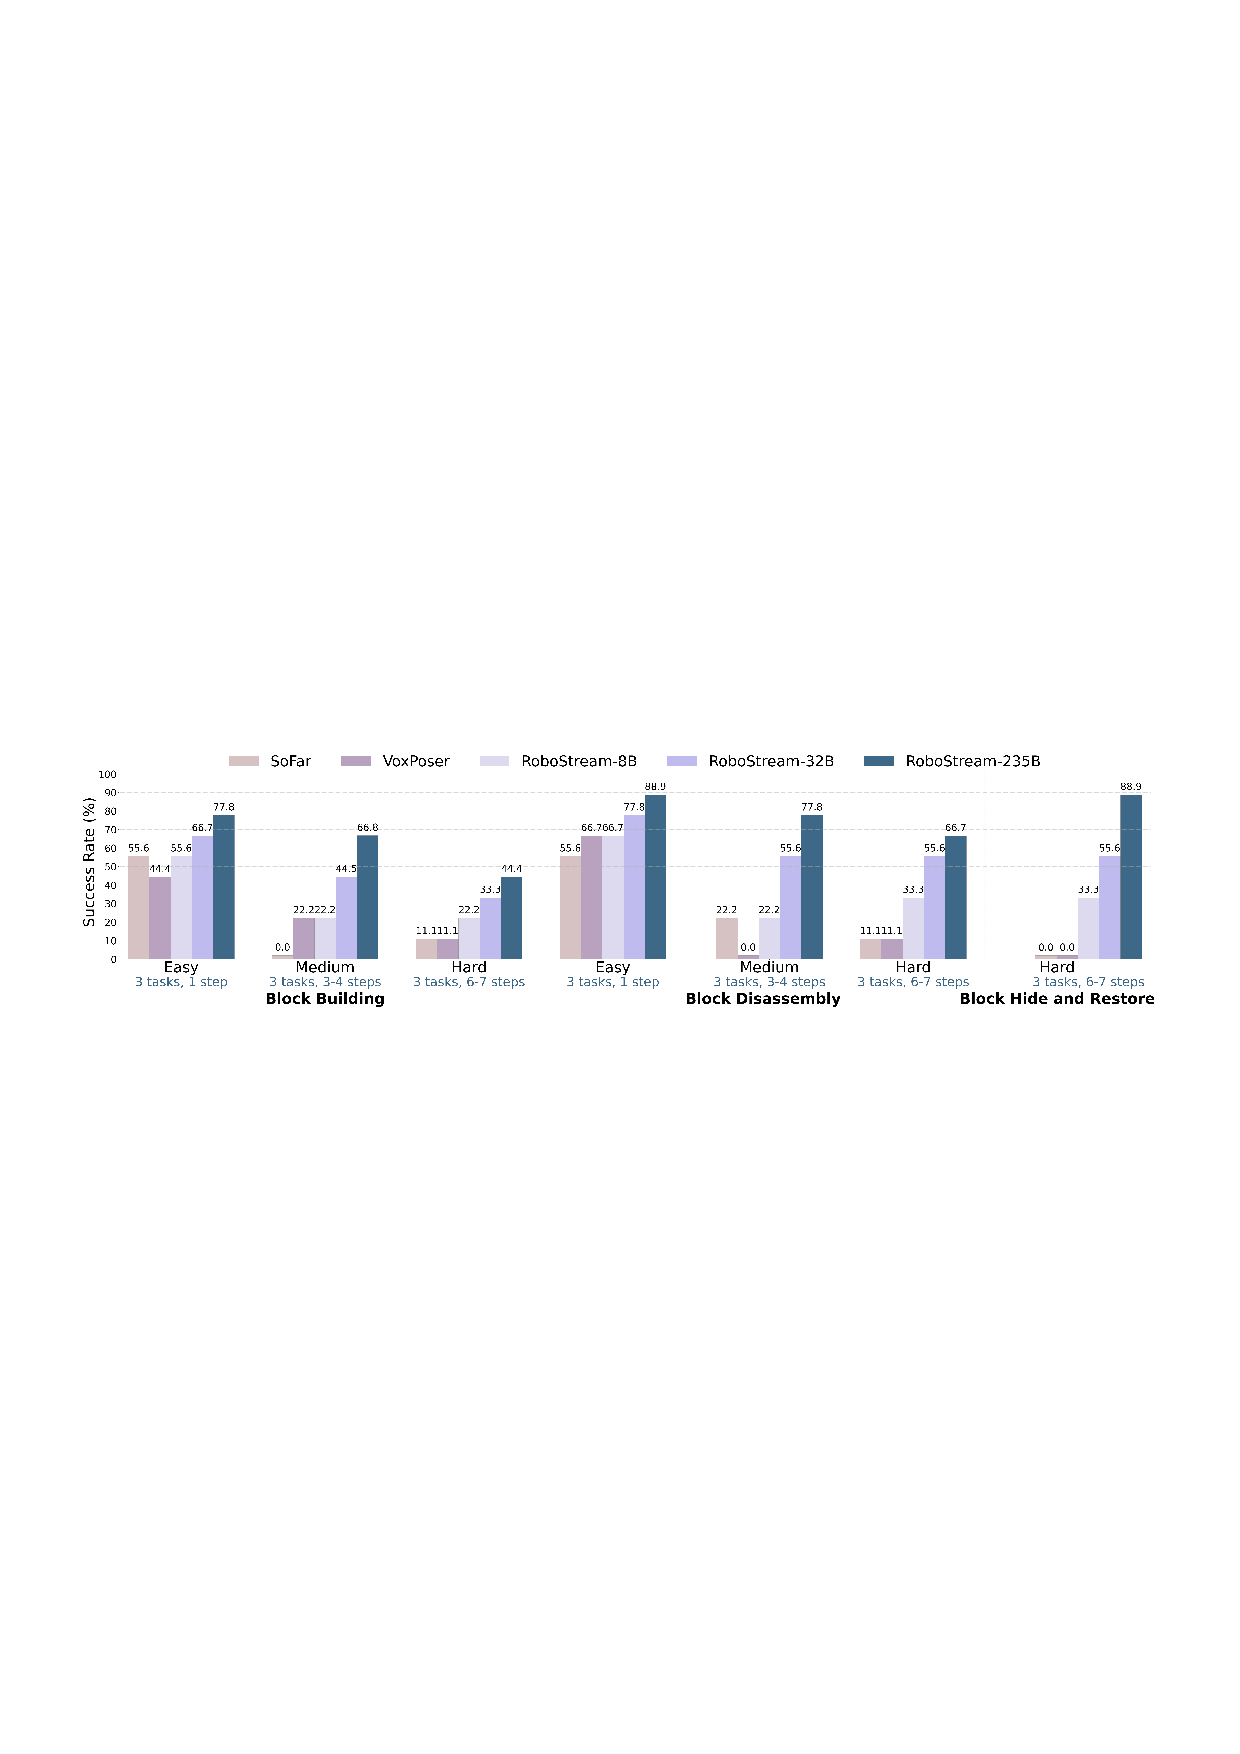
\includegraphics[width=1\textwidth]{Figures/1.pdf}
    % \caption{Performance comparison of RoboStream and baselines on real-world block building and disassembly across difficulty levels.}
    % \label{fig:real_world}
\end{figure}

\subsection{Experimental Setup}
\label{sec:setup}

We evaluate RoboStream across five benchmarks spanning physical and simulated environments, covering real-world manipulation on a Franka Research 3 arm (Sec.~\ref{sec:real_world}), long-horizon tasks on RLBench~\cite{james2020rlbench} (Sec.~\ref{sec:rlbench}), zero-shot generalization on SIMPLER~\cite{li2025evaluating} (Sec.~\ref{sec:simpler}), and 6-DoF spatial reasoning on SpatialBench~\cite{qisofar} and Open6DOR V2~\cite{ding2024open6dor} (Sec.~\ref{sec:spatial_reasoning}). short-horizon evaluation validates that the geometry grounding of STF-Tokens suppresses spatial hallucination in individual actions; long-horizon evaluation tests whether the full framework sustains causal state tracking and correct action ordering. We instantiate RoboStream with three VLM backbones, Qwen3-VL-8B, Qwen3-VL-32B, and Qwen3-VL-235B~\cite{yang2025qwen3}, hereafter referred to as RoboStream-8B, RoboStream-32B, and RoboS\-tream-235B respectively. All variants operate in a manner without environment-specific adaptation or fine-tuning across any benchmark. We compare against state-of-the-art baselines including SoFar~\cite{qisofar}, VoxPoser~\cite{huang2023voxposer}, and RT-2-X~\cite{zitkovich2023rt}, measuring execution success rate for manipulation tasks and accuracy for spatial reasoning.

To accommodate task diversity, we adopt two goal-specification strategies. For real-world experiments and RLBench long-horizon tasks, where target configurations are difficult to fully capture in text, we employ image-guided goal specification with images depicting the desired final state, such as blocks arranged in a target tower configuration. For SIMPLER short-horizon tasks, and tasks involving occlusion or state restoration, we employ text-guided natural language instructions, such as ``hide the blue cube, then restore the original state.''



\begin{figure}[t]
   
    \centering
    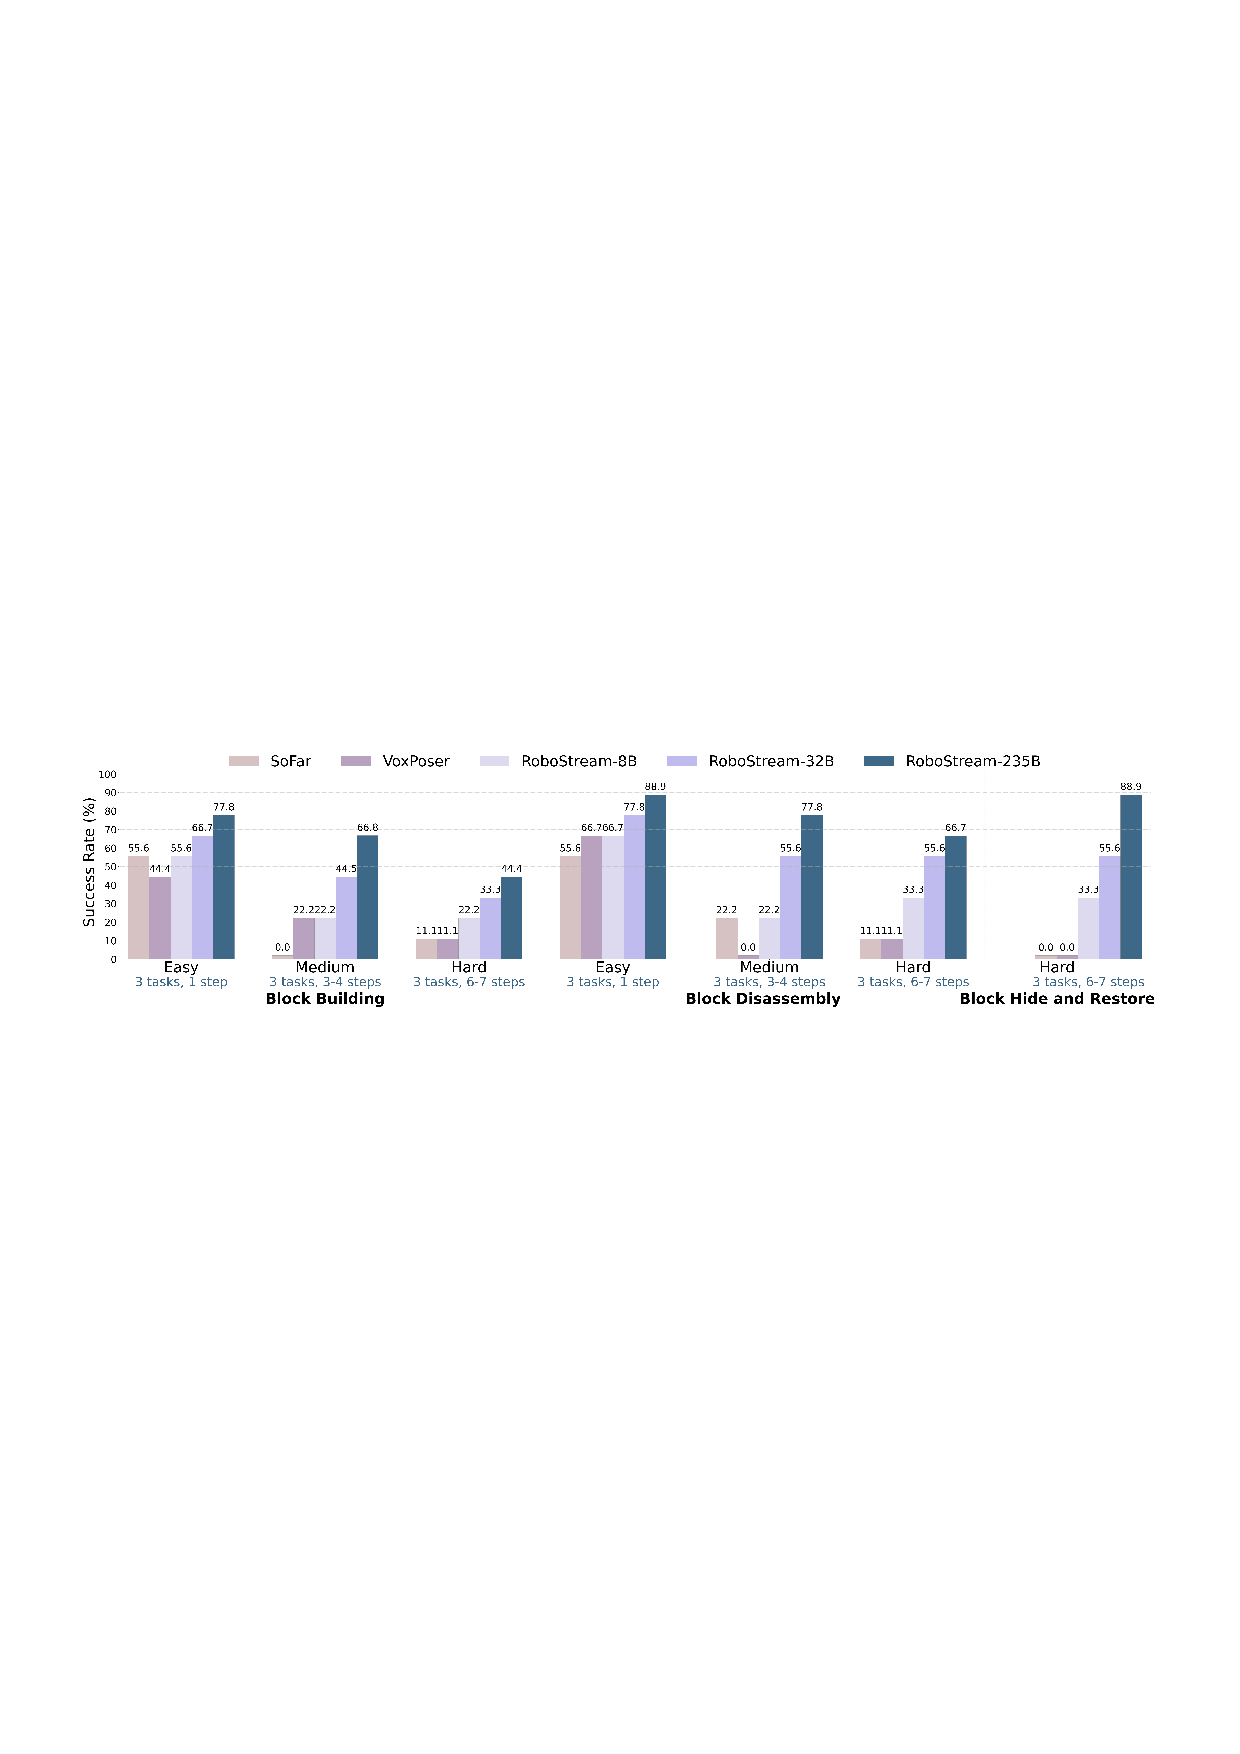
\includegraphics[width=1\textwidth]{Figures/1.pdf}
    \caption{\textbf{Performance comparison on zero-shot real-world manipulation tasks.} We design 21 diverse tasks covering block building (Task A), block disassembly (Task B), and block hide and restore (Task C).}
    \label{fig:real_world}
\end{figure}




\subsection{Real-World Robotic Manipulation}
\label{sec:real_world}
\noindent{\textbf{Tasks and Evaluations.}}~
We construct 21 real-world tasks on a Franka Research 3 (FR3) arm equipped with a parallel gripper and a front-view Intel RealSense D435i RGB-D camera, utilizing 17 colored objects, as shown in Fig.~\ref{fig:step_setting}. The tasks are categorized into three types evaluating different cognitive and physical reasoning dimensions. Task A (Block Building) assesses spatio-temporal grounding and pre-condition adherence by stacking objects Bottom-to-Top across three difficulty levels (Easy, Medium, Hard), requiring the robot to verify base stability before proceeding. Task B (Block Disassembly) evaluates sequential state tracking and support relation maintenance during Top-to-Bottom removal, requiring accurate causal memory of stacking order and support dependencies. Task C (Block Hide and Restore) stress-tests causal memory and object permanence under full occlusion, where the robot must conceal a block beneath a cup, execute distractor steps, and restore the original configuration by retrieving object identity and last known pose from causal history. Tasks A and B are specified by goal images, while Task C is guided by natural language instructions. Each task is executed three times, with details in the Appendix.




\noindent{\textbf{Results.}}~
As shown in Fig.~\ref{fig:real_world}, all RoboStream variants consistently outperform baselines across all difficulty levels, with success rates scaling proportionally with backbone capacity. On Hard-level block building and disassembly tasks, RoboStream-235B achieves success rates of 44.4\% and 66.7\%, respectively. In contrast, prior reactive systems such as SoFar~\cite{qisofar} and VoxPoser~\cite{huang2023voxposer} exhibit limited efficacy, struggling to exceed 11.1\% without persistent causal tracking and physical state evolution awareness. In Task C (Block Hide and Restore), requiring accurate tracking under total occlusion, RoboStream-235B achieves 88.9\% while even our lightweight 8B variant maintains 33.3\%, whereas SoFar and VoxPoser completely fail at 0\%. This contrast highlights that structured spatio-temporal memory is far more decisive for hidden-state tasks than scaling reactive systems. The monotonic gains across model scales confirm that STF-Tokens and CSTG provide complementary capabilities growing increasingly effective with model capacity, yielding robustness that purely reactive systems cannot replicate.

\begin{table*}[t]
    \centering
    \caption{\textbf{Quantitative success rate comparison on the SIMPLER benchmark}. We evaluate: (a) the Google Robot setup under Variant Aggregation (VA) and Visual Matching (VM) protocols, and (b) the WidowX + Bridge setup. For the WidowX tasks, we use the following abbreviations: Spoon (Put Spoon on Towel), Carrot (Put Carrot on Plate), Stack (Stack Green Block on Yellow Block), and Egg (Put Eggplant in Basket). ``Zero'' in the Data column indicates zero-shot evaluation. }
    \label{tab:simpler_env}

    % --- 左表 (Google Robot) ---
    \begin{minipage}[htbp]{0.42\linewidth}
        \centering
        \textbf{(a) Google Robot Setup}
        \vspace{2pt}

        \resizebox{\linewidth}{!}{%
        \renewcommand{\arraystretch}{1.1}
            \begin{tabular}{llcc}
                \toprule
                \textbf{Set} & \textbf{Policy} & \textbf{Pick Coke} & \textbf{Move Near} \\
                \midrule

                % --- VA 区块 ---
                \multirow{6}{*}{\textbf{VA}}
                & RT-1-X~\cite{brohan2022rt}     & 49.0 & 32.3 \\
                & RT-2-X~\cite{zitkovich2023rt}     & 82.3 & 79.2 \\
                & Octo-B~\cite{team2024octo}     & 0.6  & 3.1 \\
                & OpenVLA~\cite{kim2025openvla}    & 54.5 & 47.7 \\
                & SoFar~\cite{qisofar}      & \cellcolor{secondpurple}\underline{90.7} & \cellcolor{secondpurple}\underline{74.0} \\
                & \textbf{RoboStream-8B} & \cellcolor{firstpurple}\textbf{94.2} & \cellcolor{firstpurple}\textbf{79.8} \\
                \midrule

                % --- VM 区块 ---
                \multirow{6}{*}{\textbf{VM}}
                & RT-1-X~\cite{brohan2022rt}     & 56.7 & 31.7 \\
                & RT-2-X~\cite{zitkovich2023rt}     & 78.7 & 77.9 \\
                & Octo-B~\cite{team2024octo}     & 17.0 & 4.2 \\
                & OpenVLA~\cite{kim2025openvla}    & 16.3 & 46.2 \\
                & SoFar~\cite{qisofar}      & \cellcolor{secondpurple}\underline{92.3} & \cellcolor{secondpurple}\underline{91.7} \\
                & \textbf{RoboStream-8B} & \cellcolor{firstpurple}\textbf{95.7} & \cellcolor{firstpurple}\textbf{95.8} \\
                \bottomrule
            \end{tabular}
        }
    \end{minipage}
    \hfill
    % --- 右表 (WidowX) ---
    \begin{minipage}[htbp]{0.56\linewidth}
        \centering
        \textbf{(b) WidowX + Bridge Setup}
        \vspace{2pt}

        \renewcommand{\arraystretch}{1.11}
        \resizebox{\linewidth}{!}{%
            \begin{tabular}{llccccc}
                \toprule
                \textbf{Policy} & \textbf{Data} & \textbf{Spoon} & \textbf{Carrot} & \textbf{Stack} & \textbf{Egg} & \textbf{Avg} \\
                \midrule
                RT-1-X~\cite{brohan2022rt}      & OXE    & 0.0 & 4.2 & 0.0 & 0.0 & 1.1 \\
                Octo-B~\cite{team2024octo}      & OXE    & 12.5 & 8.3 & 0.0 & 43.1 & 16.0 \\
                Octo-S~\cite{team2024octo}      & OXE    & 47.2 & 9.7 & 4.2 & 56.9 & 30.0 \\
                OpenVLA~\cite{kim2025openvla}    & OXE    & 0.0 & 0.0 & 0.0 & 4.1 & 1.0 \\
                RoboVLM~\cite{li2026robovlm}     & OXE    & 20.8 & 25.0 & 8.3 & 0.0 & 13.5 \\
                RoboVLM~\cite{li2026robovlm}     & Bridge & 29.2 & 25.0 & 12.5 & 58.3 & 31.3 \\
                SpatialVLA~\cite{qu2025spatialvla}  & OXE    & 20.8 & 20.8 & 25.0 & 70.8 & 34.4 \\
                SpatialVLA~\cite{qu2025spatialvla}  & Bridge & 16.7 & 25.0 & 29.2 & \cellcolor{firstpurple}\textbf{100.0} & 42.7 \\
                SoFar~\cite{qisofar}       & Zero   & \cellcolor{secondpurple}\underline{58.3} & \cellcolor{secondpurple}\underline{66.7} & \cellcolor{secondpurple}\underline{70.8} & 37.5 & \cellcolor{secondpurple}\underline{58.3} \\
                \midrule
                \textbf{RoboStream-8B} & \textbf{Zero} & \cellcolor{firstpurple}\textbf{62.5} & \cellcolor{firstpurple}\textbf{71.9} & \cellcolor{firstpurple}\textbf{77.1} & \cellcolor{secondpurple}\underline{87.5} & \cellcolor{firstpurple}\textbf{74.8} \\
                \bottomrule
            \end{tabular}
        }
    \end{minipage}
\end{table*}

\subsection{Simulation Object Manipulation Evaluation on SIMPLER}
\label{sec:simpler}

We evaluate zero-shot cross-embodiment generalization on the SIMPLER benchmark~\cite{li2025evaluating} across Google Robot and WidowX + Bridge configurations, representing substantial domain shifts from training environments. These short-horizon tasks isolate STF-Token contributions by testing whether spatial grounding transfers across embodiments and viewpoints, independent of long-horizon reasoning.

\noindent{\textbf{Google Robot Configuration.}}~
As shown in Tab.~\ref{tab:simpler_env}, RoboStream-8B achieves superior success rates on both ``Pick Coke Can'' and the spatially demanding ``Move Near'' tasks under VM evaluation, surpassing the prior state-of-the-art SoFar~\cite{qisofar}. Notably, RoboStream-8B also outperforms OXE-finetuned RT-2-X~\cite{zitkovich2023rt} by a substantial margin despite operating fully zero-shot. Under the more challenging VA evaluation, RoboStream-8B maintains competitive performance, again exceeding SoFar. Consistent gains across both protocols and tasks with varying geometry confirm stable spatial grounding independent of embodiment.

\noindent{\textbf{WidowX + Bridge Configuration.}}~
RoboStream achieves a higher average success rate across all subtasks compared to zero-shot SoFar and Bridge-finetuned SpatialVLA~\cite{qu2025spatialvla} without requiring any fine-tuning or domain adaptation. Notably, this advantage holds despite SpatialVLA being explicitly trained on in-domain Bridge data, highlighting the superior transferability of our geometry-grounded representation. These results confirm that spatio-temporal reasoning grounded in explicit geometric primitives transfers robustly across embodiments and extends naturally from short tasks to subsequent long-horizon benchmarks.





\subsection{Simulation Long-Horizon Task Evaluation on RLBench}
\label{sec:rlbench}


\begin{table}[t]
\centering
\caption{\textbf{Simulation evaluation of long-horizon manipulation on RLBench.} All RoboStream variants are evaluated in a zero-shot manner without in-domain fine-tuning. }
\label{tab:full_vertical_compact}
\resizebox{\textwidth}{!}{
\begin{tabular}{l ccccc}
\toprule
\textbf{Tasks} & 
\textbf{SoFar}~\cite{qisofar} & 
\textbf{VoxPoser}~\cite{huang2023voxposer} & 
\textbf{RoboStream-8B} & 
\textbf{RoboStream-32B} & 
\textbf{RoboStream-235B} \\
\midrule
Bridge Between Towers            & 52.0 & 8.0 & \cellcolor{secondpurple}\underline{76.0} & \cellcolor{firstpurple}\textbf{88.0} & \cellcolor{firstpurple}\textbf{88.0} \\
Cover Top Block with Box         & 4.0 & 4.0 & 40.0 & \cellcolor{secondpurple}\underline{84.0} & \cellcolor{firstpurple}\textbf{92.0} \\
Cover Bottom Block with Box      & 0.0 & 0.0 & 16.0 & \cellcolor{secondpurple}\underline{68.0} & \cellcolor{firstpurple}\textbf{96.0} \\
Place Blocks in Two Containers   & \cellcolor{firstpurple}\textbf{100.0} & \cellcolor{secondpurple}\underline{96.0} & \cellcolor{firstpurple}\textbf{100.0} & \cellcolor{firstpurple}\textbf{100.0} & \cellcolor{firstpurple}\textbf{100.0} \\
Place Blocks in Two Cont. (Hard) & 4.0 & 4.0 & 24.0 & \cellcolor{secondpurple}\underline{76.0} & \cellcolor{firstpurple}\textbf{88.0} \\
Stack Five Colors                & 4.0 & 4.0 & 60.0 & \cellcolor{secondpurple}\underline{72.0} & \cellcolor{firstpurple}\textbf{80.0} \\
Stack Three Colors               & \cellcolor{secondpurple}\underline{60.0} & \cellcolor{firstpurple}\textbf{96.0} & \cellcolor{firstpurple}\textbf{96.0} & \cellcolor{firstpurple}\textbf{96.0} & \cellcolor{firstpurple}\textbf{96.0} \\
Unstack then Stack Four Colors   & 0.0 & 0.0 & 52.0 & \cellcolor{secondpurple}\underline{76.0} & \cellcolor{firstpurple}\textbf{84.0} \\
\midrule
\textbf{Average}                     & 28.0 & 26.5 & 58.0 & \cellcolor{secondpurple}\underline{82.5} & \cellcolor{firstpurple}\textbf{90.5} \\
\bottomrule
\end{tabular}
}
\end{table}

\noindent{\textbf{Tasks and Evaluations.}}~
To assess long-horizon manipulation capabilities, we introduce 8 complex tasks within RLBench~\cite{james2020rlbench} (Tab.~\ref{tab:full_vertical_compact}), constructed by extending and reconfiguring native assets. Each method is evaluated over 25 episodes per task using different random seeds. Following Sec.~\ref{sec:setup}, tasks are categorized by guidance modality. Five goal-image-guided tasks require visually complex target configurations, including Bridge Between Towers, Place Blocks in Two Containers, Place Blocks in Two Cont. (Hard), and Stack Three/Five Colors. Three text-guided tasks stress-test action ordering, restoration, and object permanence under occlusion, including Cover Top/Bottom Block with Box and Unstack then Stack Four Colors. Detailed setups are provided in the Appendix.

\noindent{\textbf{Results.}}~
As shown in Tab.~\ref{tab:full_vertical_compact}, RoboStream consistently outperforms both SoFar~\cite{qisofar} and VoxPoser~\cite{huang2023voxposer} across these long-horizon scenarios. Notably, our framework demonstrates a strong scaling effect, with performance increasing alongside model capacity to reach a 90.5\% average success rate on RoboStream-235B without additional training, as larger capacity provides the reasoning depth necessary to maintain logical consistency over extended action sequences. However, scaling the VLM alone is not a panacea for long-horizon stability. Even our smallest variant, RoboStream-8B, substantially exceeds much larger baselines, demonstrating that spatio-temporal reasoning and structured memory are more critical for physical consistency than simply increasing parameter scale.










\begin{table}[t]
    \centering
    % --- 左侧表格 ---
    \begin{minipage}[t]{0.56\textwidth} 
        \centering
        \vspace{0em}
        \setlength{\tabcolsep}{2.5pt} 
        \caption{\textbf{Spatial reasoning evaluation on 6-DoF SpatialBench~\cite{qisofar}.} Results are categorized by spatial VQA task types, covering absolute ($abs.$) and relative ($rel.$) reasoning for both position and orientation.}
        \label{tab:spatial_reasoning_final}
        \scriptsize
        \begin{tabular}{@{}lccccc@{}}
        \toprule
        \multirow{2}{*}{Method} & \multicolumn{2}{c}{Position} & \multicolumn{2}{c}{Orientation} & \multirow{2}{*}{Total} \\
        \cmidrule(lr){2-3} \cmidrule(lr){4-5}
        & rel. & abs. & rel. & abs. & \\
        \midrule
        GPT-4o~\cite{hurst2024gpt}      & 49.4 & 28.4 & 44.2 & 25.8 & 36.2 \\
        SpaceMantis~\cite{chen2024spatialvlm} & 33.6 & 29.2 & 27.2 & 25.0 & 28.9 \\
        RoboPoint~\cite{yuan2025robopoint}   & 43.8 & 30.8 & 33.8 & 25.8 & 33.5 \\
        SoFar~\cite{qisofar} & 59.6 & 33.8 & \cellcolor{firstpurple}\textbf{54.6} & 31.3 & 43.9 \\
        SoFar-8B~\cite{qisofar} & 41.5 & 24.3 & 27.1 & 31.3 & 30.5 \\
        SoFar-32B~\cite{qisofar} & \cellcolor{secondpurple}\underline{60.4} & \cellcolor{secondpurple}\underline{41.9} & 45.8 & 33.3 & \cellcolor{secondpurple}\underline{45.3} \\
        \textbf{RoboStream-8B} & 47.2 & 31.1 & 35.4 & \cellcolor{secondpurple}\underline{35.4} & 36.8 \\
        \textbf{RoboStream-32B} & \cellcolor{firstpurple}\textbf{66.0} & \cellcolor{firstpurple}\textbf{44.6} & \cellcolor{secondpurple}\underline{48.0} & \cellcolor{firstpurple}\textbf{37.5} & \cellcolor{firstpurple}\textbf{48.9} \\
        \bottomrule
        \end{tabular}
    \end{minipage}
    \hfill 
    % --- 右侧表格 ---
    \begin{minipage}[t]{0.42\textwidth} % 保持宽度 0.42
        \centering
        \setlength{\tabcolsep}{2pt} % 保持 2pt
        \renewcommand{\arraystretch}{1.18} % 
        \caption{\textbf{6-DoF object rea\-r\-r\-a\-n\-g\-e\-m\-e\-n\-t evaluation on O\-p\-e\-n\-6\-D\-O\-R~\cite{ding2024open6dor}.} Results are categorized by position ($Pos.$), rotation ($Rot.$), and integrated 6-DoF success rates. }
        \label{tab:open6dor_updated}
        \scriptsize 
        \begin{tabular}{@{}lccc@{}}
        \toprule
        Method & Pos.  & Rot.  & 6-DoF  \\
        \midrule
        Dream2Real~\cite{kapelyukh2024dream2real}         & 15.9 & 31.3 & 13.5 \\
        VoxPoser~\cite{huang2023voxposer}            & 32.6 & -    & -    \\
        Open6DOR-GPT~\cite{ding2024open6dor}       & 74.9 & 41.1 & 35.6 \\
        SoFar~\cite{qisofar}          & 93.0 & \cellcolor{secondpurple}\underline{57.0} & \cellcolor{secondpurple}\underline{48.7} \\
        SoFar-8B~\cite{qisofar}               & 92.4 & 42.9 & 45.1 \\
        SoFar-32B~\cite{qisofar}              & \cellcolor{secondpurple}\underline{93.1} & 54.6 & 48.4 \\
        \textbf{RoboStream-8B}          & \cellcolor{secondpurple}\underline{93.1} & 47.6 & 47.3 \\
        \textbf{RoboStream-32B}& \cellcolor{firstpurple}\textbf{93.8} & \cellcolor{firstpurple}\textbf{58.8} & \cellcolor{firstpurple}\textbf{52.2} \\
        \bottomrule
        \end{tabular}
    \end{minipage}
\end{table}



\subsection{6-DoF Spatial Reasoning Evaluation}
\label{sec:spatial_reasoning}
To evaluate how STF-Tokens bridge high-level visual features with precise instance-level 3D grounding, we extend our evaluation to rotation and full 6-DoF pose estimation. Following SoFar~\cite{qisofar}, we incorporate PointSO for 6-DoF prediction and evaluate on Open6DOR V2~\cite{ding2024open6dor} and 6-DoF SpatialBench~\cite{qisofar}. Since SoFar serves as our primary baseline, we include variants using Qwen3-VL-8B and Qwen3-VL-32B backbones for fair cross-scale comparison with RoboStream.



\noindent{\textbf{Spatial Reasoning on 6-DoF SpatialBench.}}~
As shown in Tab.~\ref{tab:spatial_reasoning_final}, RoboStream-32B achieves superior overall performance, outperforming both SoFar and GPT-4o~\cite{hurst2024gpt}. The most pronounced gains appear on absolute and relative position tasks, where pure image-text alignment is most susceptible to spatial ambiguity. These results confirm that the core advantage of STF-Tokens lies not in coordinate injection alone, but in serving as a geometric anchor providing deterministic spatial reference when visual features and language descriptions conflict.



\noindent{\textbf{6-DoF Object Rearrangement on Open6DOR V2.}}~
As shown in Tab.~\ref{tab:open6dor_updated}, RoboStream-32B consistently outperforms SoFar across position, rotation, and integrated 6-DoF metrics. Unlike baselines treating spatial coordinates as text annotations, STF-Tokens distill per-object visual evidence into structured instance representations encoding centroid, Gaussian shape, and orientation. This shift from pixel-level to object-level reasoning underlies consistent gains across all tracks, most notably on 6-DoF where tight placement constraints demand precise geometric grounding and spatial alignment.

\begin{table*}[t]
\centering
\caption{\textbf{Ablation study on RoboStream-235B.} Success rates (\%) across 8 long-horizon tasks, isolating contributions of CSTG and STF-Tokens.}
\label{tab:ablation_235b_horizontal}
\resizebox{\textwidth}{!}{%
\renewcommand{\arraystretch}{1.2} % 稍微增加行高，让色块更美观
\begin{tabular}{cc | ccccccccc}
\toprule
\thead{\textit{STF-} \\ \textit{Tokens}} & \thead{\textit{CSTG}} &
 \thead{Bridge Between\\Towers} & 
 \thead{Cover Top\\Block} & 
 \thead{Cover Bottom\\Block} & 
 \thead{Place in\\Containers} & 
 \thead{Place in\\Containers (Hard)} & 
 \thead{Stack Five\\Colors} & 
 \thead{Stack Three\\Colors} & 
 \thead{Unstack then\\Stack} & 
 \textbf{Average} \\
\midrule
% w/o Both (Baseline)
\xmark & \xmark & 0.0 & 0.0 & 0.0 & 84.0 & 12.0 & 0.0 & 0.0 & 0.0 & 12.0 \\
% w/o CSTG
\cmark & \xmark & 0.0 & 0.0 & 0.0 & \cellcolor{secondpurple}\underline{92.0} & 24.0 & 0.0 & 0.0 & 0.0 & 14.5 \\
% w/o STF-Tokens
\xmark & \cmark & \cellcolor{secondpurple}\underline{72.0} & \cellcolor{secondpurple}\underline{84.0} & \cellcolor{secondpurple}\underline{88.0} & \cellcolor{firstpurple}\textbf{100.0} & \cellcolor{secondpurple}\underline{72.0} & \cellcolor{secondpurple}\underline{60.0} & \cellcolor{firstpurple}\textbf{96.0} & \cellcolor{secondpurple}\underline{64.0} & \cellcolor{secondpurple}\underline{79.5} \\
% Full Model
\cmark & \cmark & \cellcolor{firstpurple}\textbf{88.0} & \cellcolor{firstpurple}\textbf{92.0} & \cellcolor{firstpurple}\textbf{96.0} & \cellcolor{firstpurple}\textbf{100.0} & \cellcolor{firstpurple}\textbf{88.0} & \cellcolor{firstpurple}\textbf{80.0} & \cellcolor{firstpurple}\textbf{96.0} & \cellcolor{firstpurple}\textbf{84.0} & \cellcolor{firstpurple}\textbf{90.5} \\
\bottomrule
\end{tabular}%
}
\end{table*}



\subsection{Ablation Study}
\label{sec:ablation_study}

We ablate RoboStream-235B across all 8 long-horizon RLBench~\cite{james2020rlbench} tasks to isolate the contribution of each architectural component (Tab.~\ref{tab:ablation_235b_horizontal}). Removing the CSTG module (\textit{w/o CSTG}) causes the average success rate to collapse from 90.5\% to 14.5\%, confirming that persistent state tracking is the foundational driver for long-horizon tasks. However, while CSTG provides logical structure, STF-Tokens provide physical precision. Removing STF-Tokens (\textit{w/o STF-Tokens}) results in an 11.0\% absolute drop (from 90.5\% to 79.5\%), demonstrating that without explicit 3D geometric grounding, even a CSTG-equipped agent struggles with compounding spatial inaccuracies during contact-rich execution. The mutual dependence of both components becomes evident when removing them simultaneously (\textit{w/o Both}), which yields only 12.0\% success rate. Notably, comparing this to the \textit{w/o CSTG} variant (14.5\%) shows that STF-Tokens still provide marginal improvement in short-horizon spatial accuracy even when long-horizon logic fails. Their full potential, however, is unlocked only when coupled with the CSTG, where CSTG ensures correct action sequencing and STF-Tokens ensure each step is executed with deterministic spatial precision.

% %3.5 12:29 wujie修改
% We ablate RoboStream-235B across eight long-horizon RLBench tasks to isolate the contribution of each architectural component (Tab.~\ref{tab:ablation_235b_horizontal}). Removing the causal memory log (\textit{w/o Memory}) leads to a catastrophic performance collapse, confirming that persistent state tracking is the foundational driver for long-horizon tasks. While memory provides logical structure, STF-Tokens offer essential physical precision. Eliminating STF-Tokens (\textit{w/o STF-Tokens}) results in a significant performance drop, demonstrating that without explicit 3D geometric grounding, even a memory-equipped agent struggles with compounding spatial inaccuracies during contact-rich execution. The mutual dependence of both components becomes evident in the \textit{w/o Both} variant, which fails to complete nearly all tasks. Notably, comparing this to the \textit{w/o Memory} baseline suggests that STF-Tokens still provide marginal improvements in local spatial accuracy even when long-horizon logic fails. Their full potential, however, is unlocked only when coupled with the causal memory log: memory ensures correct action sequencing, while STF-Tokens guarantee that each step is executed with deterministic spatial precision.
% \vspace{-1em}
% \section{Conclusion}
\label{sec:conclusion}
RoboStream addresses two representation deficits that cause VLM-based planners to fail on long-horizon manipulation. The first is Ungrounded Spatial Perception, where geometry from raw pixels allows small inaccuracies to compound into spatial hallucinations. The second is Untracked Causal History, where absent action-state records leave planners unaware of displaced or occluded objects. STF-Tokens resolve the first via Spatio-Temporal Grounding by distilling per-object appearance and 3D geometry into identity-persistent primitives. The CSTG resolves the second via Causal Memory Tracking by maintaining persistent records of state transitions, enabling inference of hidden object states. Across five benchmarks including RLBench, SIMPLER, SpatialBench, Open6DOR V2, and real-world Franka experiments, RoboStream consistently outperforms existing methods, establishing that weaving spatio-temporal reasoning with persistent memory is more decisive for long-horizon stability than model scale alone.
% \section{Limitation}
\label{sec:limitation}
As a decoupled planning-execution framework, RoboStream shares a limitation inherent to the broader VLM-for-robotics paradigm. Imperfections in any sub-module, including unstable grasping or perceptual uncertainty, can propagate into execution failures even when high-level planning is correct. This reflects a fundamental tension between semantic generalization of VLM-based planners and physical precision demanded by low-level control, a challenge broadly applicable to decoupled systems beyond RoboStream. Future work includes exploring hybrid approaches that bridge VLM planner generalization with end-to-end execution fluency, either by adopting a Vision-Language-Action (VLA) model as the downstream controller for smoother and more compliant motion, or by developing a fully end-to-end VLA that internalizes spatio-temporal reasoning and causal memory within the action generation loop. Extending RoboStream to contact-rich, dexterous, and open-world manipulation also constitutes a promising direction.

% \clearpage
% \bibliographystyle{splncs04}
% \bibliography{main}


\clearpage
\appendix


\section{Appendix}
\subsection{Robot Setups}
\subsubsection{Simulation Robot Setups}
We run all simulation experiments in two benchmarks: RLBench~\cite{james2020rlbench} and SIMPLER~\cite{li2025evaluating}.  

\textbf{(a) RLBench setup.} We use the standard RLBench environment equipped with a Franka Emika Panda (7-DoF) arm and a Panda Gripper, utilizing a planning-based control stack. Our approach relies primarily on the front RGB-D camera as the main visual observation for planning. We report results on 15 single-step tasks and 8 long-horizon multi-step tasks.

\textbf{(b) SIMPLER setup.} We evaluate two embodiments in SIMPLER: Google Robot and WidowX + Bridge. For visual observations, we utilize the overhead camera for the Google Robot and the 3rd-view camera for WidowX. Crucially, we apply our training-free planning pipeline directly across both configurations without any environment-specific fine-tuning.

\subsubsection{Real World Robot Setups}
% 在真机实验中，我们统一使用了Franka Research 3 arm，搭配一对夹爪，使用front view的Real Sense D435i型号RGB-D摄像头获取视觉信息和深度信息进行点云重建。如图是workspace和机械臂的示意图。（放一张抠出来的机械臂图片，一张侧面拍的工作环境示意图

In our real-world experiments, we uniformly utilized a Franka Research 3 (FR3) robotic arm equipped with a parallel gripper. A front-view Intel RealSense D435i RGB-D camera was deployed to capture both visual and depth information for point cloud reconstruction. The detailed workspace and robot configurations are illustrated in Fig.~\ref{fig:appendix_robot_setup}.

\begin{figure}[htbp]
    \centering
    \newlength{\robotheight}\settoheight{\robotheight}{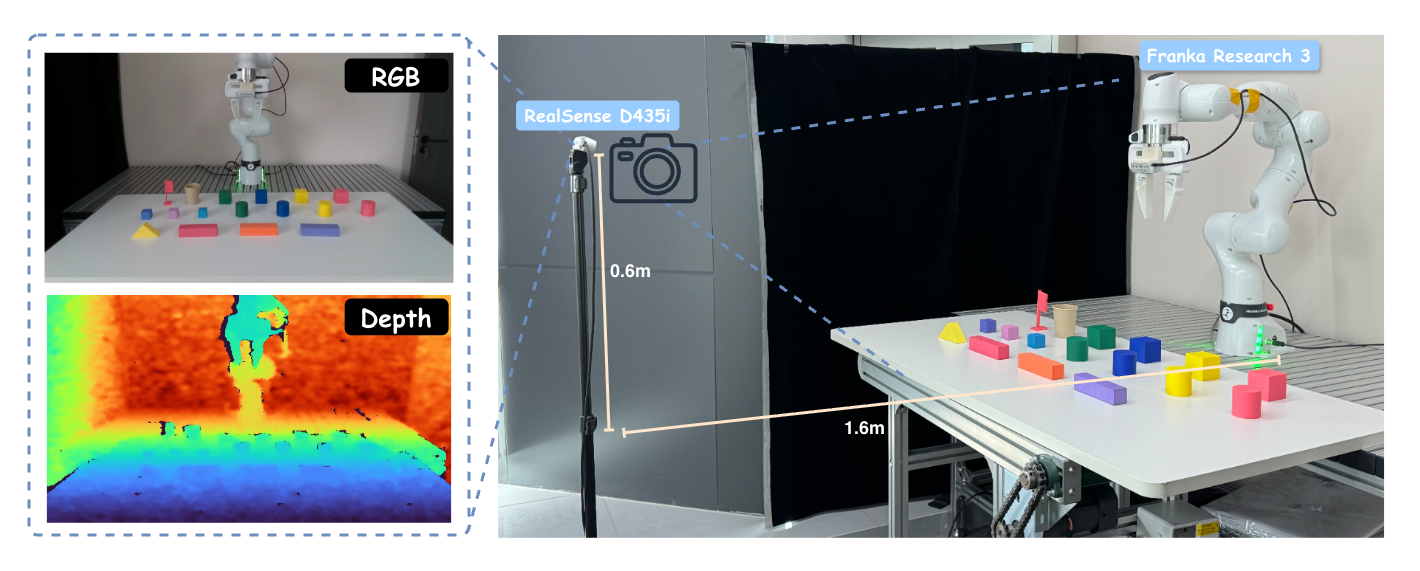
\includegraphics[width=0.72\textwidth]{Figures/appendix_robotenv.png}}%
    \begin{subfigure}[b]{0.25\textwidth}
        \centering
        \includegraphics[height=\robotheight]{Figures/appendix_franka.pdf}
        \caption{Franka Research 3.}
        \label{fig:appendix_franka}
    \end{subfigure}
    \hfill
    \begin{subfigure}[b]{0.72\textwidth}
        \centering
        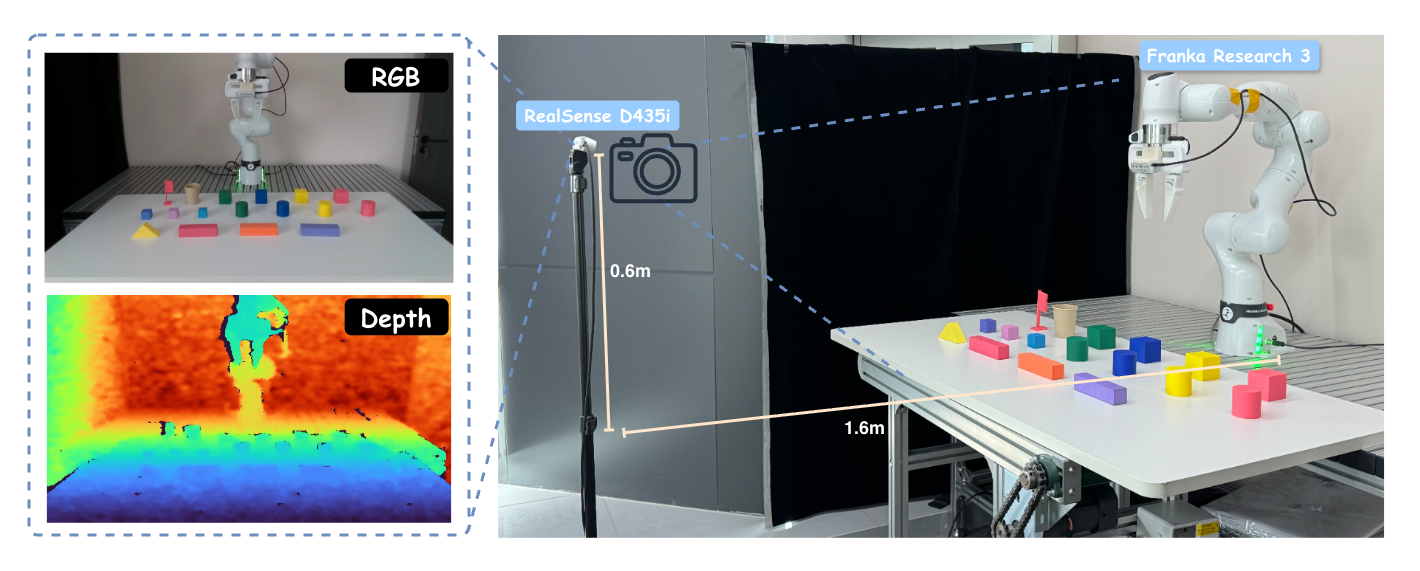
\includegraphics[width=\textwidth]{Figures/appendix_robotenv.png}
        \caption{Workspace setup with RGB and depth views.}
        \label{fig:appendix_robotenv}
    \end{subfigure}
    \caption{\textbf{Real-world experimental setup.} (a) The Franka Research 3 robot arm used in our experiments. (b) The physical workspace equipped with the robot arm and an Intel RealSense D435i camera; the insets show the corresponding RGB view and depth map.}
    \label{fig:appendix_robot_setup}
\end{figure}
\subsection{Experimental Assets and Task Design}
\noindent\textbf{Real-World Experimental Assets.} 
As shown in Fig.~\ref{fig:appendix_assets}, our real-world experiments utilize a diverse set of manipulation objects designed to evaluate precise spatial reasoning and sequential stacking. These assets primarily consist of: 
(i) \textit{Geometric primitives} including rectangular blocks, cubes, and cylinders in various sizes and distinct colors (pink, blue, green, yellow, purple, and orange); 
(ii) \textit{A triangular prism} (yellow triangle in Fig.~\ref{fig:appendix_assets}) used for assessing high-precision alignment and challenging placement tasks; and 
(iii) \textit{Functional objects} (e.g., a pink flag and a brown cup) to create dynamic occlusion and nesting scenarios. 
In total, these 17 unique pieces allow for a vast combinatorial space of long-horizon tasks, such as multi-layer block building and disassembling, providing a rigorous testbed for the model's object permanence and spatial consistency.

\begin{figure}[htbp]
    \centering
    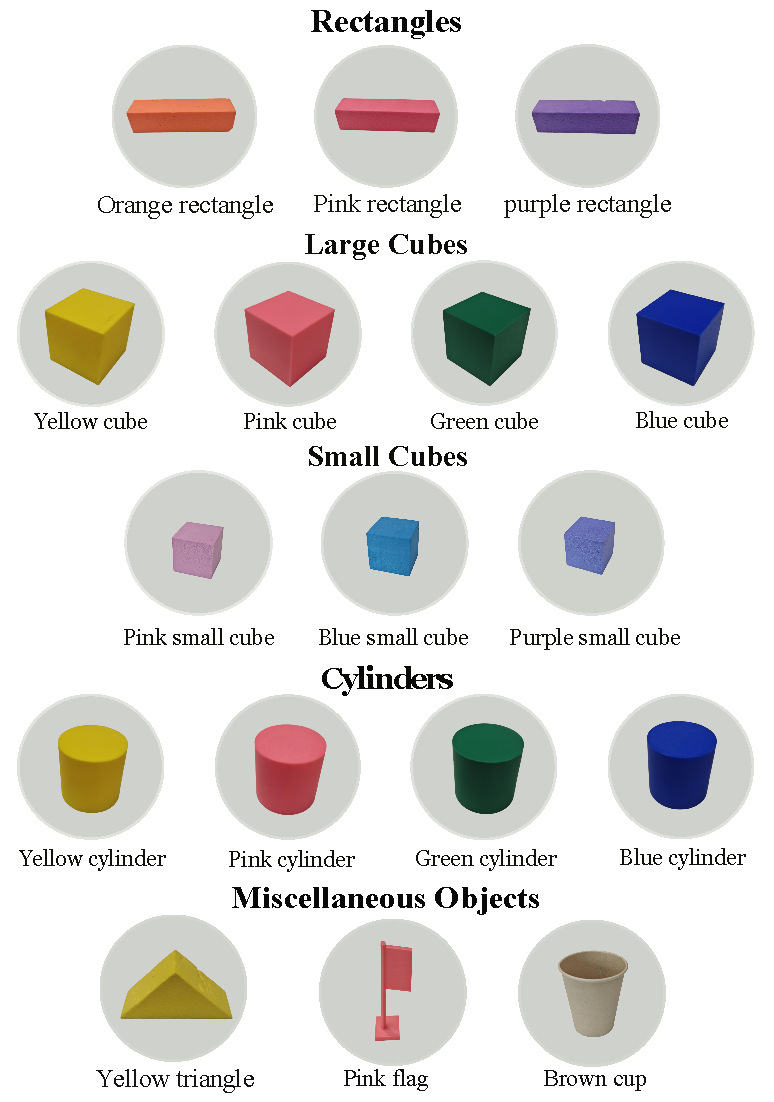
\includegraphics[width=0.6\textwidth]{Figures/appendix_assets.pdf} 
    \caption{\textbf{Assets for real-world experiments.} A collection of 17 manipulation objects including geometric primitives, a triangular prism, and functional objects used across all task difficulty levels.}
    \label{fig:appendix_assets}
\end{figure}

\subsubsection{Design of Real World Tasks}

Building on the experimental setup described in Sec.~\ref{sec:real_world}, we detail the task design across three difficulty levels. All tasks use the same Franka FR3 platform and RGB-D sensing described above.

\begin{itemize}
    \item \textbf{Easy \& Medium (Fig.~\ref{fig:appendix_step1}, \ref{fig:appendix_step2}):} Easy tasks involve 2--3 objects with single-step pick-and-place actions. Medium tasks extend to 4 objects and 3--4 sequential steps, requiring strict execution order. Both levels evaluate basic visual-language grounding and spatial precision.
    
    \item \textbf{Hard Block Building \& Disassembly (Fig.~\ref{fig:appendix_step3}):} These tasks involve up to 7 objects and 6--7 sequential actions. Building follows a Bottom-to-Top layer order for structural stability, while disassembly requires Top-to-Bottom single-anchor chaining to prevent collapse. These configurations test the model's understanding of physical support relationships over extended horizons.
    
    \item \textbf{Memorize \& Restore under Occlusion (Fig.~\ref{fig:appendix_step4}):} The robot hides an object (e.g., covering a cube with a cup), executes intermediate distractor actions, and must later recall the hidden object's location to restore the original scene. This directly evaluates causal memory retention and object permanence under occlusion---capabilities that purely reactive visual systems lack.
\end{itemize}

% --- Figures Below ---

\begin{figure}[htbp]
    \centering
    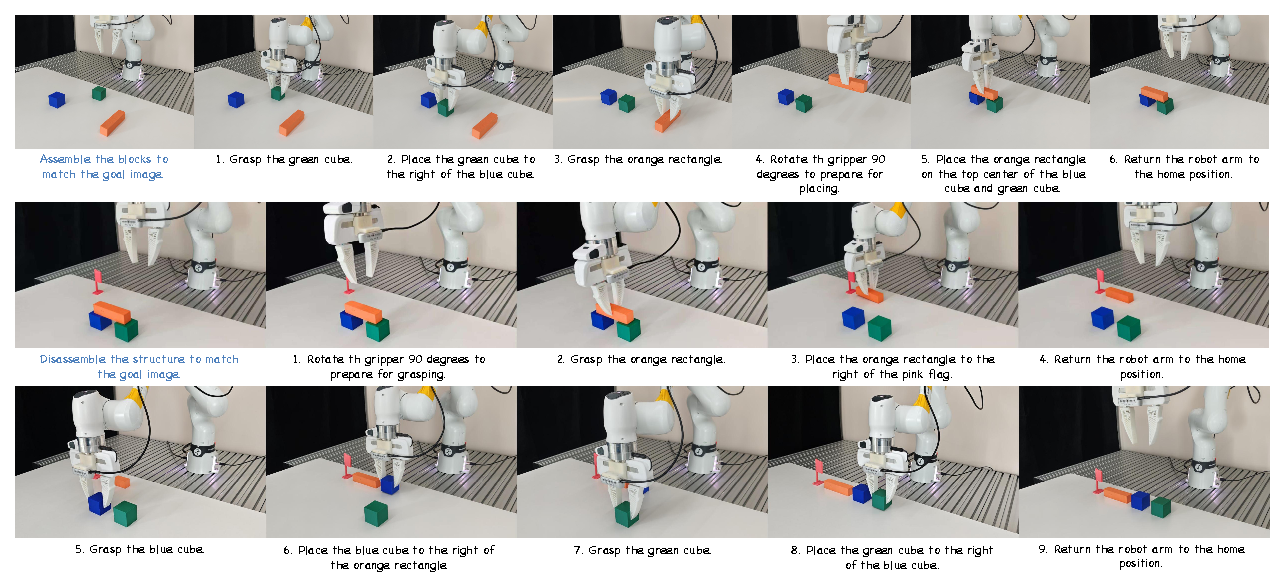
\includegraphics[width=1\textwidth]{Figures/appendix_realworld1.pdf} 
    \caption{\textbf{Multi-step block manipulation (Easy).} Execution of basic assembly and disassembly involving 2--3 objects, demonstrating fundamental spatial grounding and pick-and-place precision.}
    \label{fig:appendix_step1}
\end{figure}

\begin{figure}[htbp]
    \centering
    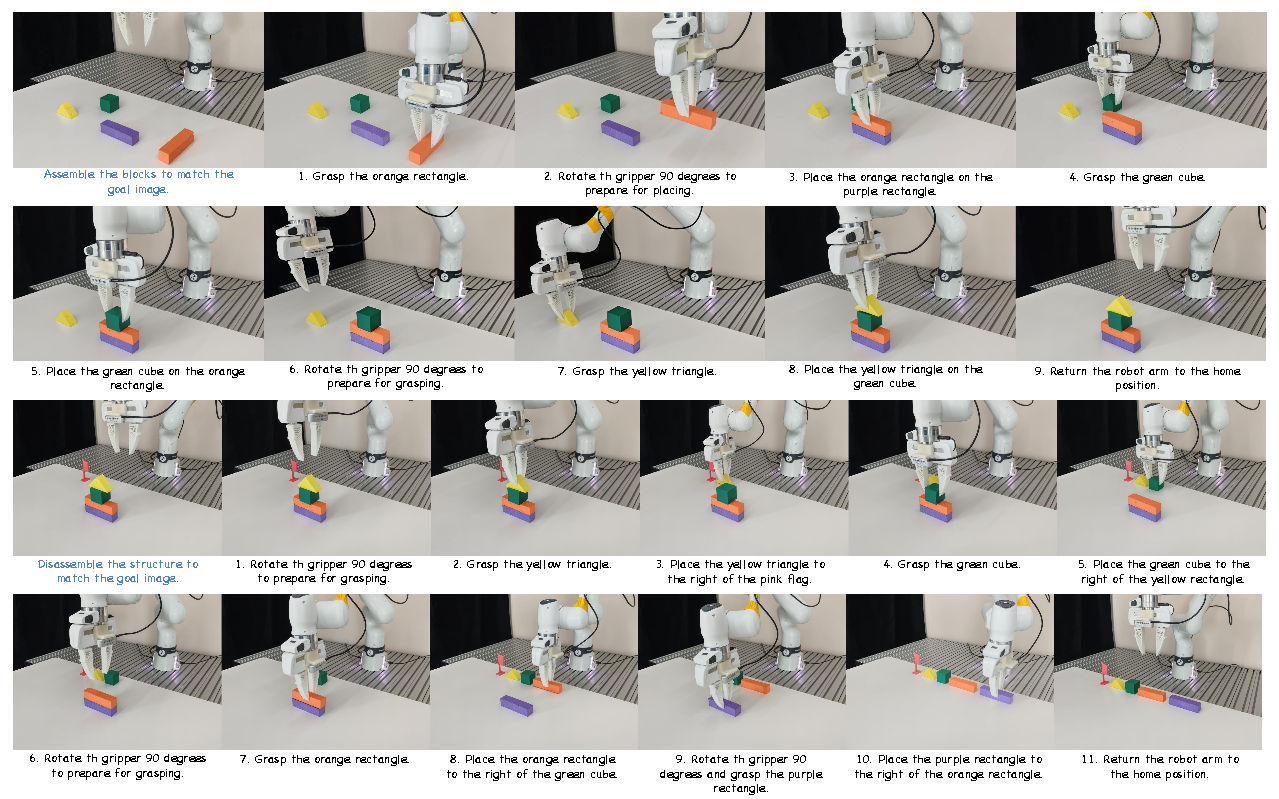
\includegraphics[width=1\textwidth]{Figures/appendix_realworld2.pdf} 
    \caption{\textbf{Multi-step block manipulation (Medium).} Intermediate execution requiring a strict sequence of 3--4 steps to manipulate 4 objects, verifying short-horizon sequential planning.}
    \label{fig:appendix_step2}
\end{figure}

\begin{figure}[htbp]
    \centering
    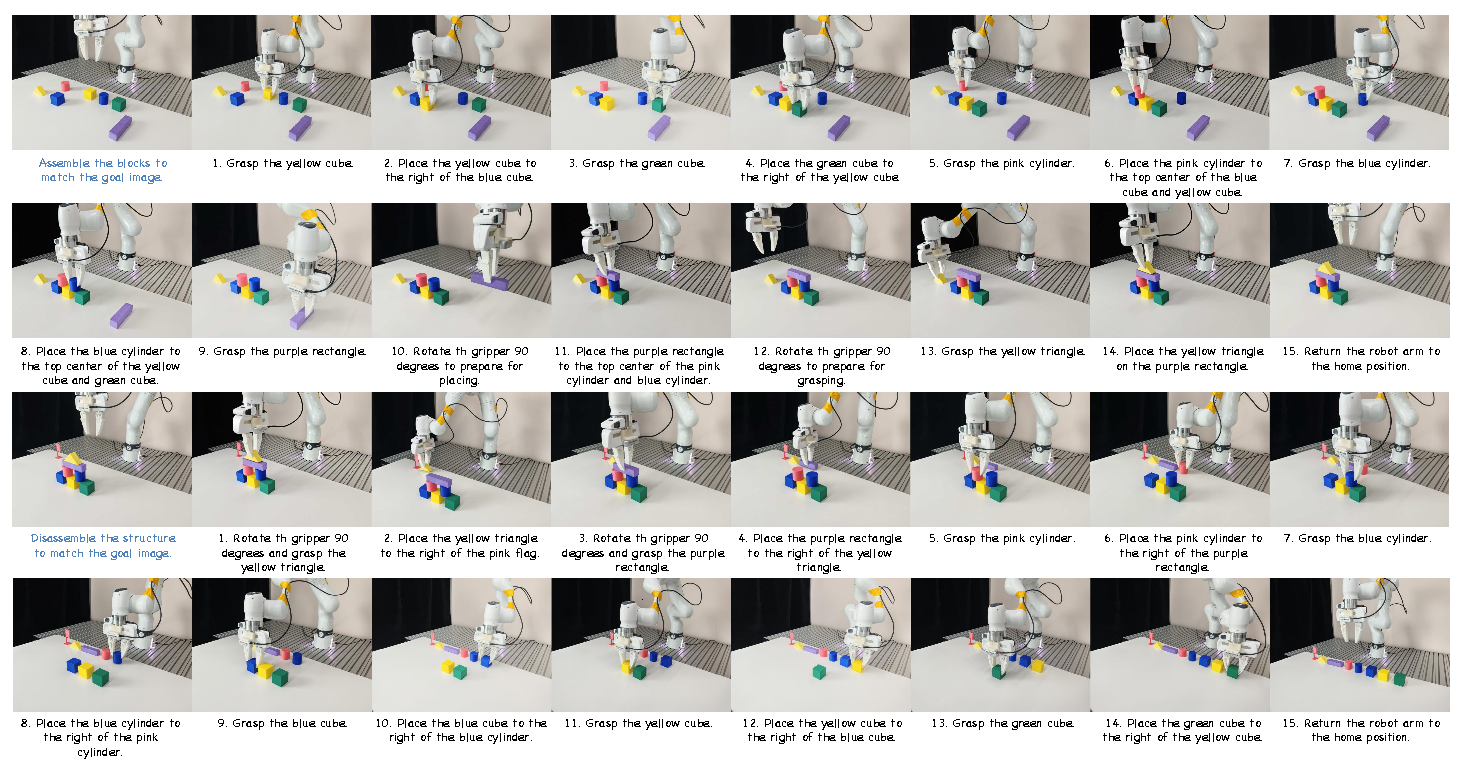
\includegraphics[width=1\textwidth]{Figures/appendix_realworld3.pdf} 
    \caption{\textbf{Multi-step block manipulation (Hard).} Extreme long-horizon execution involving 7 objects and 6--7 steps. The sequence highlights the model's ability to maintain physical stability during complex ``Bottom-to-Top'' building and ``Top-to-Bottom'' disassembly without collapsing the structure.}
    \label{fig:appendix_step3}
\end{figure}

\begin{figure}[htbp]
    \centering
    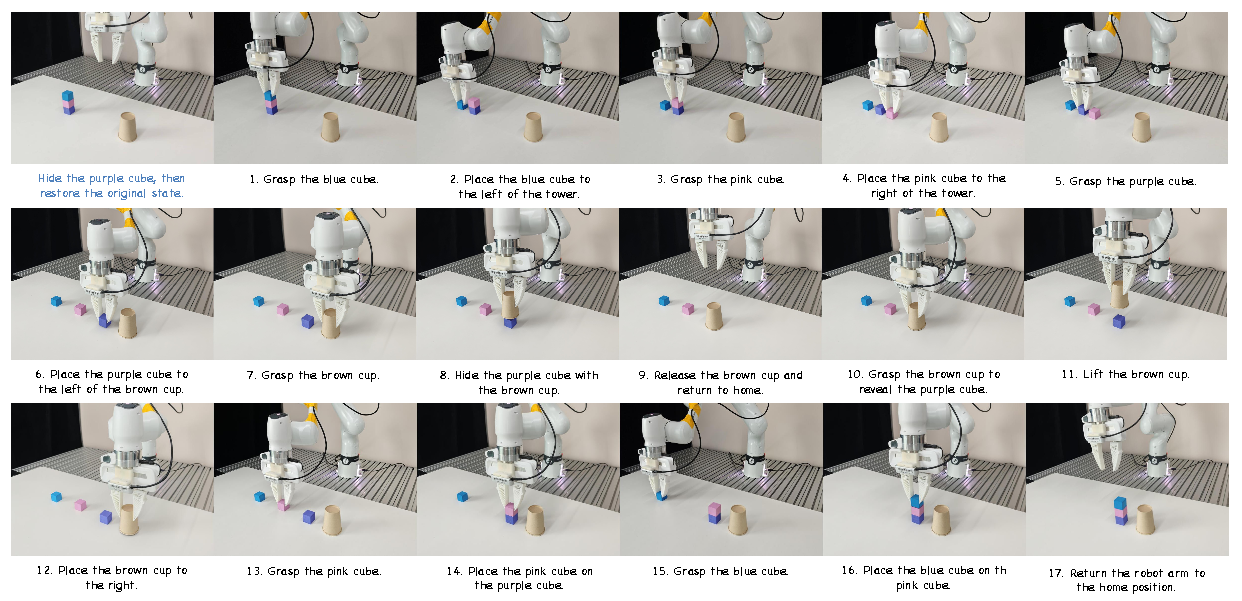
\includegraphics[width=1\textwidth]{Figures/appendix_realworld4.pdf} 
    \caption{\textbf{Long-horizon memorize and restore task (Occlusion).} A stress-test for causal memory retention. The robot sequentially hides the purple cube with a brown cup, performs intermediate tasks, and successfully recalls the hidden object's location to restore the original state.}
    \label{fig:appendix_step4}
\end{figure}


\subsubsection{Design of Simulation Tasks}
To comprehensively evaluate the capabilities of RoboStream, we carefully select and design tasks across two simulation platforms: SIMPLER~\cite{li2025evaluating} and RLBench~\cite{james2020rlbench}. Rather than treating all tasks uniformly, we deliberately categorize them into two distinct evaluation axes to independently stress-test zero-shot generalization, high-precision spatial grounding, and long-horizon causal memory.

\noindent\textbf{Evaluating Spatial Grounding and Zero-Shot Generalization.} 
The first suite of tasks is designed to isolate and evaluate the explicit 3D geometric grounding provided by STF-Tokens, independent of long-term memory requirements. To assess zero-shot cross-embodiment generalization, we deploy our framework in the SIMPLER benchmark (visualized in Fig.~\ref{fig:appendix_sim1}, top). We evaluate the Google Robot embodiment on tasks like ``Pick Coke Can'' and ``Move Near'', alongside the WidowX + Bridge embodiment on tasks such as ``Put Spoon on Towel'', ``Put Carrot on Plate'', ``Stack Green Block on Yellow Block'', and ``Put Eggplant in Basket''. The design rationale here is to verify that the spatio-temporal reasoning enabled by STF-Tokens is not overfitted to a specific robot kinematic structure or camera viewpoint. By deploying RoboStream on unseen embodiments without fine-tuning, we demonstrate its robustness to visual domain shifts and novel spatial layouts. 

Complementing this cross-embodiment evaluation, we select 15 diverse single-step tasks from the standard RLBench suite (e.g., \textit{Close Drawer, Lamp Off, Meat Off Grill, Put Rubbish in Bin, Slide Block to Target}, as shown in Fig.~\ref{fig:appendix_sim1}, bottom). The primary motivation for including these short-horizon tasks is their demand for fine-grained geometric understanding and contact-rich interactions. Testing on these specific scenarios allows us to prove that explicit 3D geometric representations—captured via centroids and Gaussian shapes—surpass pixel-level implicit reasoning even before complex sequential planning is required.

\noindent\textbf{Evaluating Causal Memory and Object Permanence.} 
To explicitly stress-test the Causal Spatio-Temporal Graph (CSTG) and its ability to maintain object permanence, we engineer a custom suite of 8 complex, long-horizon tasks in RLBench. These tasks are structured around two distinct guidance modalities to evaluate different aspects of persistent memory. The first category consists of goal-image guided tasks (\textit{Bridge Between Towers, Place Blocks in Two Containers (Normal/Hard), and Stack Three/Five Colors}, visualized in Fig.~\ref{fig:appendix_sim2}). In these scenarios, the robot must deduce the correct multi-step execution sequence from a visually complex target state. This design tests the model's capacity to maintain spatial coherence and track multiple object states simultaneously as the scene dynamically evolves. 

The second category introduces text-guided tasks (\textit{Cover Top/Bottom Block with Box, and Unstack then Stack Four Colors}, visualized in Fig.~\ref{fig:appendix_sim3}), which are specifically designed to evaluate causal memory under severe occlusion. By instructing the robot to hide a target object and subsequently restore the environment, we force the system to rely entirely on its episodic memory log rather than immediate visual perception. This task design acts as a rigorous stress test, proving the absolute necessity of the CSTG in preventing spatial hallucinations when visual evidence is temporarily lost.

\begin{figure}[htpb]
    \centering
    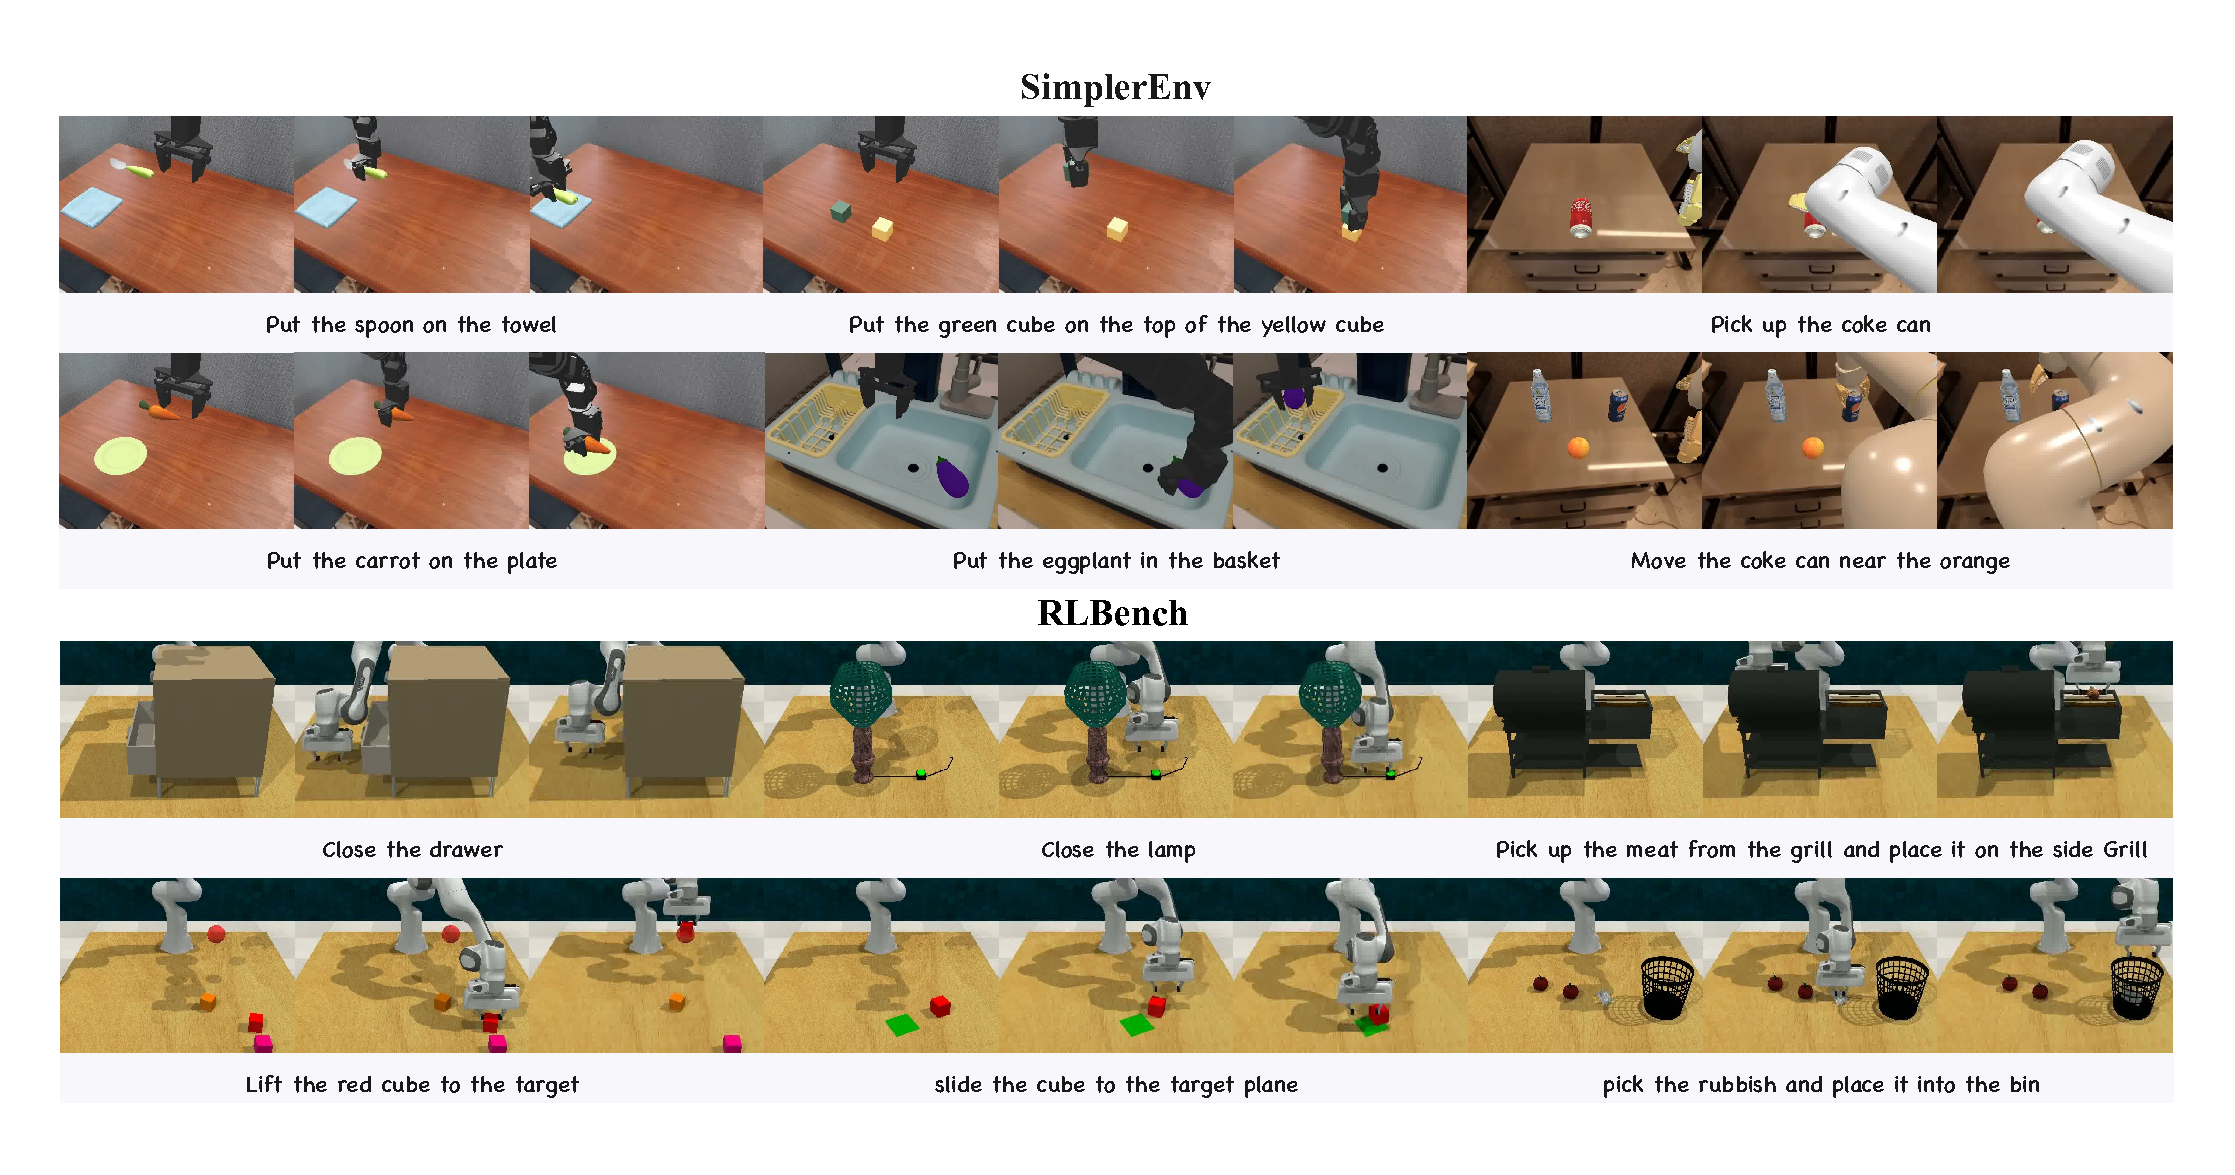
\includegraphics[width=1\textwidth]{Figures/RoboStream_Sim_OneStep.pdf} 
    \caption{\textbf{Visualization of Single-Step Evaluation Tasks.} Execution examples from the SIMPLER environment (top) and RLBench (bottom). These tasks are designed to demonstrate the model's zero-shot cross-embodiment generalization and its capability for high-precision spatial grounding in contact-rich scenarios.}
    \label{fig:appendix_sim1}
\end{figure}

\begin{figure}[htpb]
    \centering
    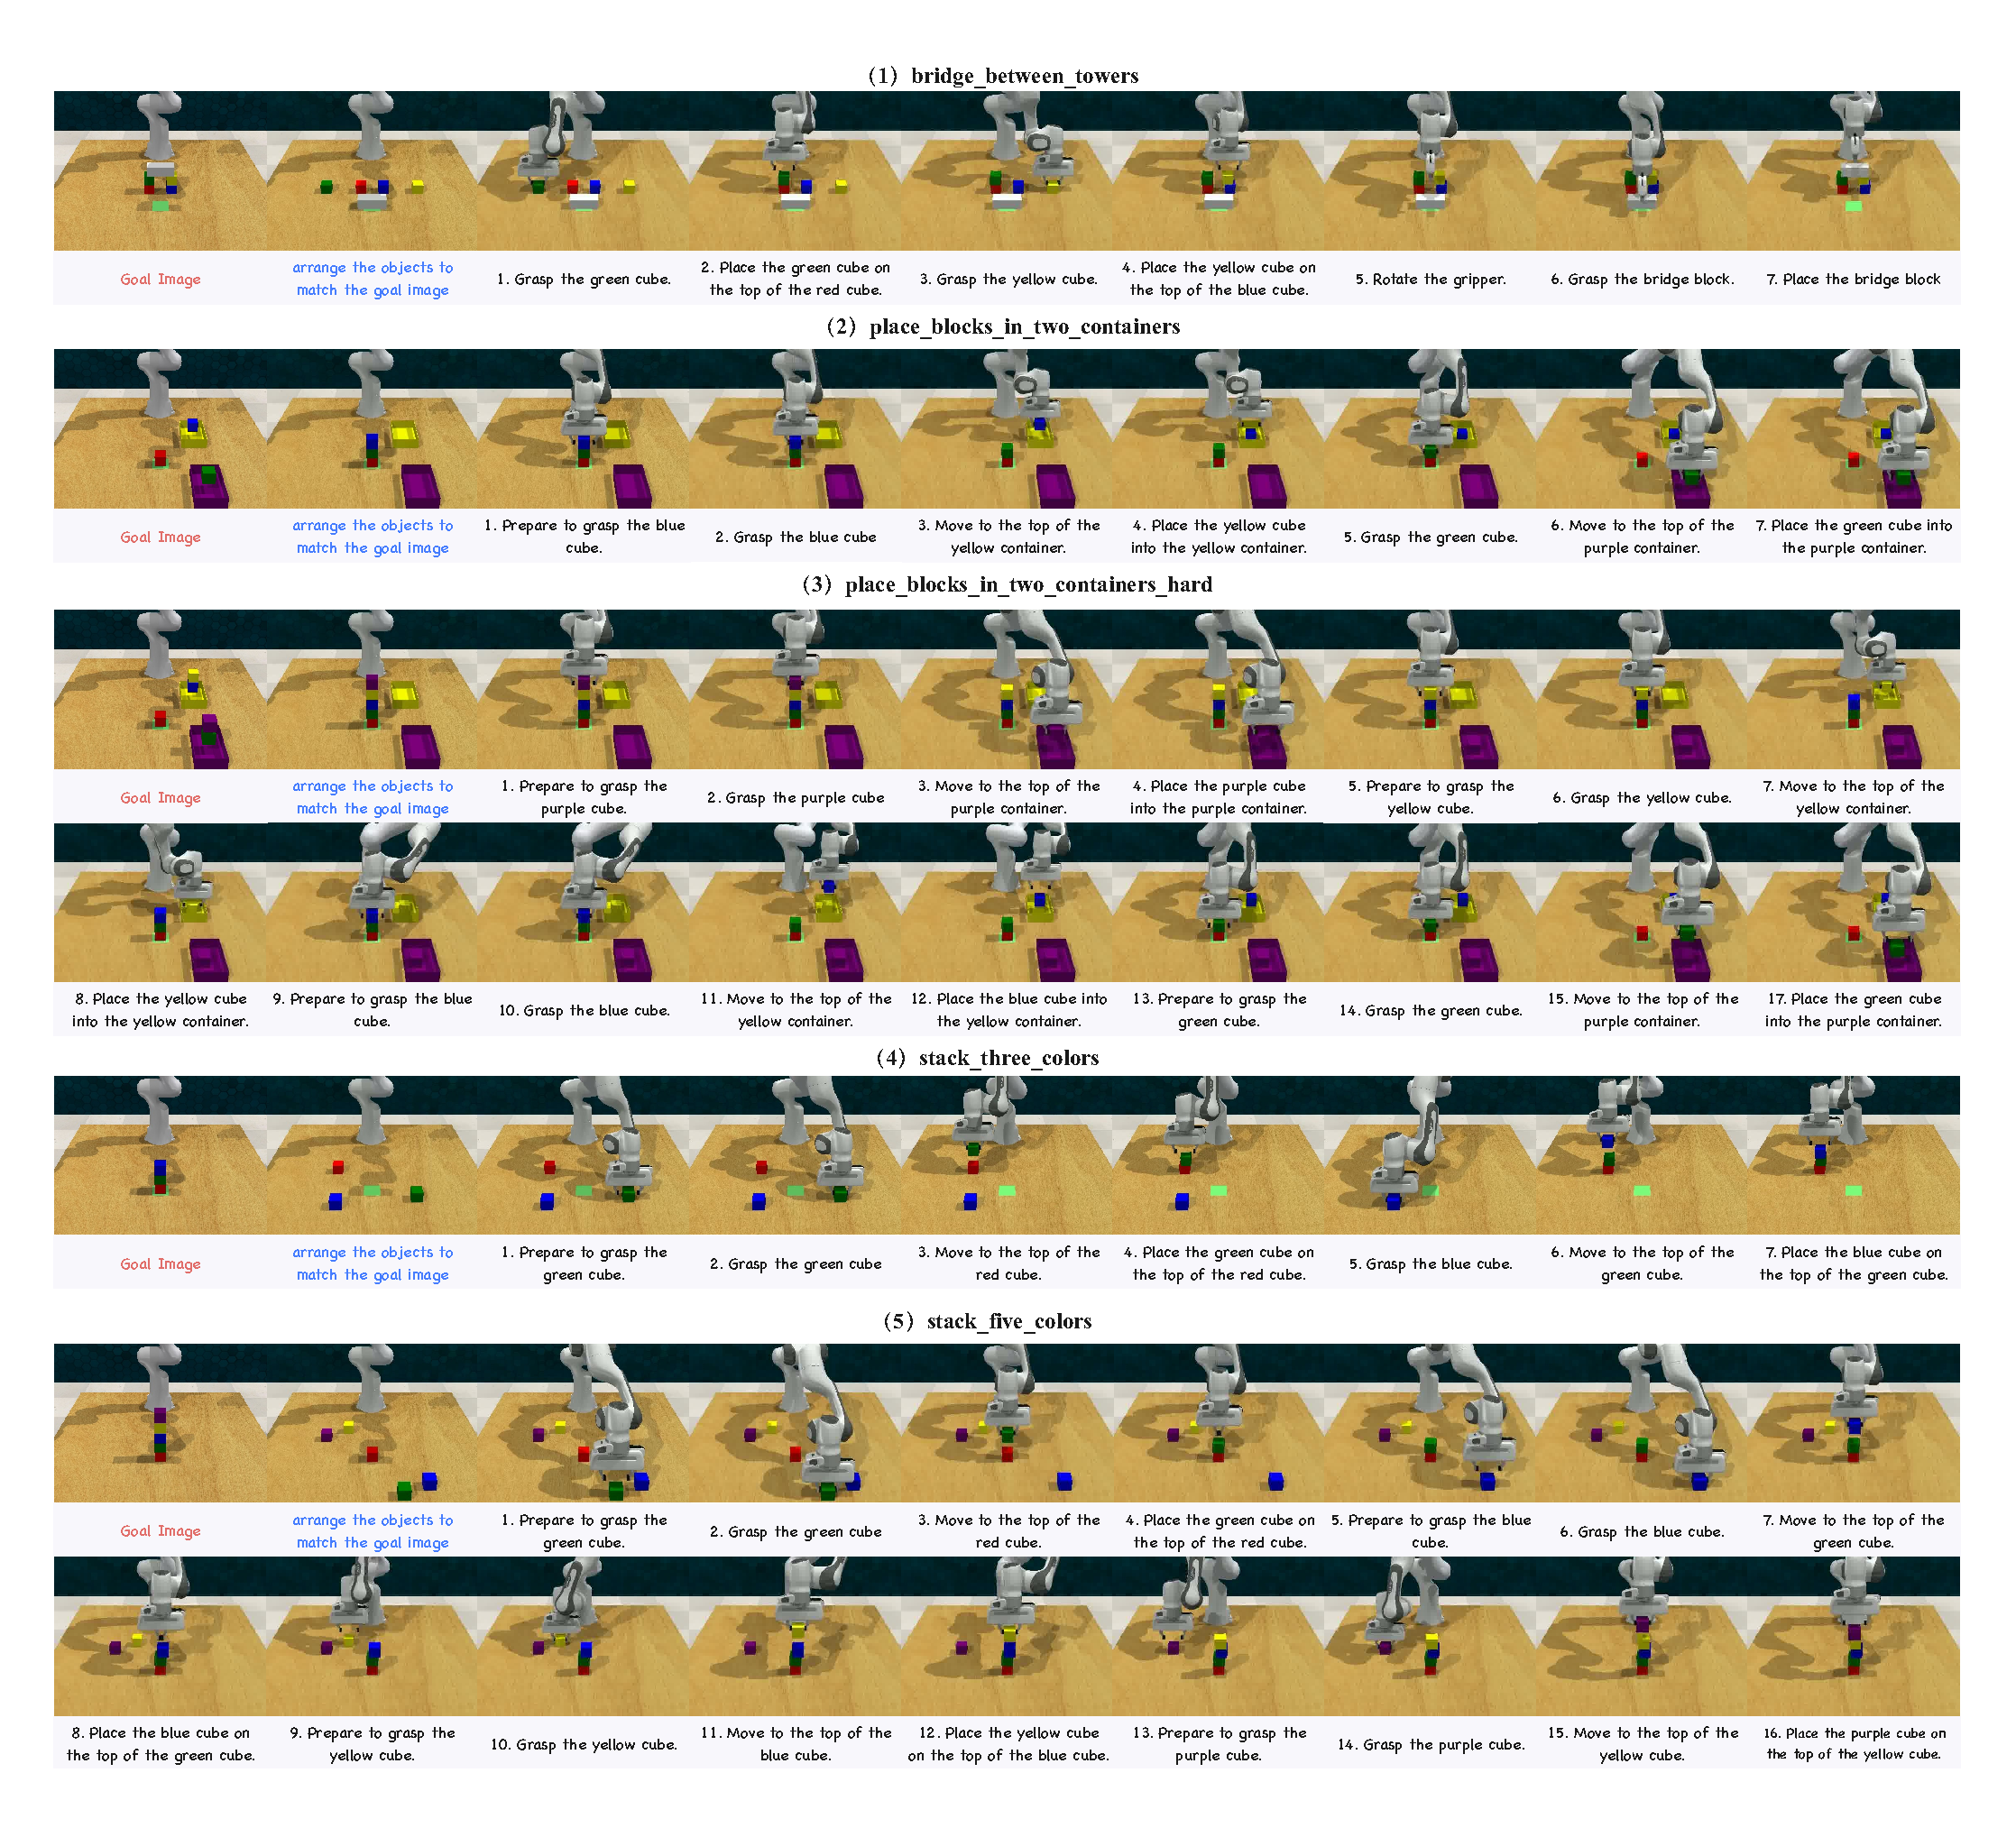
\includegraphics[width=1\textwidth]{Figures/RoboStream_MultiStep_Goal_Img.pdf} 
    \caption{\textbf{Goal-Image Guided Multi-Step Tasks.} Execution sequences for five long-horizon tasks in RLBench where the target state is provided via a visual goal image. These tasks systematically evaluate the model's ability to maintain spatial coherence and track multiple objects across extended dynamic trajectories.}
    \label{fig:appendix_sim2}
\end{figure}

\begin{figure}[htpb]
    \centering
    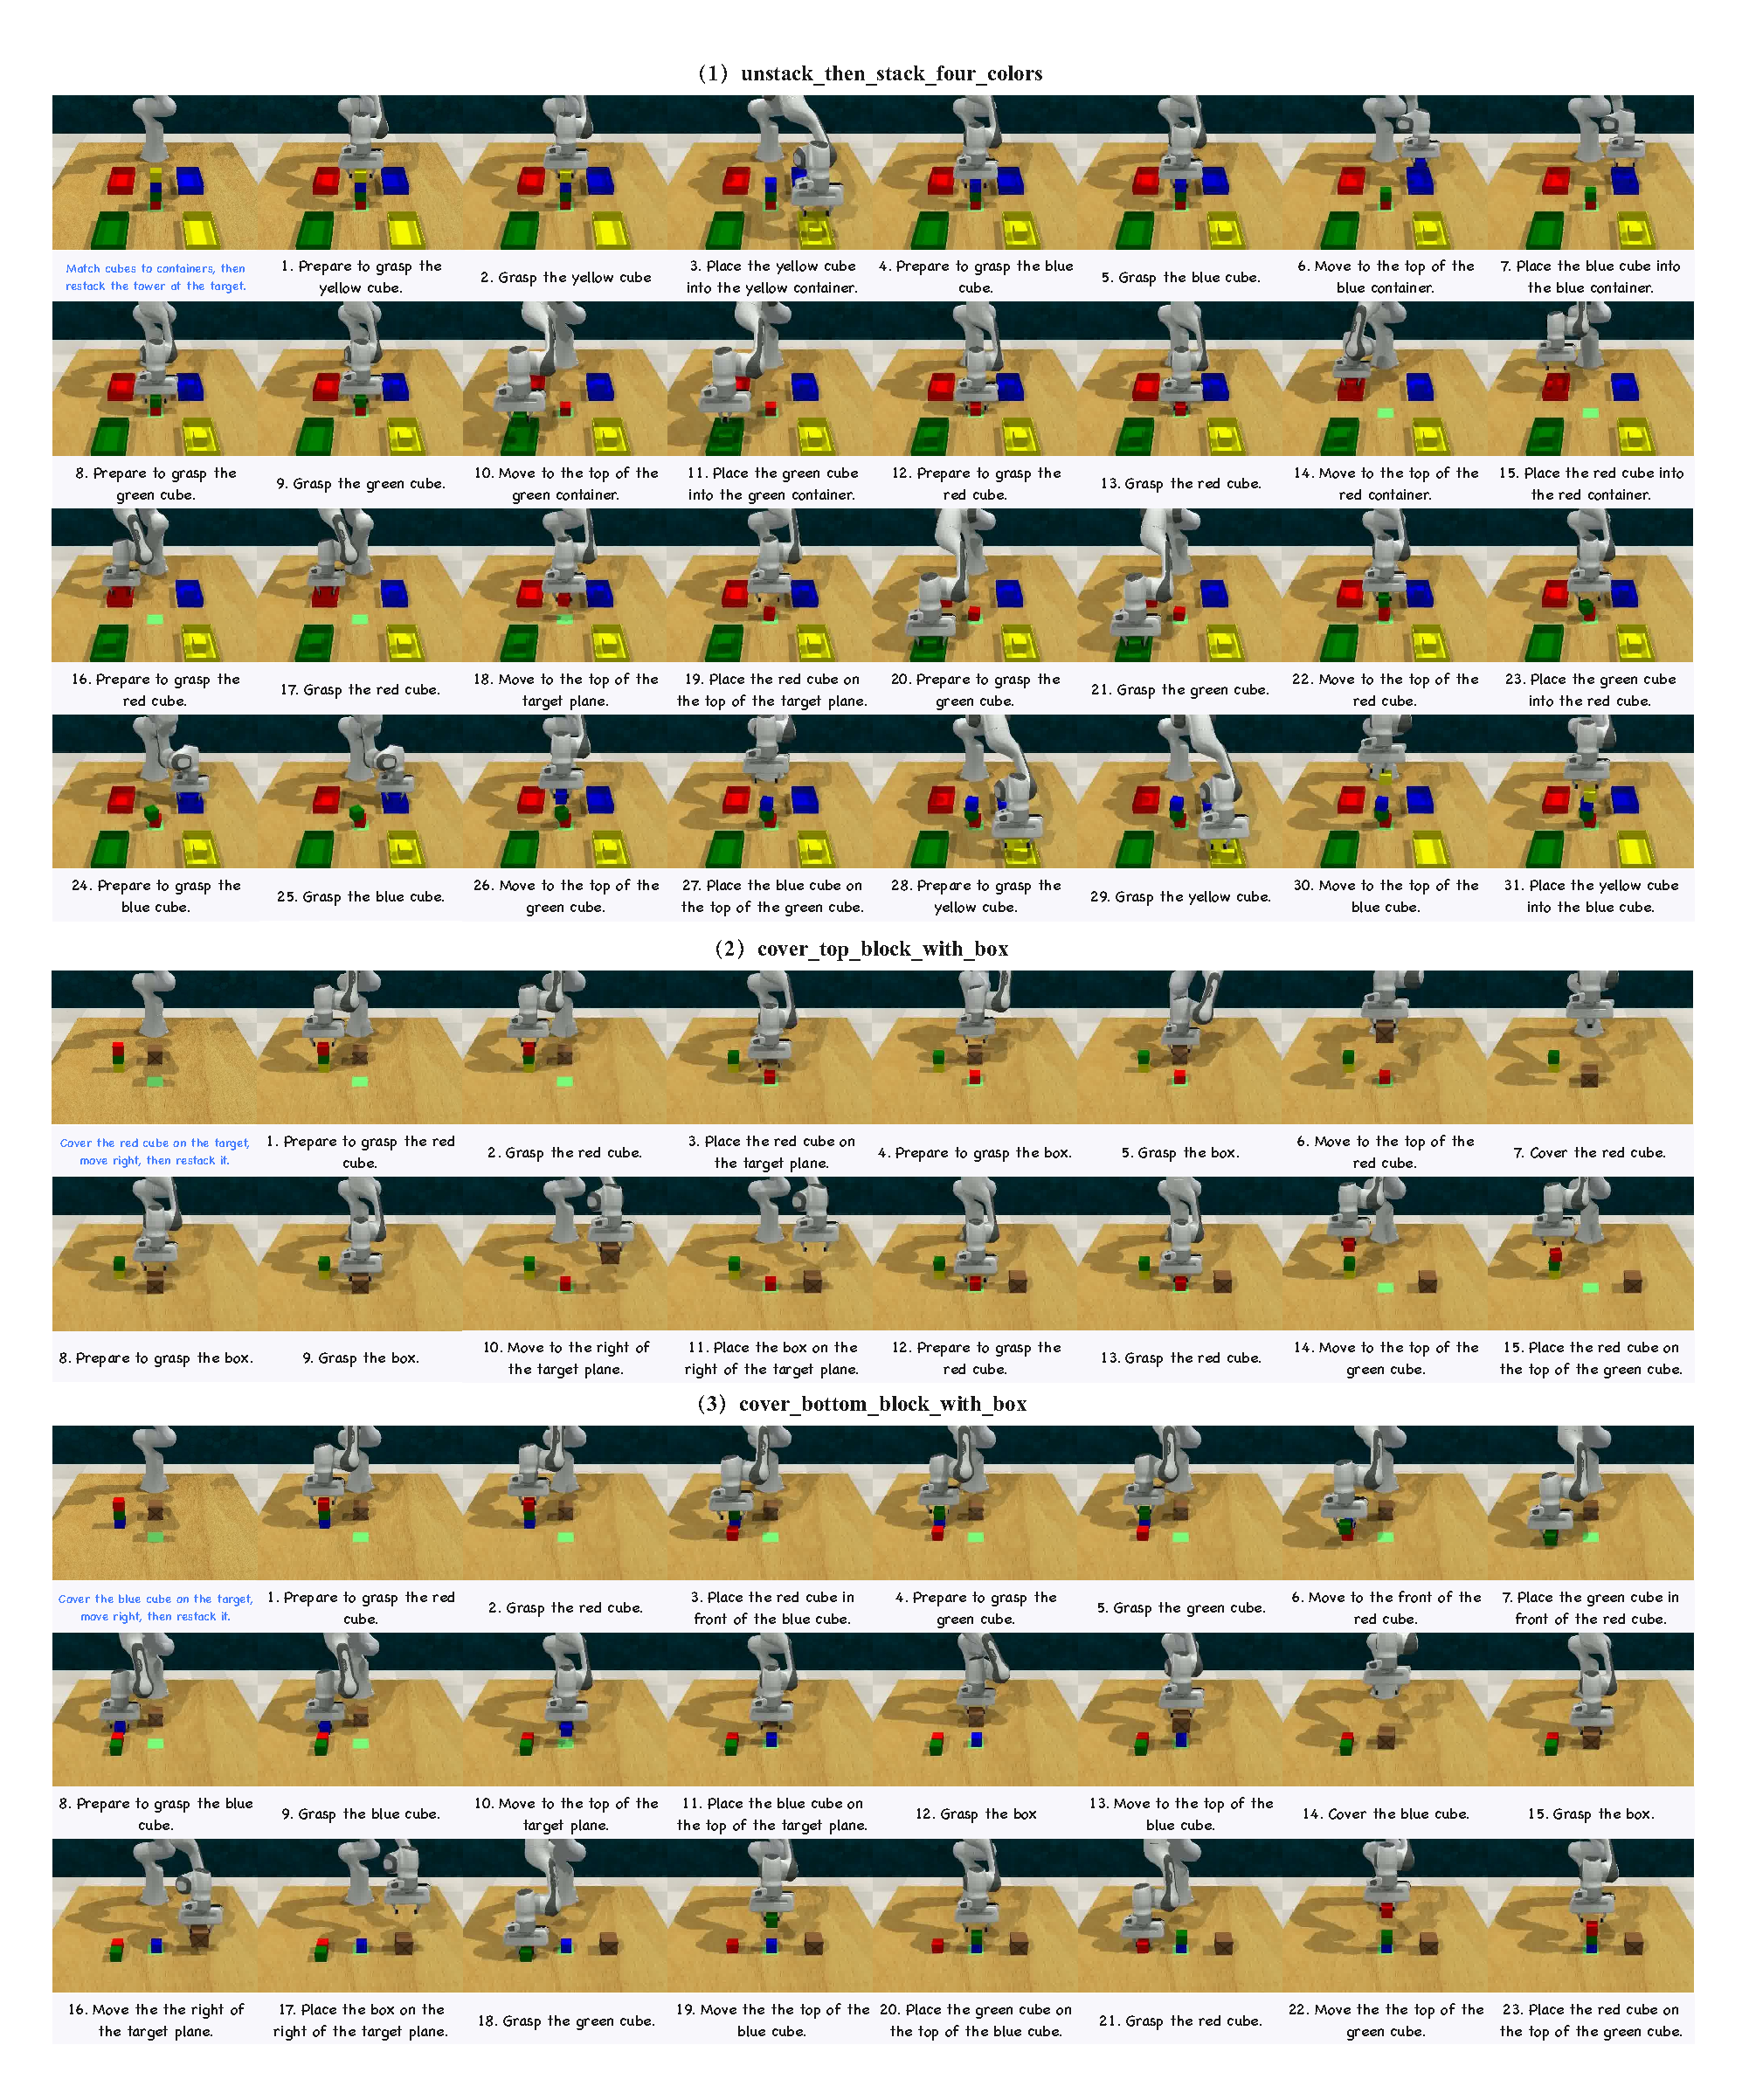
\includegraphics[width=1\textwidth]{Figures/RoboStream_MultiStep_Text.pdf} 
    \caption{\textbf{Text-Guided Multi-Step Tasks.} Execution sequences for three complex long-horizon tasks in RLBench driven by natural language instructions. Notably, tasks involving covering and revealing blocks rigorously stress-test the Causal Spatio-Temporal Graph (CSTG) for object permanence and causal memory retention under severe occlusion.}
    \label{fig:appendix_sim3}
\end{figure}

\subsection{Detailed Experimental Results}
\subsubsection{Detailed Results of Real-World Manipulation}
\begin{table}[htbp]
    \centering
    % \caption{\textbf{Detailed quantitative results of real-world tasks.} For Block Building and Disassembly, the \textit{Task} column shows the \textbf{goal state} to be achieved. For the Memorize \& Restore task, it instead shows the \textbf{initial scene state} paired with a text instruction, since the objective is to restore the scene after a hidden manipulation sequence.}
    \caption{\textbf{Detailed quantitative results of real-world tasks.}}
    \label{tab:real_world_detailed}
    \renewcommand{\arraystretch}{1.1} 
    \resizebox{\textwidth}{!}{
    \begin{tabular}{m{0.3\textwidth} c c c c c c}
        \toprule
        % 使用 multirow 和 multicolumn 将“任务属性”和“模型成功率”在视觉上彻底分开
        \multirow{2}{*}{\textbf{Task}} & \multirow{2}{*}{\textbf{Difficulty}} & \multicolumn{5}{c}{\textbf{Success Rate}} \\
        \cmidrule(lr){3-7}
        & & \textbf{SoFar} & \textbf{VoxPoser} & \textbf{RoboStream-8B} & \textbf{RoboStream-32B} & \textbf{RoboStream-235B} \\
        \midrule
        
        % ==================== Section 1: 搭积木 ====================
        \multicolumn{7}{c}{\textit{Block Building (Bottom-to-Top)} {\scriptsize $\vert$ \textit{Task $=$ Goal Image}}} \\
        \midrule
        \begin{minipage}{0.3\textwidth}
            \centering \vspace{1pt}
            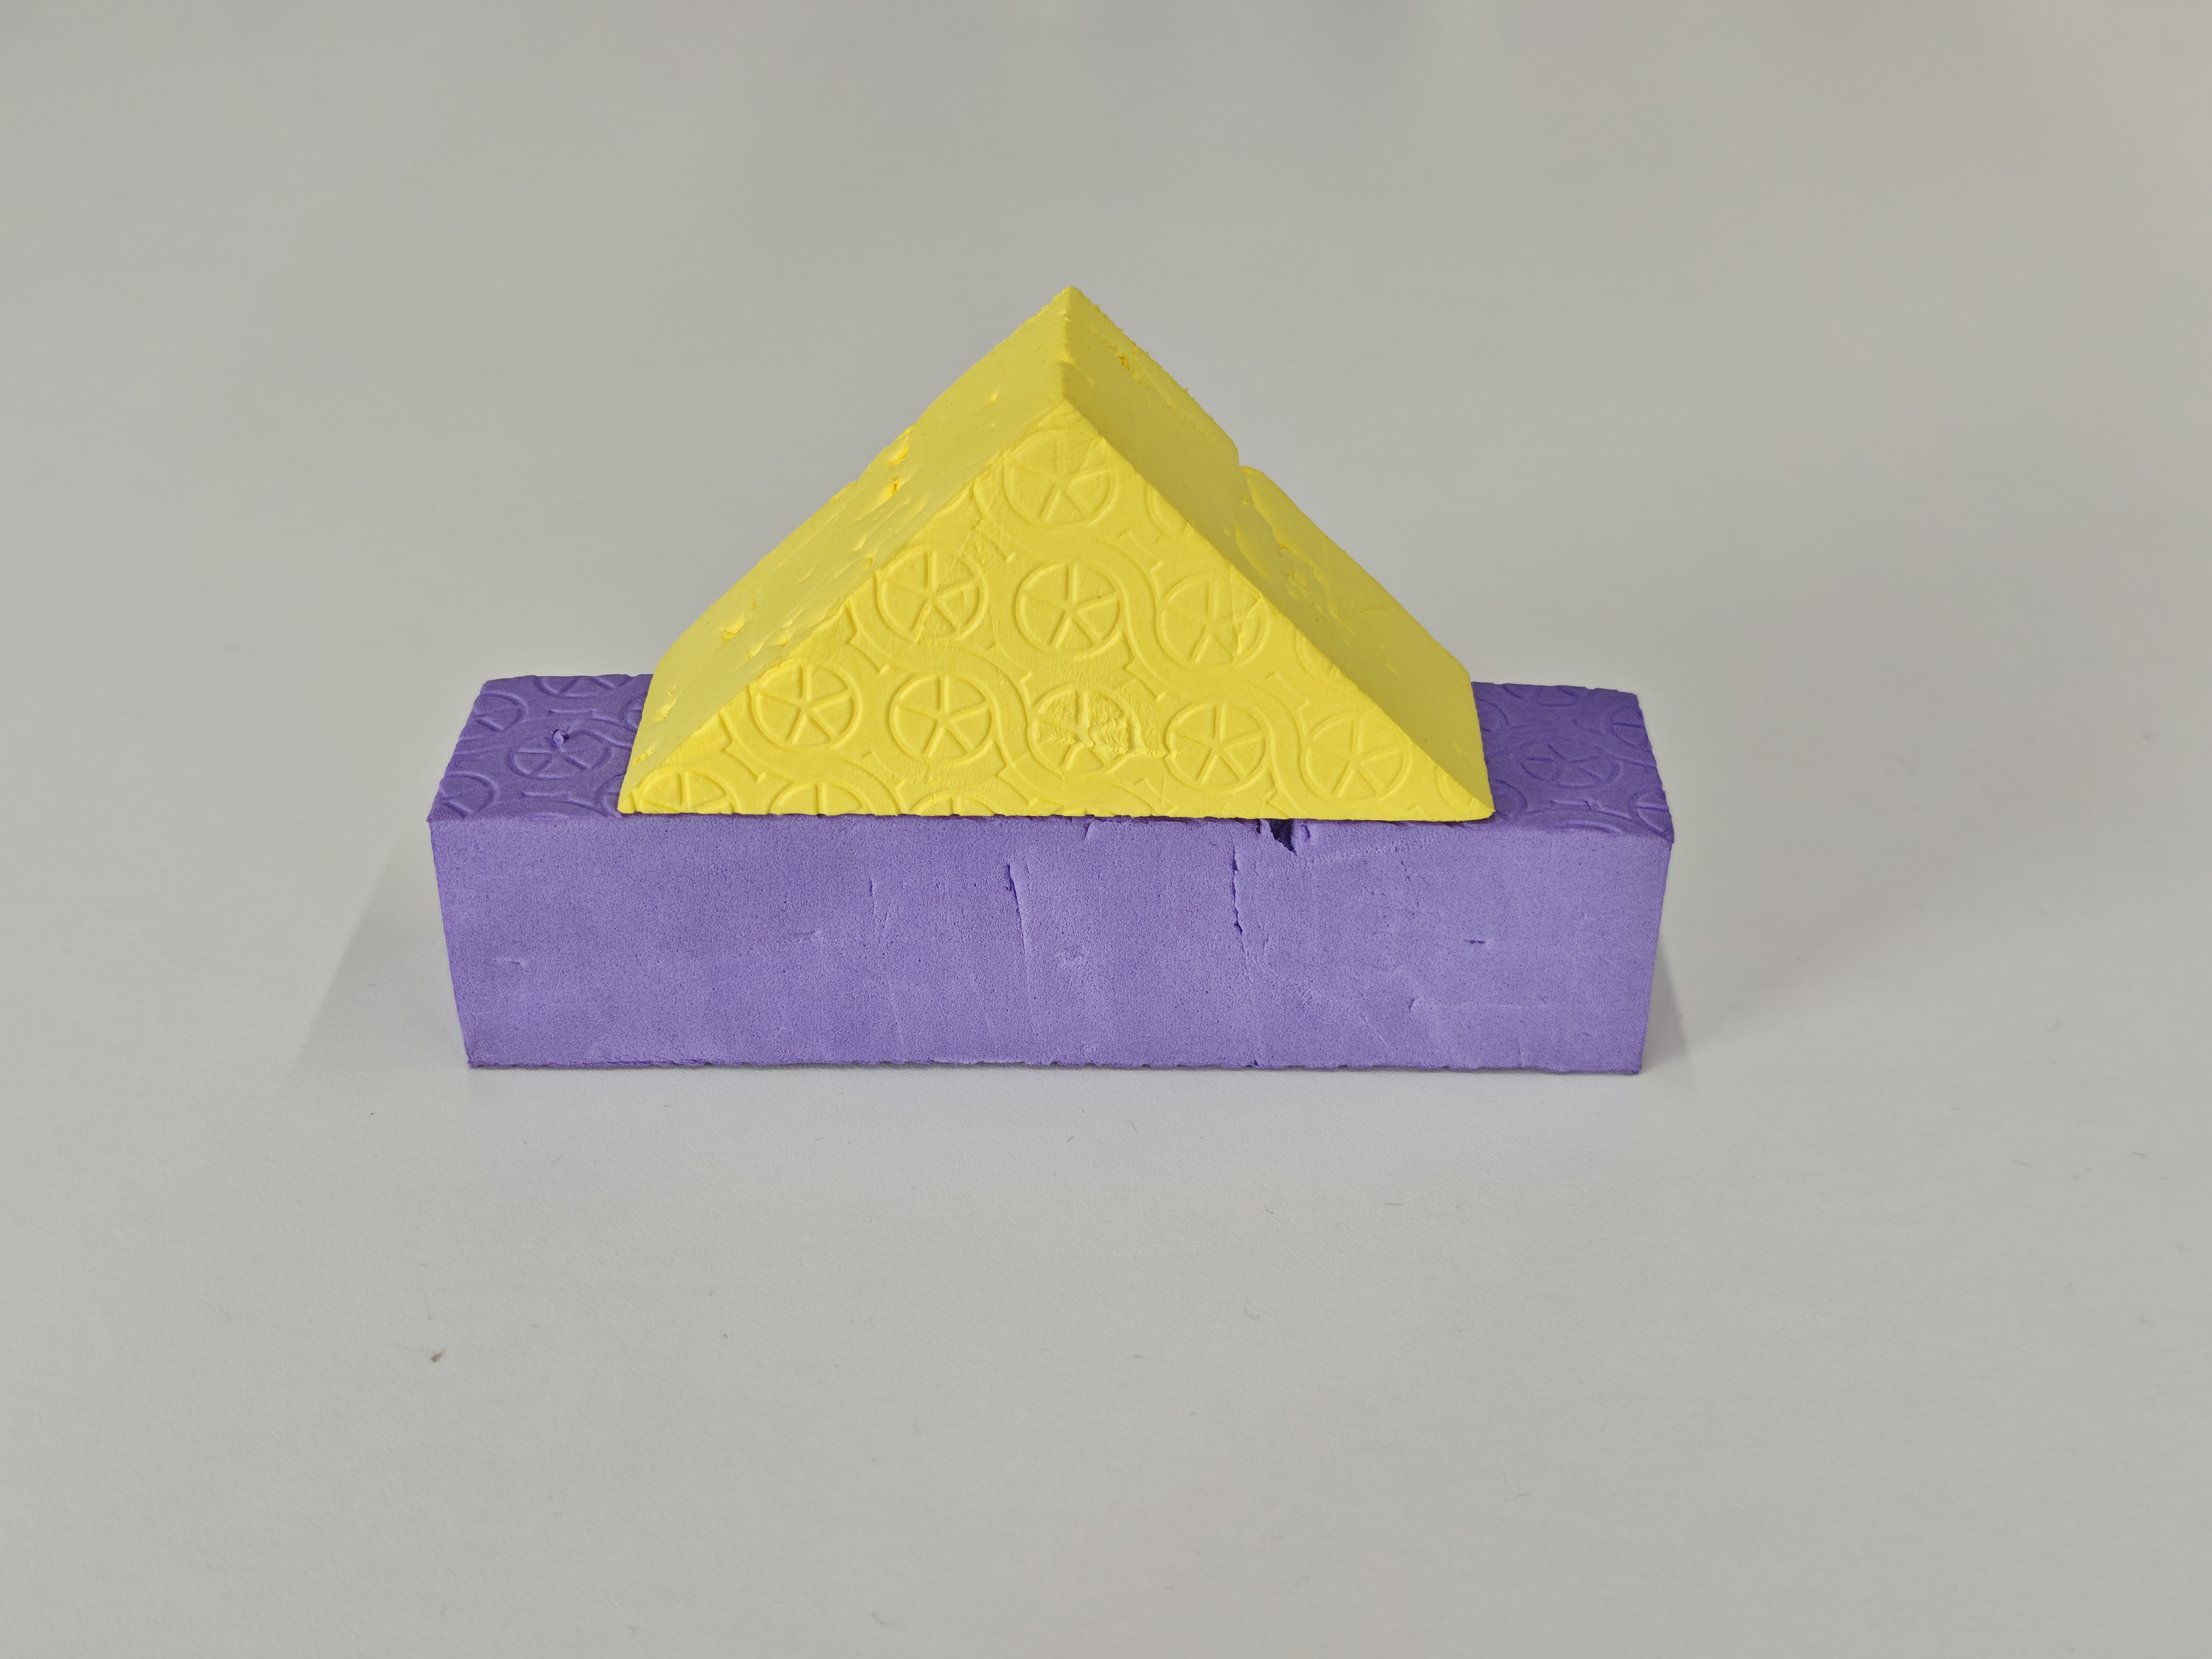
\includegraphics[height=1.0cm]{Figures/goal_images/easy1.jpg}
            \vspace{1pt}
        \end{minipage} 
        & Easy & 3/3 & 2/3 & 1/3 & 2/3 & \textbf{2/3} \\
        
        \begin{minipage}{0.3\textwidth}
            \centering \vspace{1pt}
            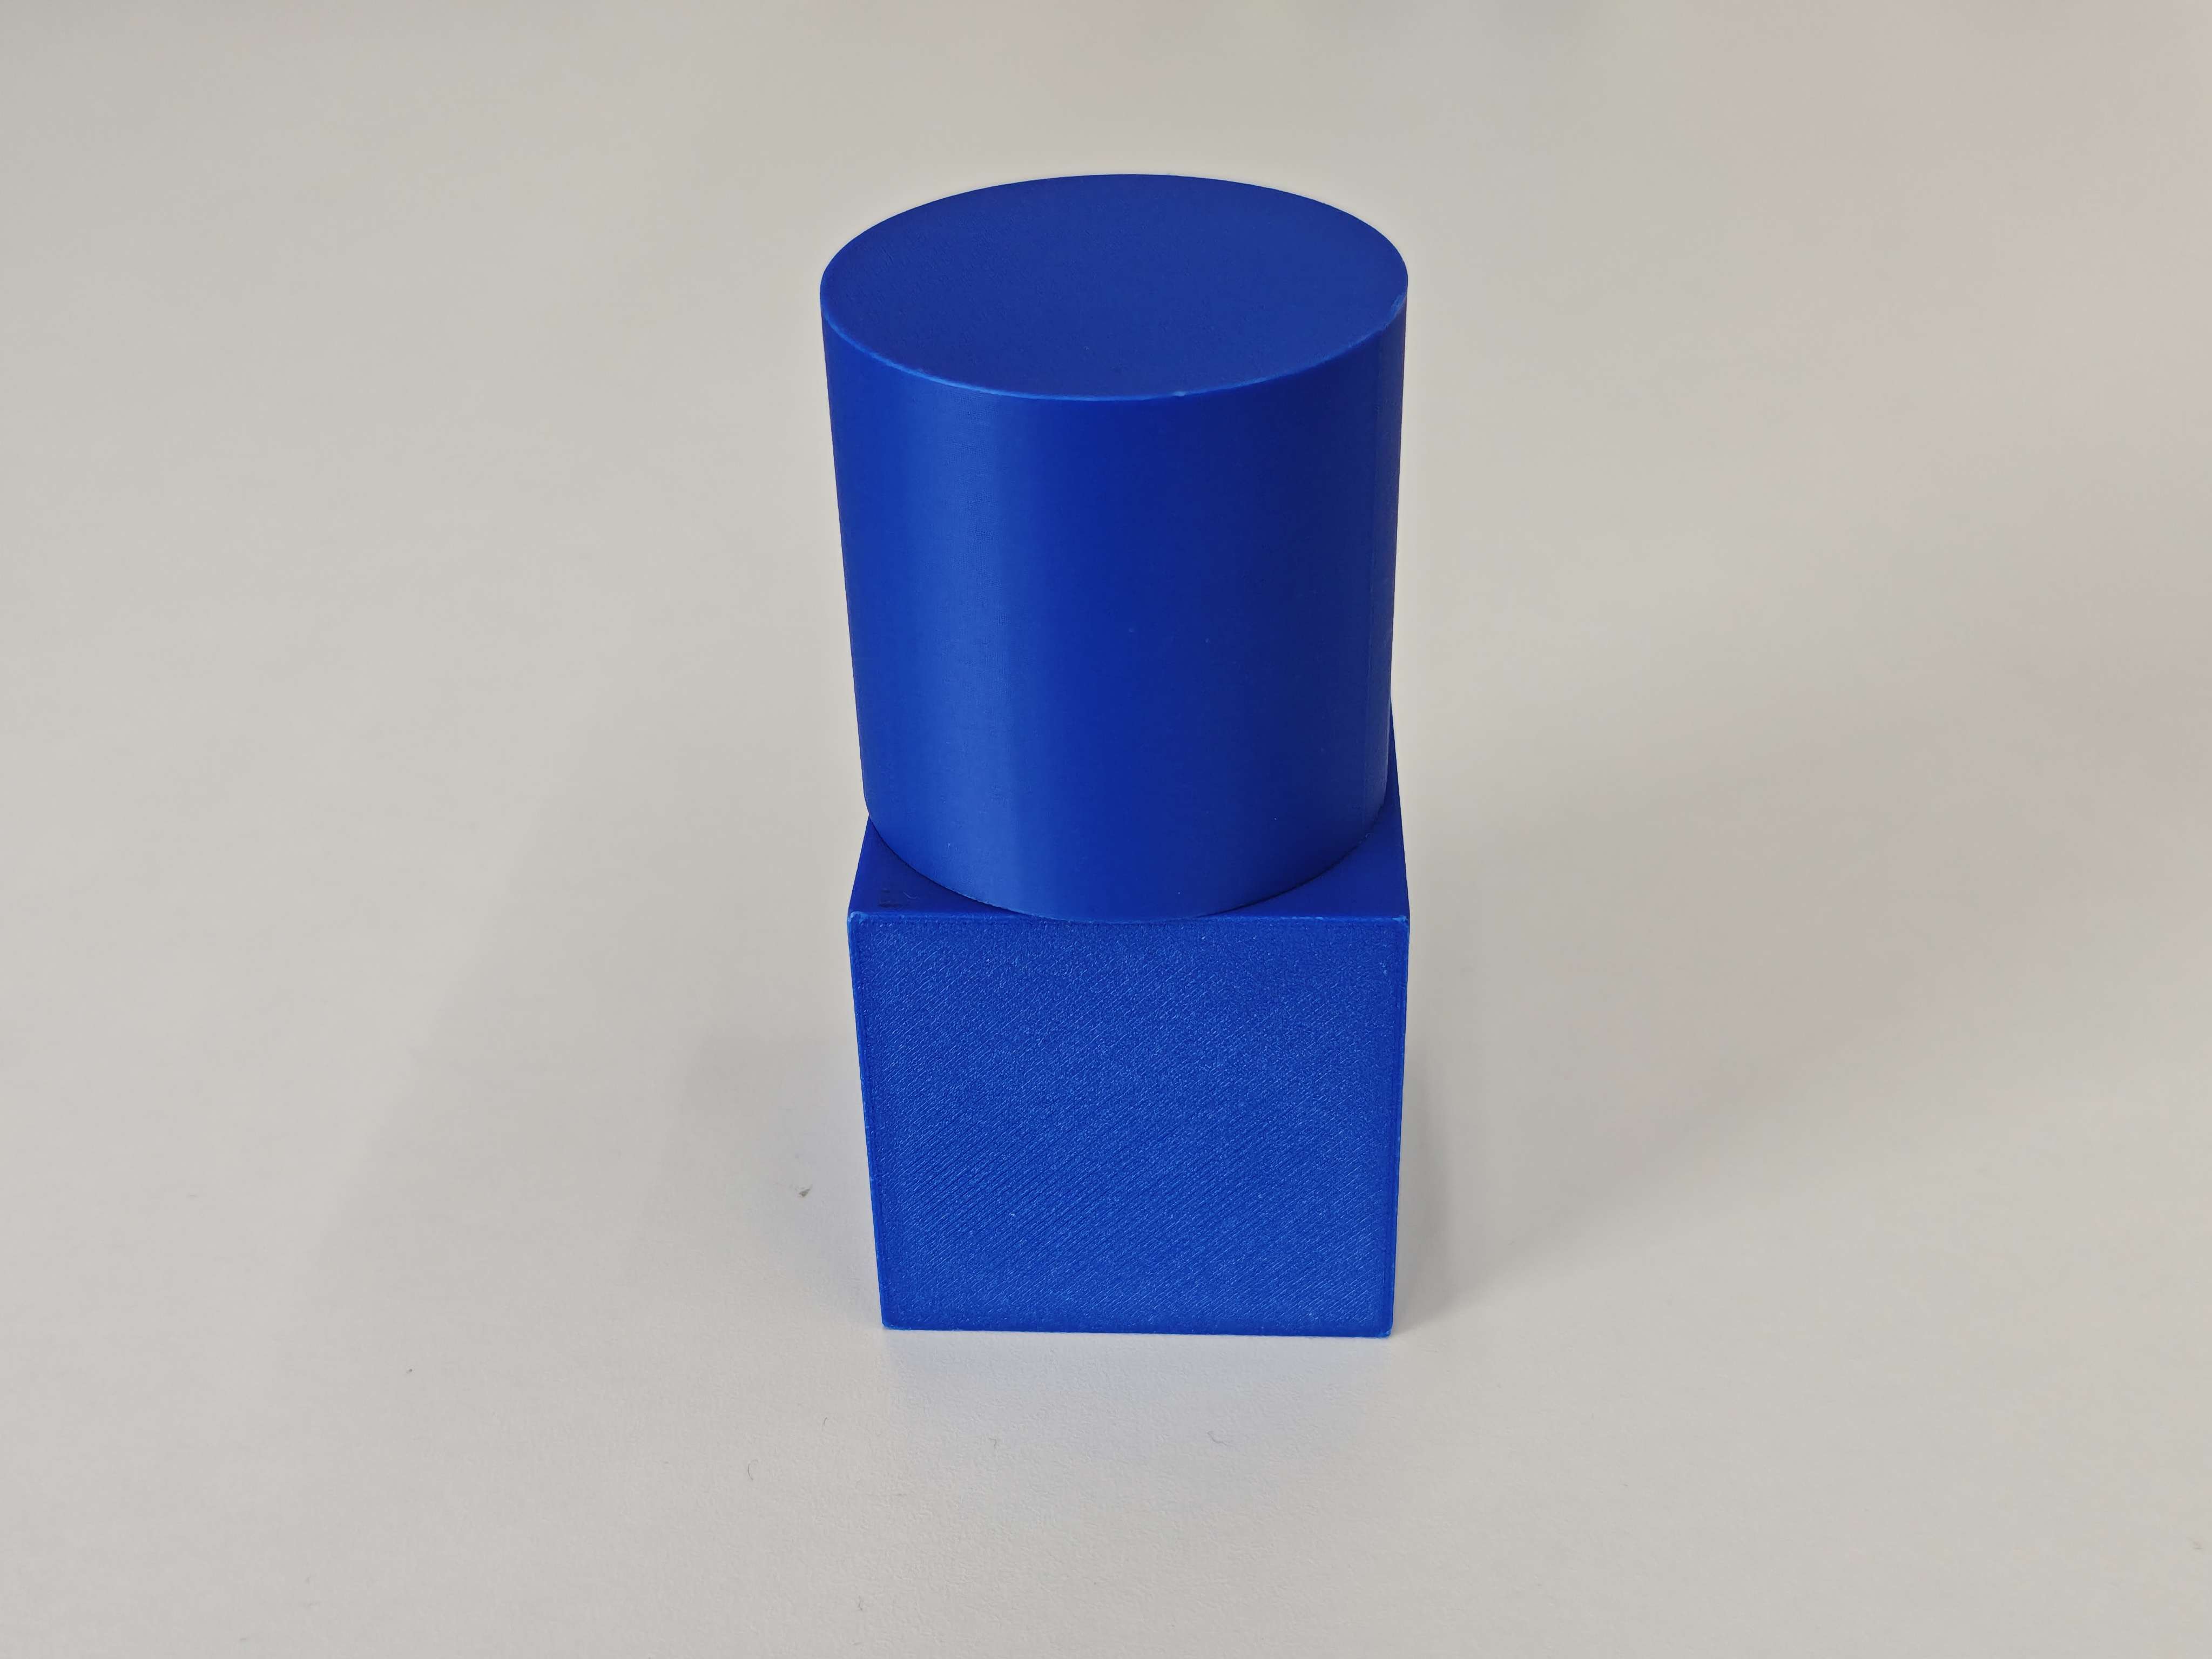
\includegraphics[height=1.0cm]{Figures/goal_images/easy2.jpg}
            \vspace{1pt}
        \end{minipage} 
        & Easy & 2/3 & 2/3 & 3/3 & 1/3 & \textbf{3/3} \\
        
        \begin{minipage}{0.3\textwidth}
            \centering \vspace{1pt}
            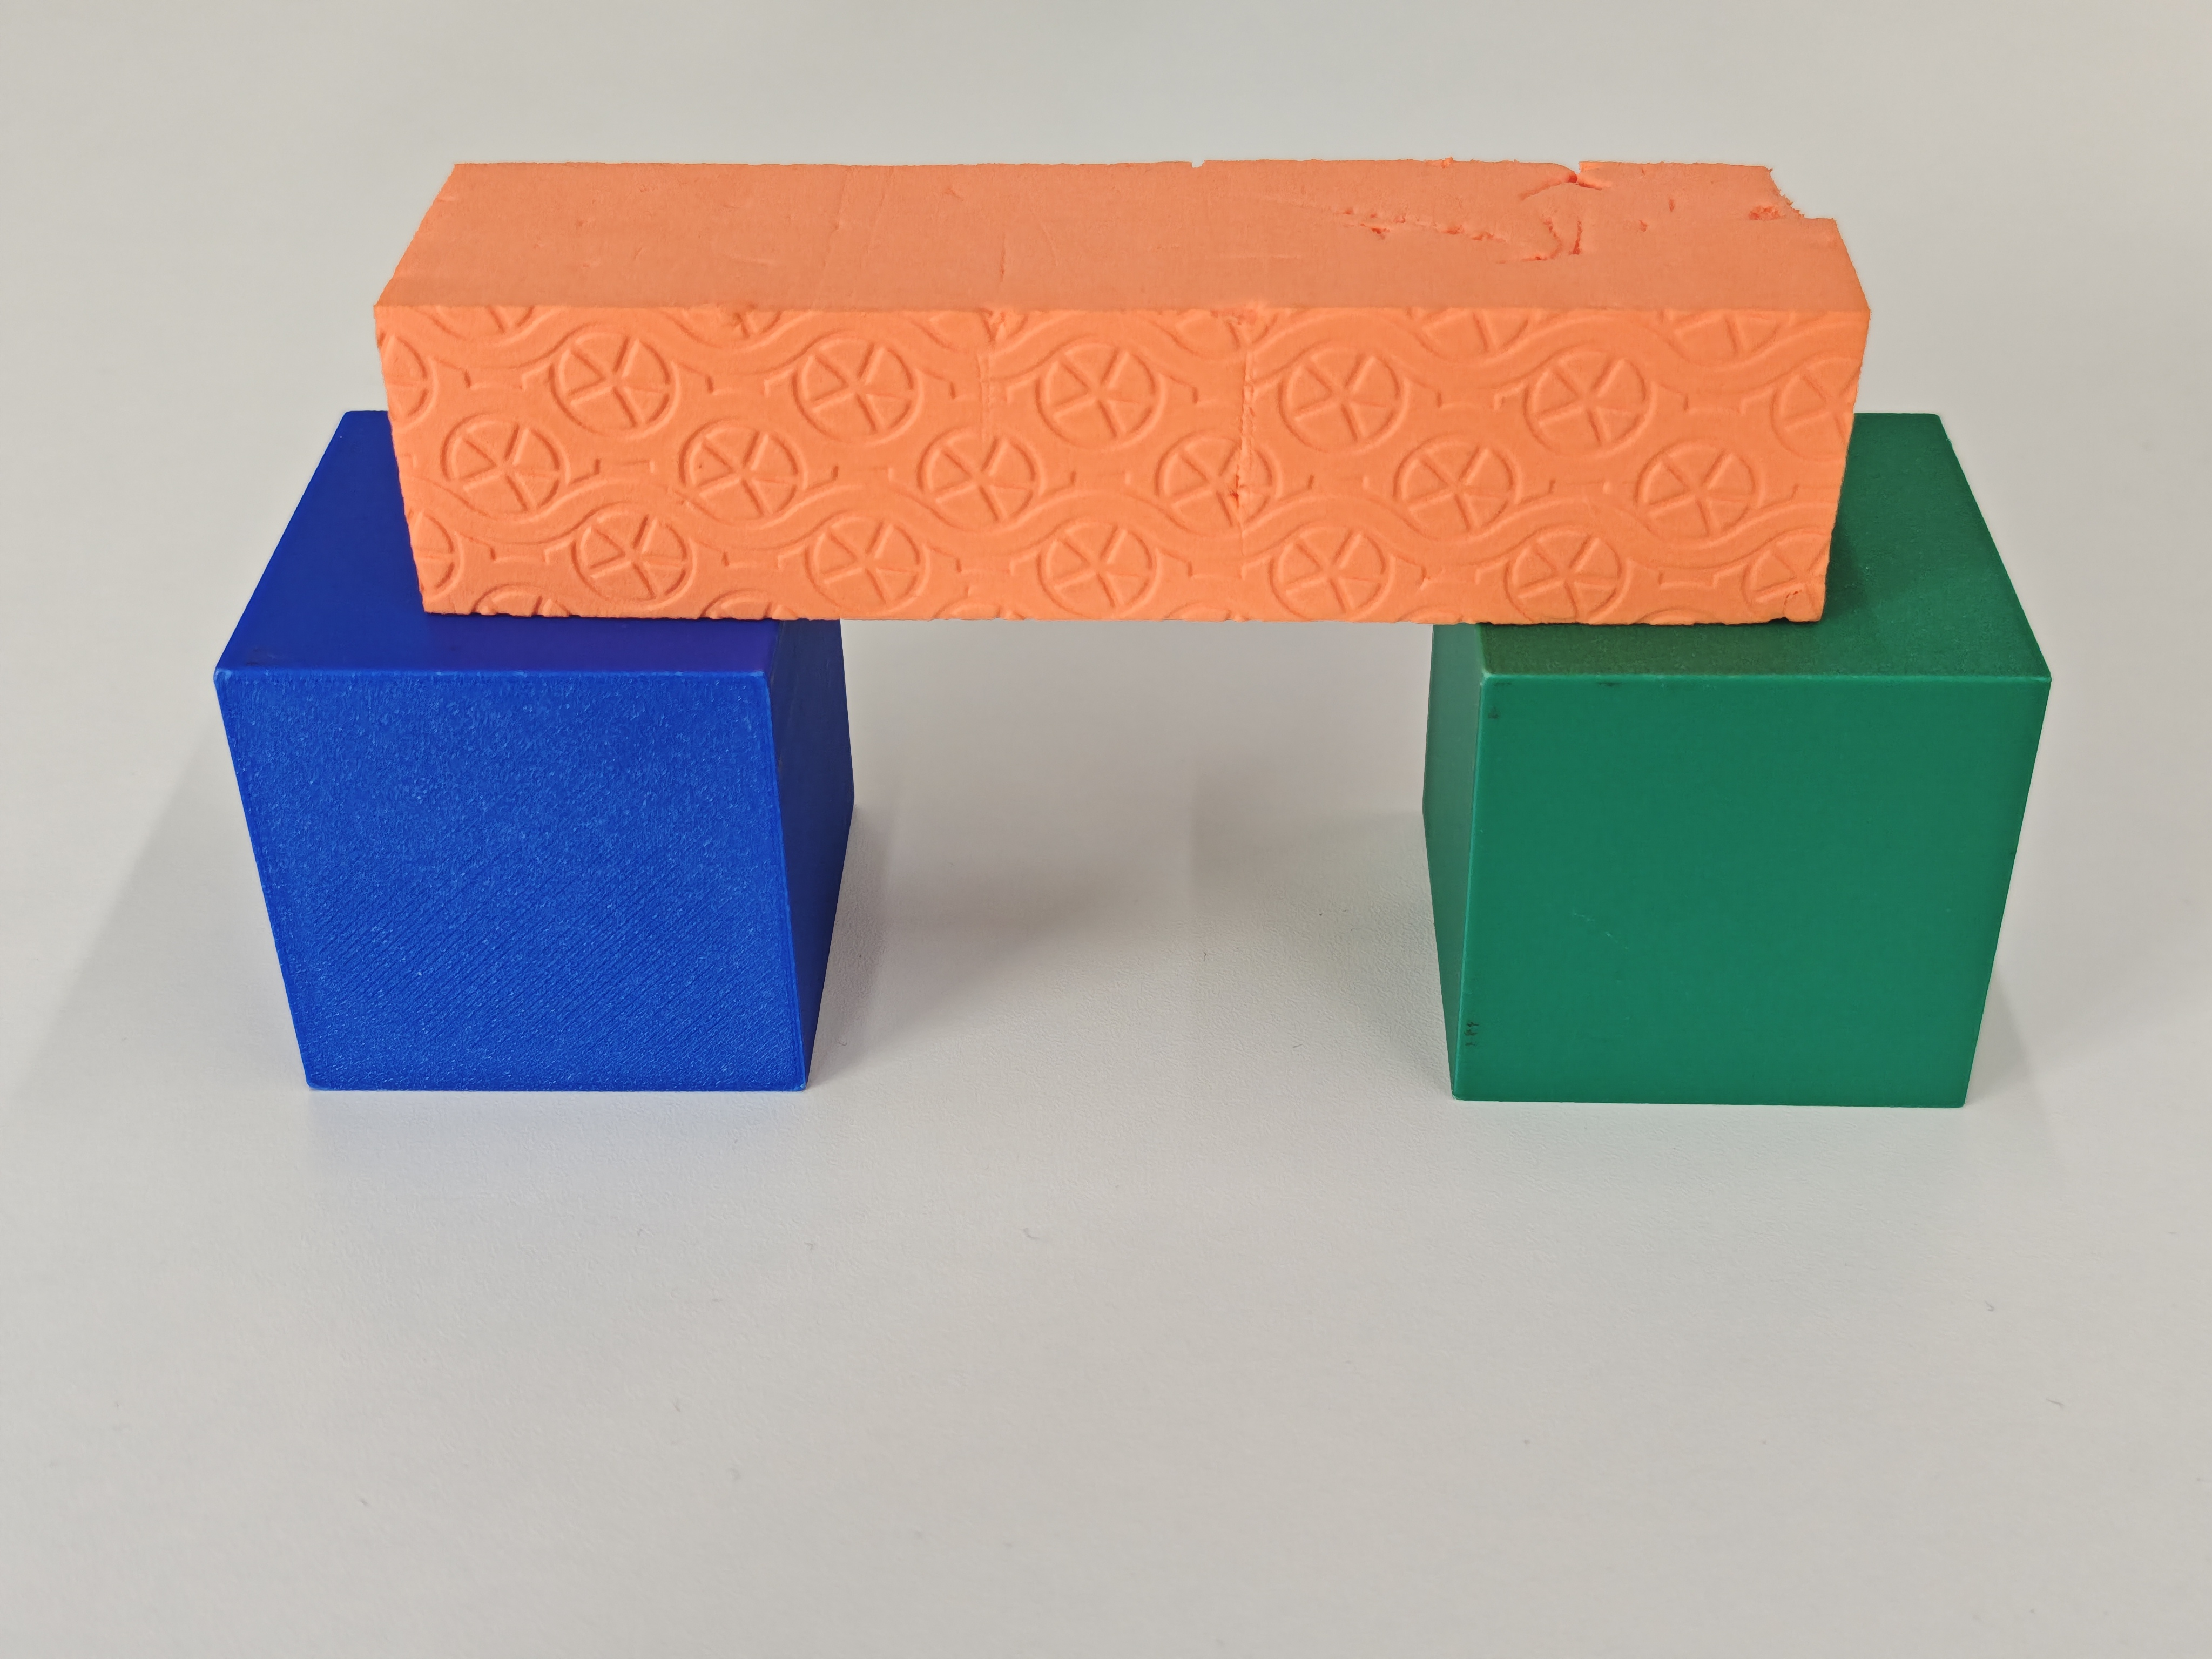
\includegraphics[height=1.0cm]{Figures/goal_images/easy3.jpg}
            \vspace{1pt}
        \end{minipage} 
        & Easy & 0/3 & 0/3 & 1/3 & 3/3 & \textbf{2/3} \\
        
        \begin{minipage}{0.3\textwidth}
            \centering \vspace{1pt}
            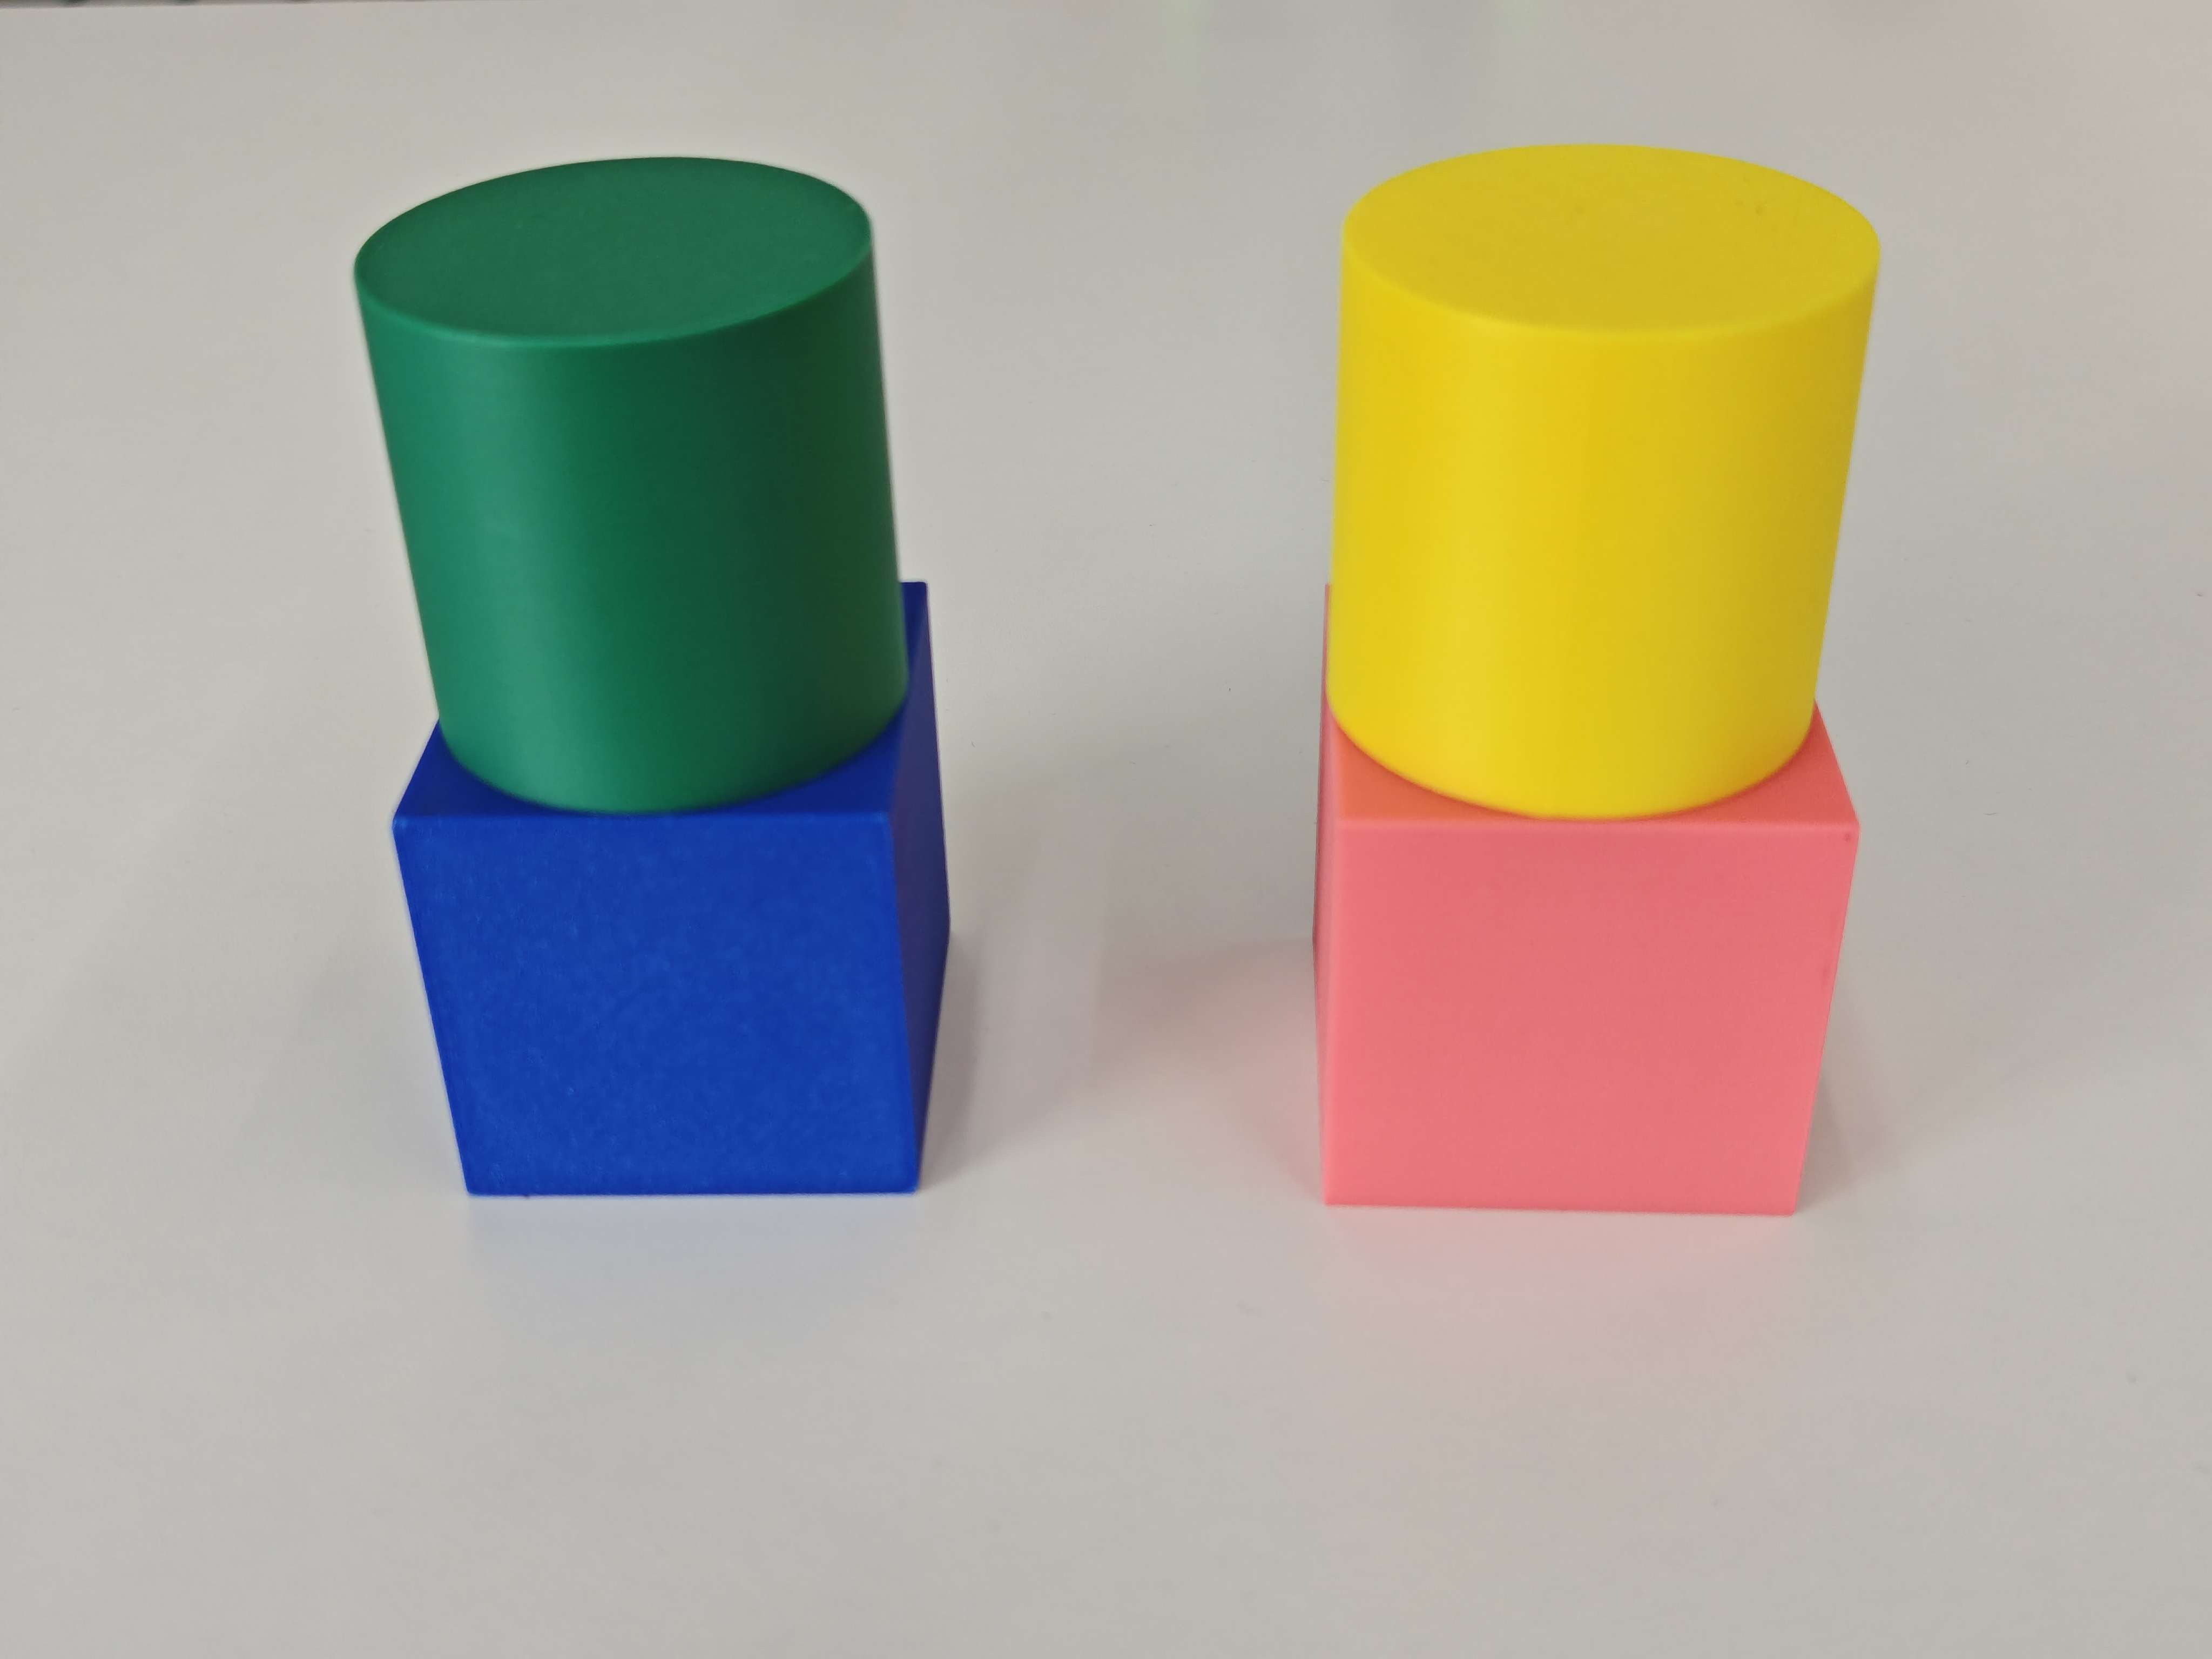
\includegraphics[height=1.0cm]{Figures/goal_images/medium1.jpg}
            \vspace{1pt}
        \end{minipage} 
        & Medium & 0/3 & 2/3 & 2/3 & 2/3 & \textbf{3/3} \\
        
        \begin{minipage}{0.3\textwidth}
            \centering \vspace{1pt}
            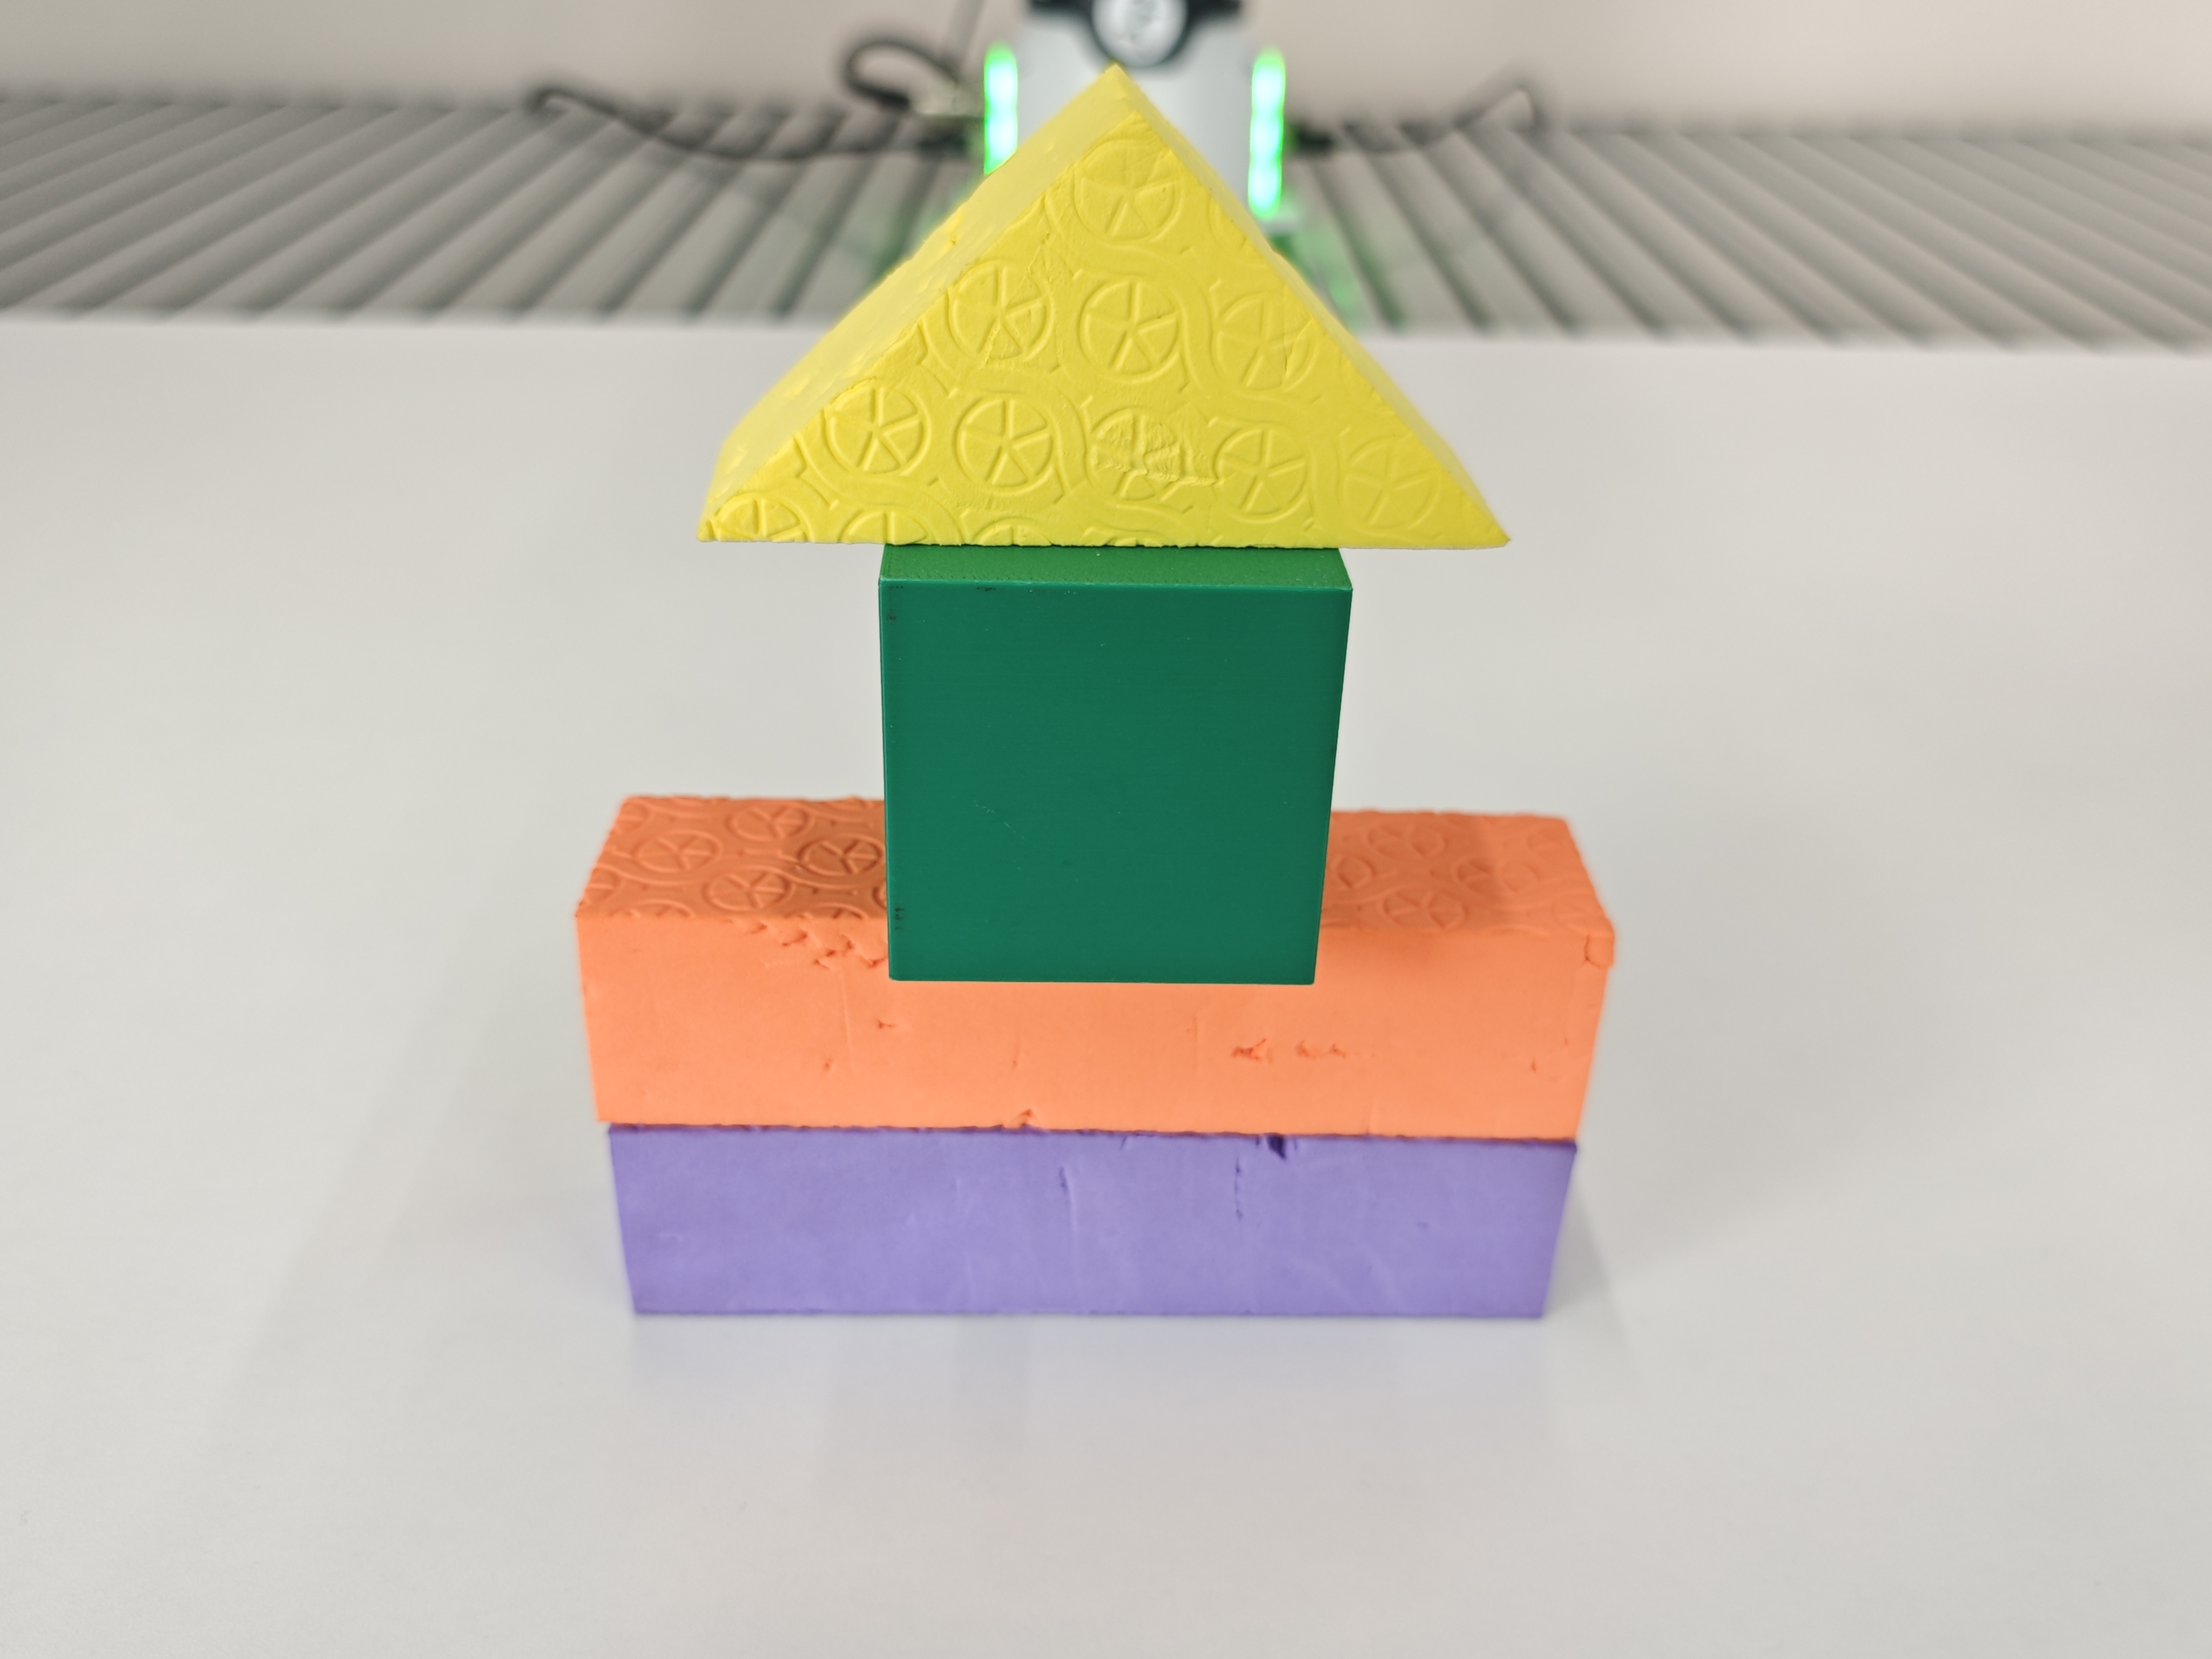
\includegraphics[height=1.0cm]{Figures/goal_images/medium2.jpg}
            \vspace{1pt}
        \end{minipage} 
        & Medium & 0/3 & 0/3 & 0/3 & 1/3 & \textbf{1/3} \\
        
        \begin{minipage}{0.3\textwidth}
            \centering \vspace{1pt}
            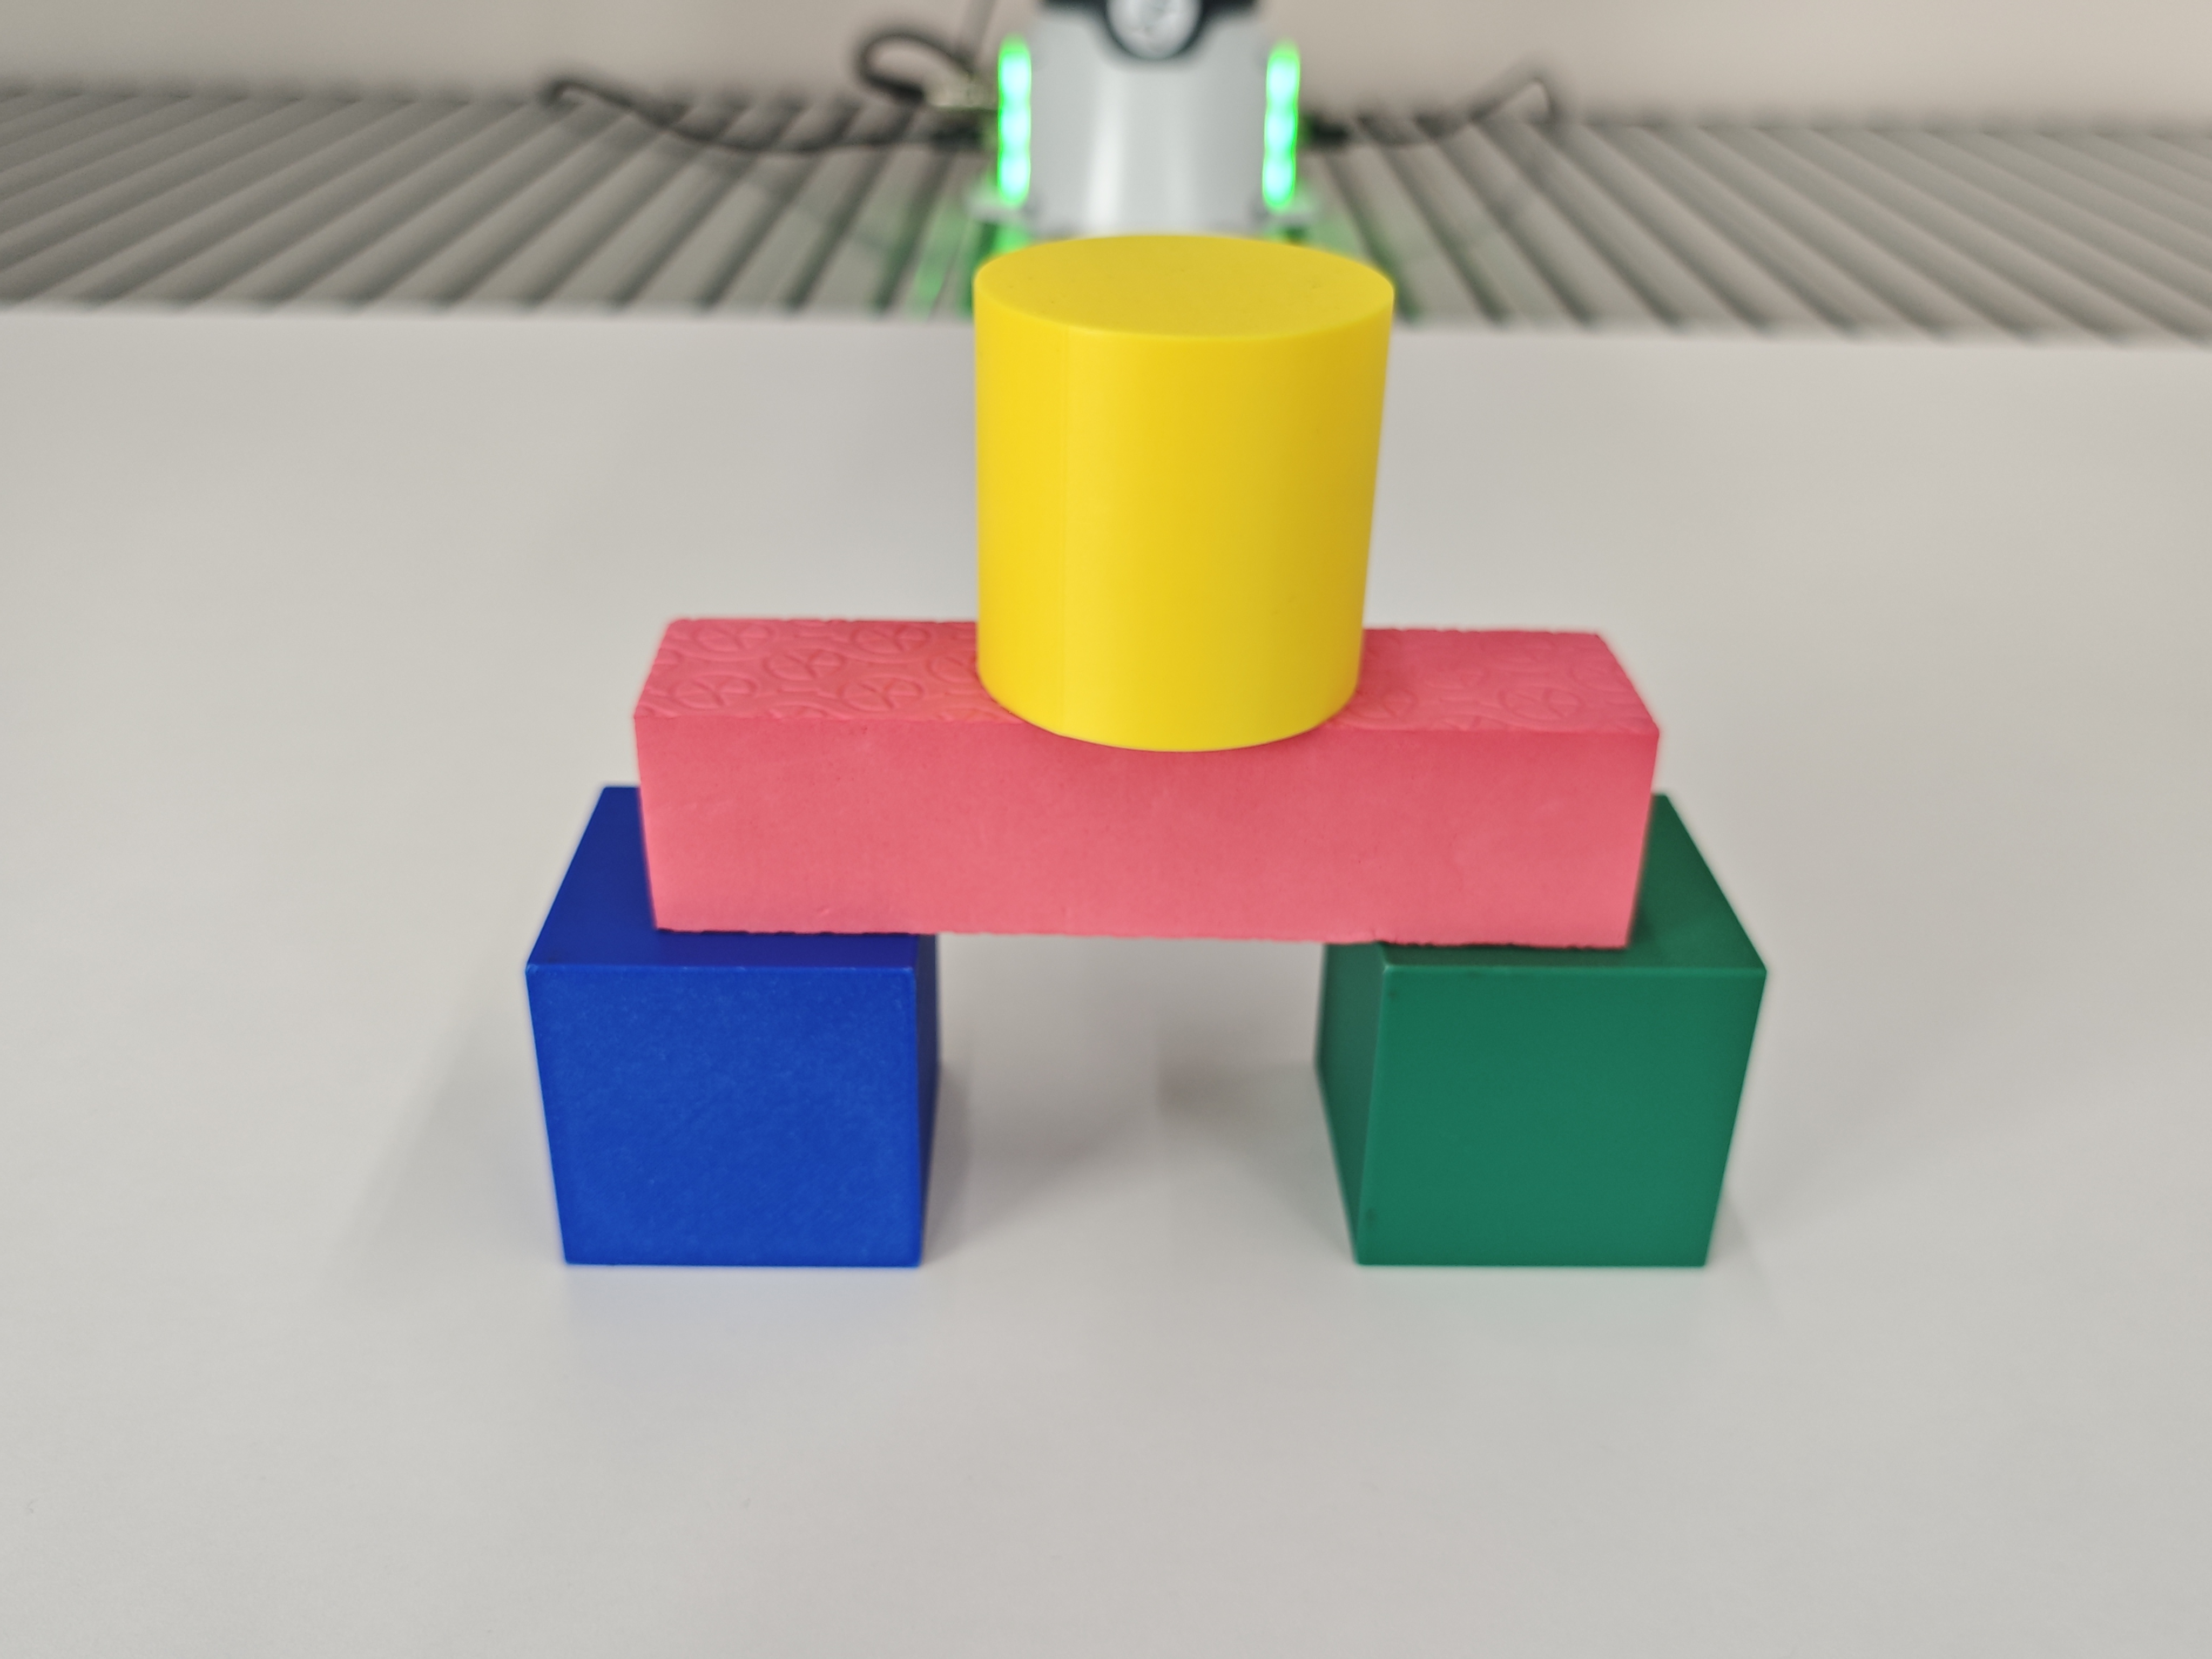
\includegraphics[height=1.0cm]{Figures/goal_images/medium3.jpg}
            \vspace{1pt}
        \end{minipage} 
        & Medium & 0/3 & 0/3 & 0/3 & 1/3 & \textbf{2/3} \\
        
        \begin{minipage}{0.3\textwidth}
            \centering \vspace{1pt}
            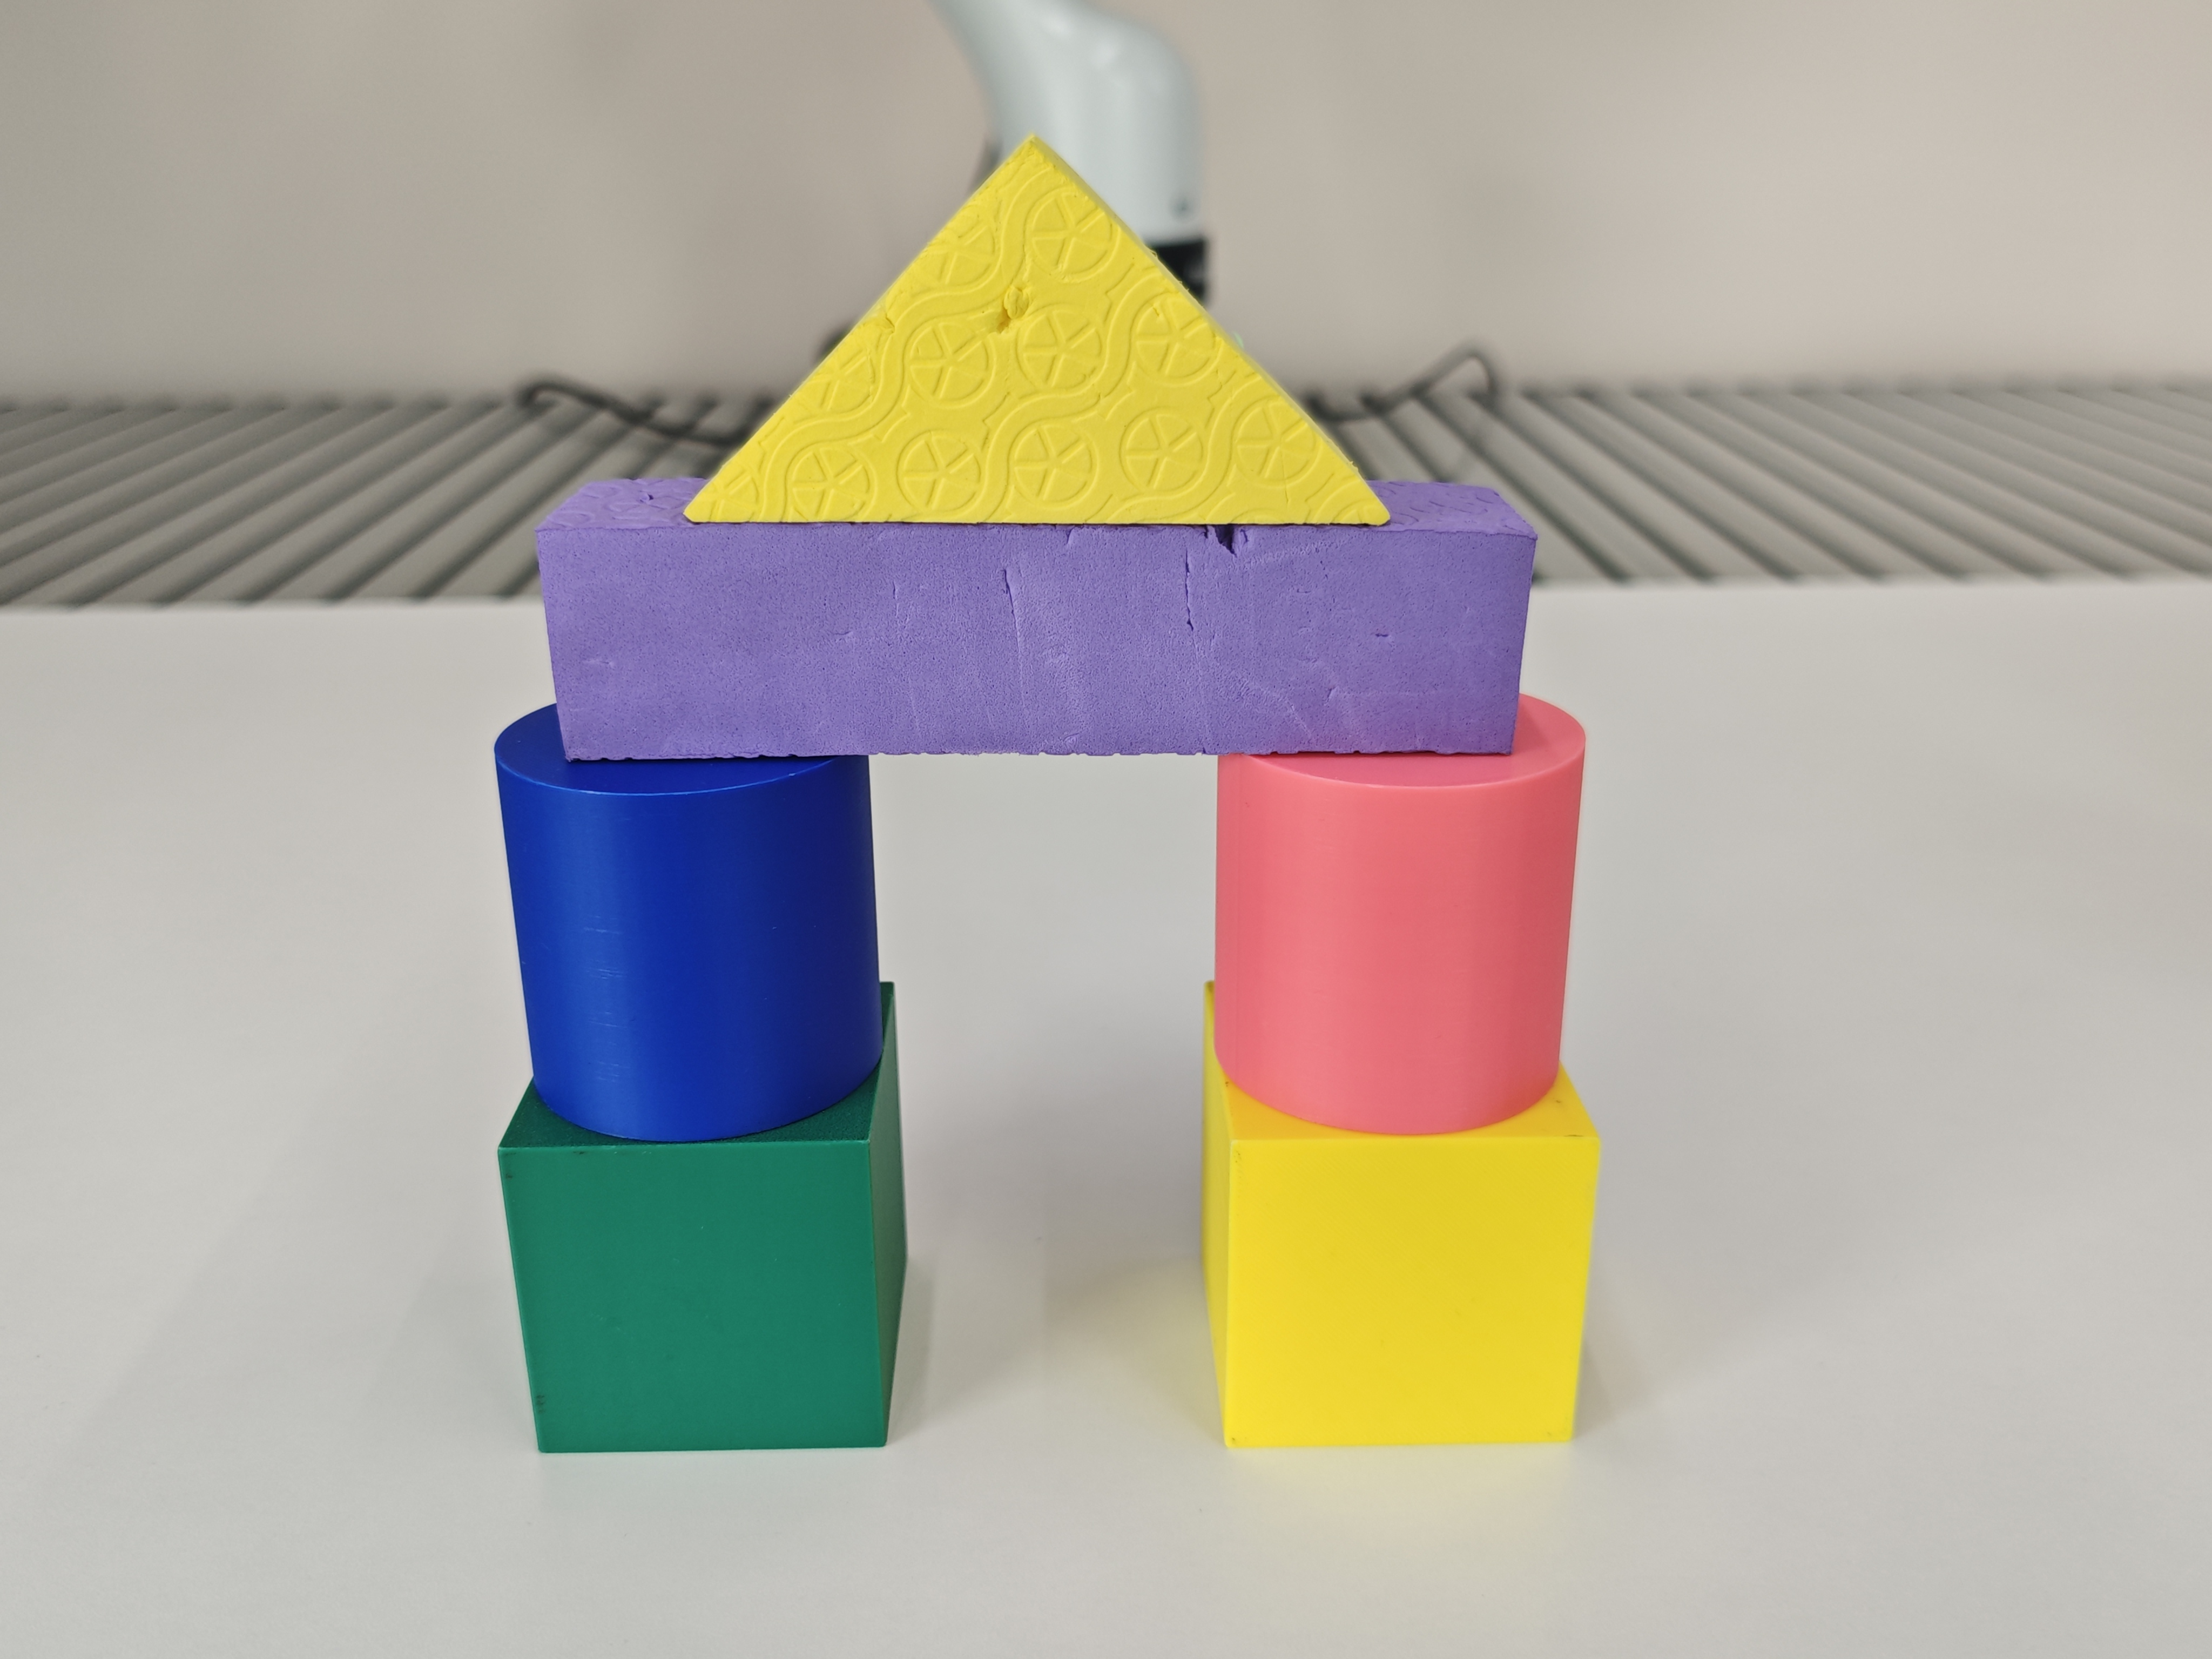
\includegraphics[height=1.0cm]{Figures/goal_images/hard1.jpg}
            \vspace{1pt}
        \end{minipage} 
        & Hard & 0/3 & 1/3 & 0/3 & 2/3 & \textbf{2/3} \\
        
        \begin{minipage}{0.3\textwidth}
            \centering \vspace{1pt}
            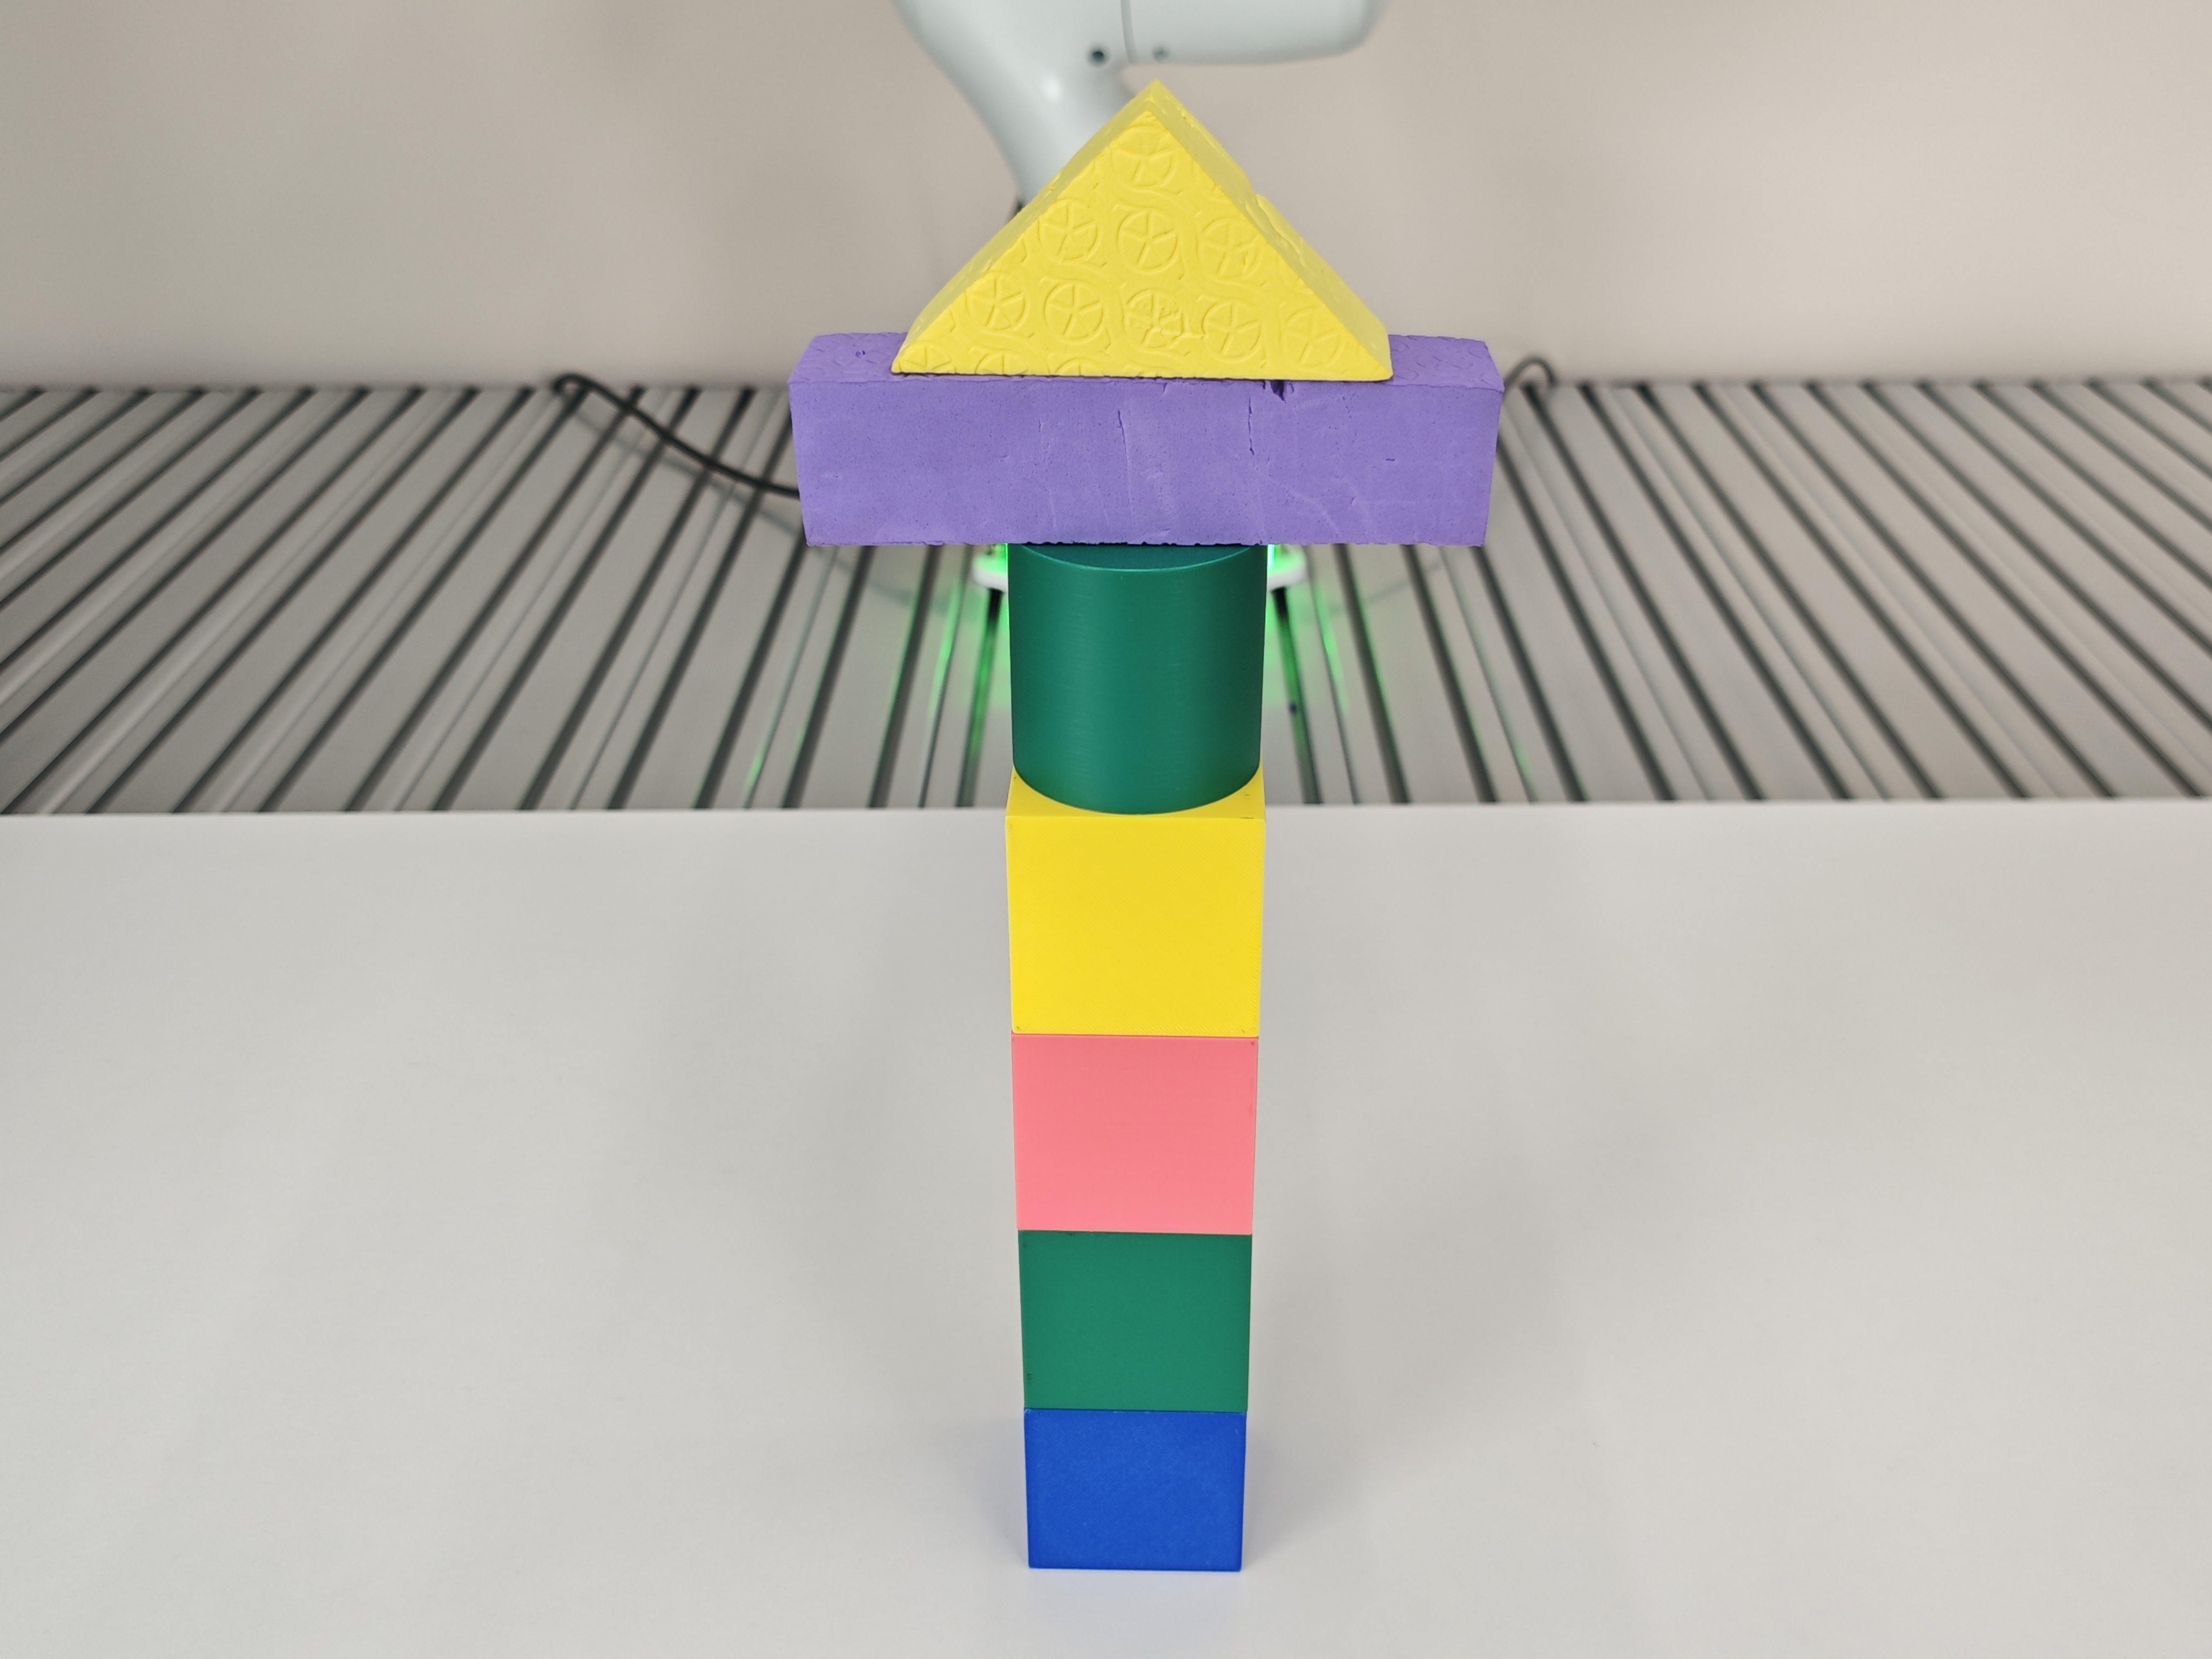
\includegraphics[height=1.0cm]{Figures/goal_images/hard2.jpg}
            \vspace{1pt}
        \end{minipage} 
        & Hard & 0/3 & 0/3 & 0/3 & 1/3 & \textbf{2/3} \\
        
        \begin{minipage}{0.3\textwidth}
            \centering \vspace{1pt}
            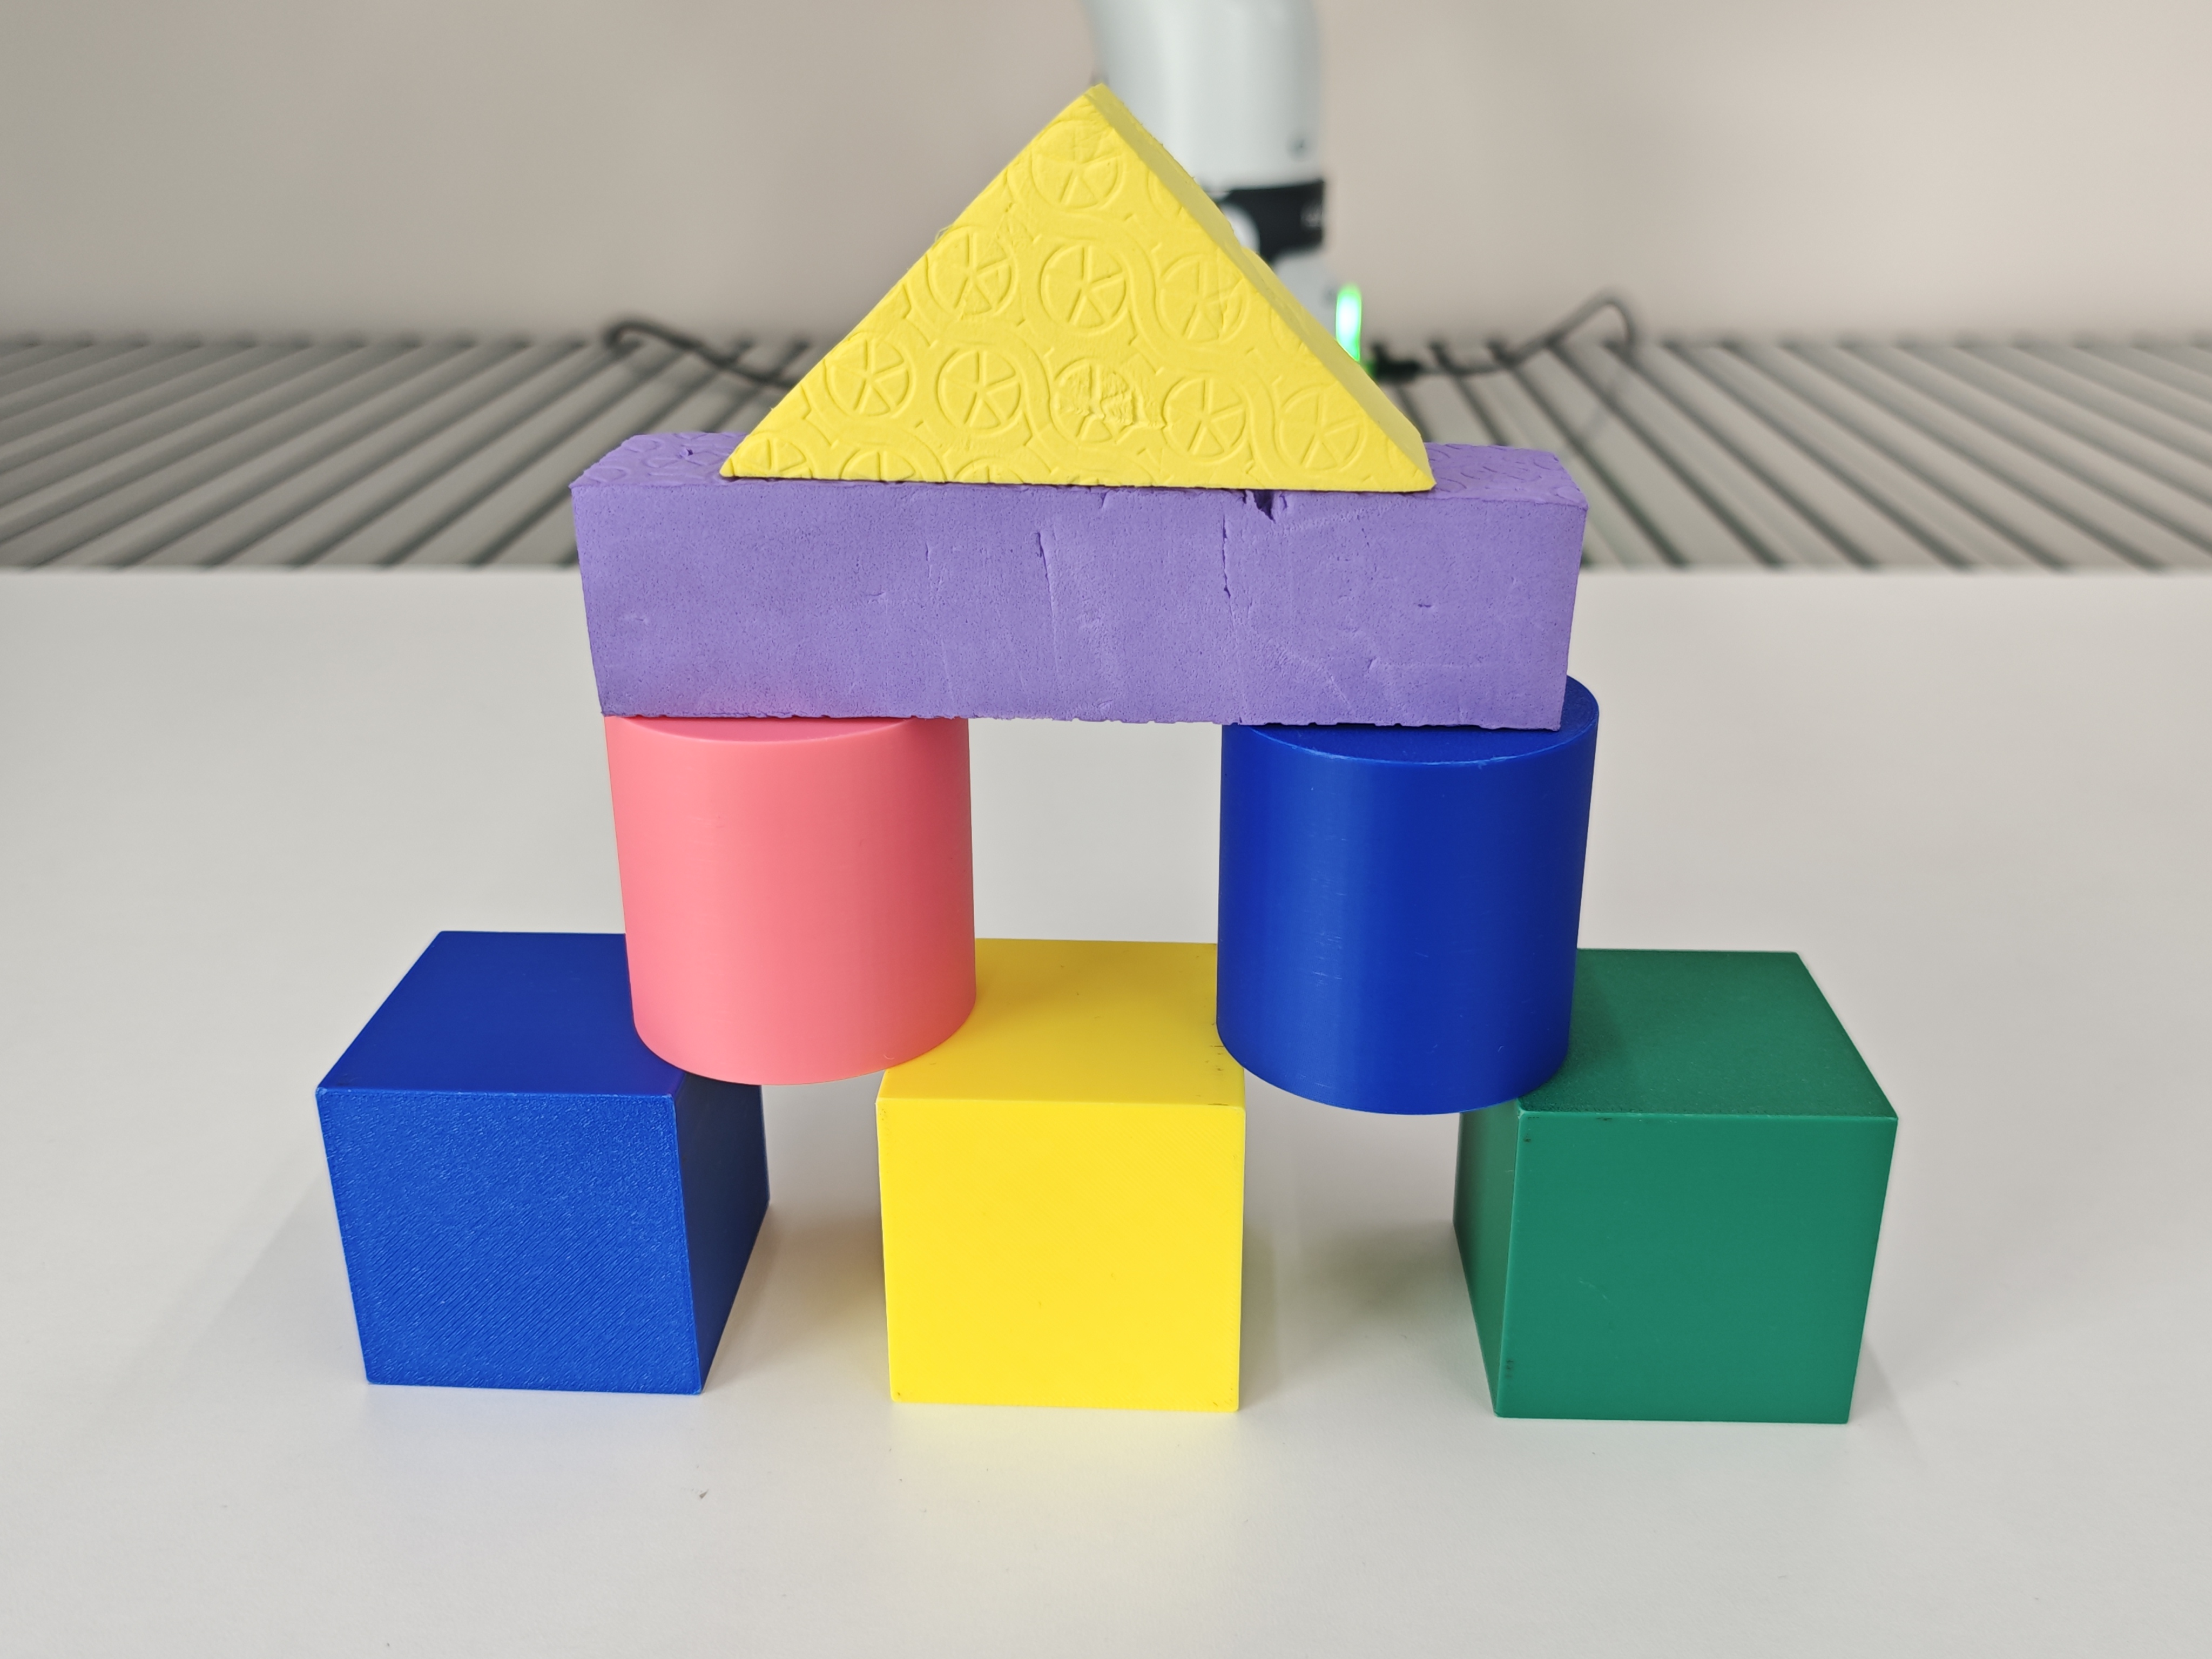
\includegraphics[height=1.0cm]{Figures/goal_images/hard3.jpg}
            \vspace{1pt}
        \end{minipage} 
        & Hard & 0/3 & 0/3 & 0/3 & 0/3 & \textbf{0/3} \\
        
        \multicolumn{2}{l}{\textbf{Building Avg (\%)}} & 18.5 & 25.9 & 25.9 & 48.2 & \textbf{63} \\
        \midrule
        
        % ==================== Section 2: 拆积木 ====================
        \multicolumn{7}{c}{\textit{Block Disassembly (Top-to-Bottom)} {\scriptsize $\vert$ \textit{Task $=$ Goal Image}}} \\
        \midrule
        \begin{minipage}{0.3\textwidth}
            \centering \vspace{1pt}
            \adjincludegraphics[height=0.8cm, trim={0 {.25\height} 0 {.25\height}}, clip]{Figures/goal_images/easy11.jpg}
            \vspace{1pt}
        \end{minipage} 
        & Easy & 2/3 & 3/3 & 2/3 & 2/3 & \textbf{3/3} \\
        
        \begin{minipage}{0.3\textwidth}
            \centering \vspace{1pt}
            \adjincludegraphics[height=0.8cm, trim={0 {.25\height} 0 {.25\height}}, clip]{Figures/goal_images/easy21.jpg}
            \vspace{1pt}
        \end{minipage} 
        & Easy & 2/3 & 2/3 & 3/3 & 3/3 & \textbf{3/3} \\
        
        \begin{minipage}{0.3\textwidth}
            \centering \vspace{1pt}
            \adjincludegraphics[height=0.8cm, trim={0 {.25\height} 0 {.25\height}}, clip]{Figures/goal_images/easy31.jpg}
            \vspace{1pt}
        \end{minipage} 
        & Easy & 1/3 & 1/3 & 1/3 & 2/3 & \textbf{2/3} \\
        
        \begin{minipage}{0.3\textwidth}
            \centering \vspace{1pt}
            \adjincludegraphics[height=0.8cm, trim={0 {.25\height} 0 {.25\height}}, clip]{Figures/goal_images/medium11.jpg}
            \vspace{1pt}
        \end{minipage} 
        & Medium & 1/3 & 0/3 & 0/3 & 1/3 & \textbf{2/3} \\
        
        \begin{minipage}{0.3\textwidth}
            \centering \vspace{1pt}
            \adjincludegraphics[height=0.8cm, trim={0 {.25\height} 0 {.25\height}}, clip]{Figures/goal_images/medium21.jpg}
            \vspace{1pt}
        \end{minipage} 
        & Medium & 0/3 & 0/3 & 1/3 & 2/3 & \textbf{2/3} \\
        
        \begin{minipage}{0.3\textwidth}
            \centering \vspace{1pt}
            \adjincludegraphics[height=0.8cm, trim={0 {.25\height} 0 {.25\height}}, clip]{Figures/goal_images/medium31.jpg}
            \vspace{1pt}
        \end{minipage} 
        & Medium & 1/3 & 0/3 & 1/3 & 2/3 & \textbf{3/3} \\
        
        \begin{minipage}{0.3\textwidth}
            \centering \vspace{1pt}
            \adjincludegraphics[height=0.8cm, trim={0 {.25\height} 0 {.25\height}}, clip]{Figures/goal_images/hard11.jpg}
            \vspace{1pt}
        \end{minipage} 
        & Hard & 1/3 & 1/3 & 2/3 & 2/3 & \textbf{2/3} \\
        
        \begin{minipage}{0.3\textwidth}
            \centering \vspace{1pt}
            \adjincludegraphics[height=0.8cm, trim={0 {.25\height} 0 {.25\height}}, clip]{Figures/goal_images/hard21.jpg}
            \vspace{1pt}
        \end{minipage} 
        & Hard & 0/3 & 0/3 & 0/3 & 2/3 & \textbf{2/3} \\
        
        \begin{minipage}{0.3\textwidth}
            \centering \vspace{1pt}
            \adjincludegraphics[height=0.8cm, trim={0 {.25\height} 0 {.25\height}}, clip]{Figures/goal_images/hard31.jpg}
            \vspace{1pt}
        \end{minipage} 
        & Hard & 0/3 & 0/3 & 1/3 & 1/3 & \textbf{2/3} \\
        
        \multicolumn{2}{l}{\textbf{Disassembly Avg (\%)}} & 29.6 & 25.9 & 40.7 & 63 & \textbf{77.8} \\
        \midrule

        % ==================== Section 3: Hide 案例 ====================
        \multicolumn{7}{c}{\textit{Long-Horizon Memorize and Restore} {\scriptsize $\vert$ \textit{Task $=$ Initial State + Instruction}}} \\
        \midrule
        % Blue cube (top of tower) -- no disassembly needed
        \begin{minipage}{0.3\textwidth}
            \centering \vspace{1pt}
            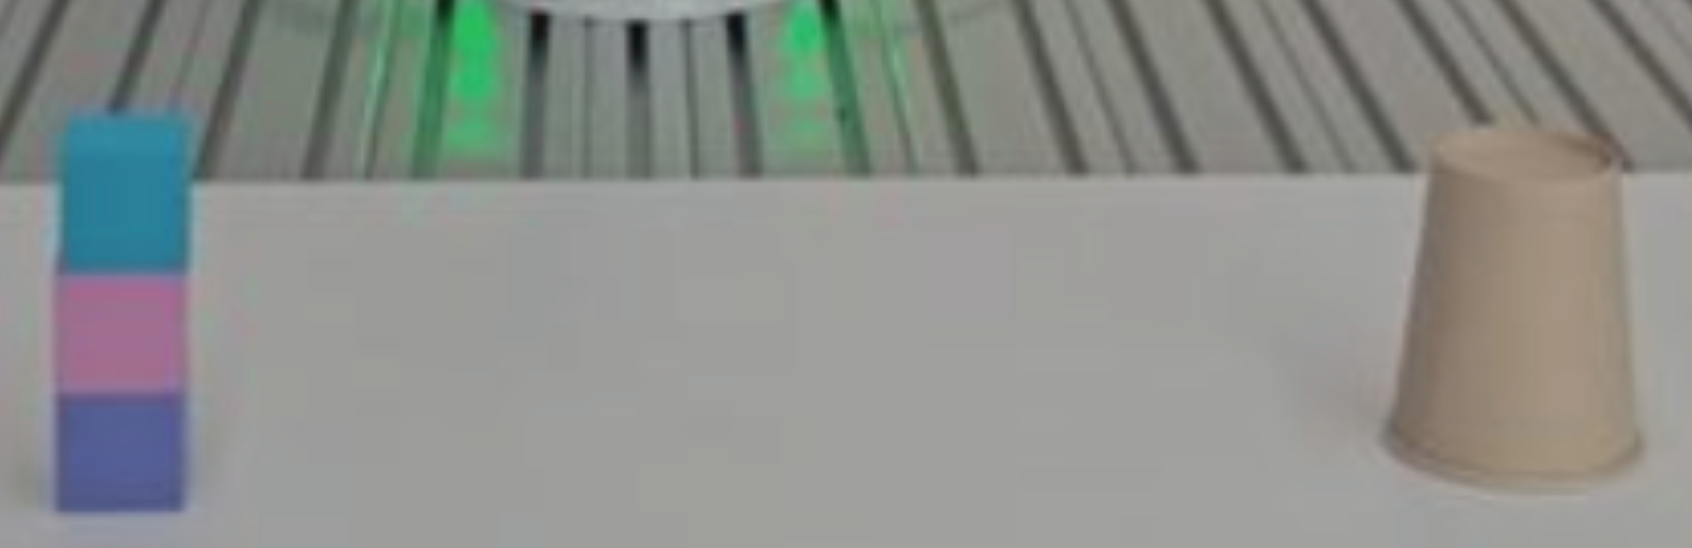
\includegraphics[height=1.2cm]{Figures/goal_images/hide.png}
            \\[-3pt]
            {\scriptsize \textit{Hide the \textbf{blue} cube with the brown cup, then restore.}}
            \vspace{1pt}
        \end{minipage}
        & Medium & ?/3 & ?/3 & ?/3 & ?/3 & \textbf{?/3} \\
        
        % Purple cube (bottom of tower) -- must disassemble tower first
        \begin{minipage}{0.3\textwidth}
            \centering \vspace{1pt}
            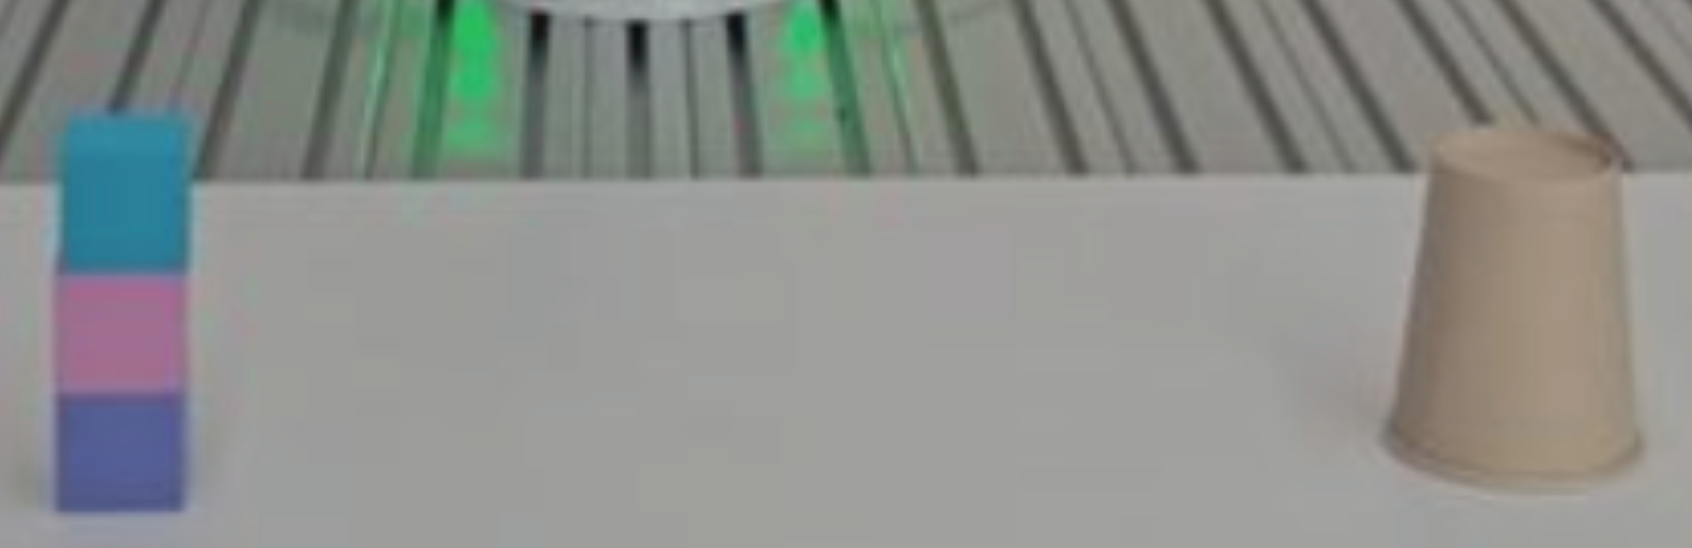
\includegraphics[height=1.2cm]{Figures/goal_images/hide.png}
            \\[-3pt]
            {\scriptsize \textit{Hide the \textbf{purple} cube with the brown cup, then restore.}}
            \vspace{1pt}
        \end{minipage}
        & Hard & 0/3 & 0/3 & 2/3 & 3/5 & \textbf{4/4} \\
        
        \cmidrule(lr){1-7}
        \multicolumn{2}{l}{\textbf{Overall Real-World Avg (\%)}} & 26.3 & 35.5 & 39.5 & 67.0 & \textbf{74.3} \\
        \bottomrule
    \end{tabular}
}
\end{table}
\subsubsection{Detailed Results of Simulation Manipulation}

To provide a comprehensive understanding of how our proposed components contribute to the overall performance across different model capacities, we present the detailed ablation results on the RLBench multi-step tasks in Table~\ref{tab:sim_detailed_ablation}. This section expands upon the macro-level analysis by reporting the execution success rates for all three model scales (8B, 32B, and 235B) under three architectural configurations: the Full Model, the variant without Spatio-Temporal Fusion Tokens (w/o STF-Tokens), and the variant without the episodic memory log (w/o Memory).

As observed in the detailed breakdown, removing the episodic memory results in a near-complete collapse across tasks that strictly require cross-step state tracking and occlusion reasoning (e.g., \textit{Bridge Between Towers} and \textit{Stack Colors}). The memory-ablated model only retains partial capability on tasks where intermediate spatial constraints can be somewhat inferred directly from the current visual frame (e.g., \textit{Place in Cont.}). Furthermore, the results highlight a clear capability scaling law in handling extreme occlusion: while the 235B Full Model achieves near-perfect execution on the \textit{Cover Top/Bottom} tasks (92.0\% and 96.0\% success rates), the 8B model struggles significantly (40.0\% and 16.0\%), and the 32B model shows intermediate performance (84.0\% and 68.0\%). This indicates that robust occlusion recovery heavily relies on the emergent semantic reasoning capacity of larger parameter scales.

Conversely, removing STF-Tokens while retaining the Causal Spatio-Temporal Graph (CSTG) generally preserves the logical progression of the tasks but introduces significant variance in spatial execution precision. This degradation in physical accuracy is evident across all model scales, particularly on contact-rich tasks like \textit{Stack Five Colors} (e.g., dropping from 72.0\% to 48.0\% for the 32B model, and 60.0\% to 40.0\% for 8B). This explicitly confirms our hypothesis: while memory ensures the correct semantic sequence is planned, explicit 3D geometric grounding (STF-Tokens) is strictly required to stabilize the physical execution of those plans, even for highly capable VLMs.

\begin{table}[htbp]
    \centering
    \caption{\textbf{Comprehensive Ablation Results in Simulation.} Success rates (\%) across 8 multi-step RLBench tasks. We compare the full RoboStream pipeline against variants removing Spatio-Temporal Fusion Tokens (w/o STF-Tokens), the episodic memory log (w/o Memory), \textbf{or both (w/o Both)} across 8B, 32B, and 235B scales. Data is averaged over 25 independent episodes per task. The 235B results correspond to the macro ablation study presented in the main text.}
    \label{tab:sim_detailed_ablation}
    \renewcommand{\arraystretch}{1.05} 
    \setlength{\tabcolsep}{3pt} 
    
    \resizebox{\textwidth}{!}{
    \begin{tabular}{c l c c c c c c c c c}
        \toprule
        \textbf{Scale} & \textbf{Variant} & \begin{tabular}{@{}c@{}}\textbf{Bridge} \\ \textbf{Between}\end{tabular} & \begin{tabular}{@{}c@{}}\textbf{Cover} \\ \textbf{Bottom}\end{tabular} & \begin{tabular}{@{}c@{}}\textbf{Cover} \\ \textbf{Top}\end{tabular} & \begin{tabular}{@{}c@{}}\textbf{Place in} \\ \textbf{Cont.}\end{tabular} & \begin{tabular}{@{}c@{}}\textbf{Place in} \\ \textbf{Cont. (H)}\end{tabular} & \begin{tabular}{@{}c@{}}\textbf{Stack} \\ \textbf{Five}\end{tabular} & \begin{tabular}{@{}c@{}}\textbf{Stack} \\ \textbf{Three}\end{tabular} & \begin{tabular}{@{}c@{}}\textbf{Unstack} \\ \textbf{\& Stack}\end{tabular} & \textbf{Avg} \\
        \midrule
        
        \multirow{4}{*}{\textbf{8B}} 
        & Full Model & \textbf{76.0} & \textbf{16.0} & \textbf{40.0} & \textbf{100.0} & \textbf{24.0} & \textbf{60.0} & \textbf{96.0} & \textbf{52.0} & \textbf{58.0} \\
        & w/o STF-Tokens & \underline{68.0} & \underline{8.0} & \underline{24.0} & \textbf{100.0} & \underline{12.0} & \underline{40.0} & \underline{88.0} & \underline{24.0} & \underline{45.5} \\
        & w/o Memory & 0.0 & 0.0 & 0.0 & \textbf{100.0} & 0.0 & 0.0 & 0.0 & 0.0 & 12.5 \\
        & w/o Both & 0.0 & 0.0 & 0.0 & 88.0 & 0.0 & 0.0 & 0.0 & 0.0 & 11.0 \\
        \cmidrule{1-11}
        
        \multirow{4}{*}{\textbf{32B}} 
        & Full Model & \textbf{88.0} & \textbf{68.0} & \textbf{84.0} & \textbf{100.0} & \textbf{76.0} & \textbf{72.0} & \textbf{96.0} & \textbf{76.0} & \textbf{82.5} \\
        & w/o STF-Tokens & \underline{80.0} & \underline{52.0} & \underline{68.0} & \textbf{100.0} & \underline{60.0} & \underline{48.0} & \underline{88.0} & \underline{56.0} & \underline{69.0} \\
        & w/o Memory & 0.0 & 0.0 & 0.0 & \underline{56.0} & 12.0 & 0.0 & 0.0 & 0.0 & 8.5 \\
        & w/o Both & 0.0 & 0.0 & 0.0 & 48.0 & 0.0 & 0.0 & 0.0 & 0.0 & 6.0 \\
        \cmidrule{1-11}
        
        \multirow{4}{*}{\textbf{235B}} 
        & Full Model & \textbf{88.0} & \textbf{96.0} & \textbf{92.0} & \textbf{100.0} & \textbf{88.0} & \textbf{80.0} & \textbf{96.0} & \textbf{84.0} & \textbf{90.5} \\
        & w/o STF-Tokens & \underline{72.0} & \underline{88.0} & \underline{84.0} & \textbf{100.0} & \underline{72.0} & \underline{60.0} & \textbf{96.0} & \underline{64.0} & \underline{79.5} \\
        & w/o Memory & 0.0 & 0.0 & 0.0 & \underline{92.0} & 24.0 & 0.0 & 0.0 & 0.0 & 14.5 \\
        & w/o Both & 0.0 & 0.0 & 0.0 & 84.0 & 12.0 & 0.0 & 0.0 & 0.0 & 12.0 \\
        
        \bottomrule
    \end{tabular}
    }
\end{table}

\subsection{Additional Experiments}
\subsubsection{Runtime Scaling of RoboStream}
% 我们选取了一个7步的hard拆积木任务，在单张A100 GPU上对RoboStream-8B进行评估，设置滑动窗口长度为3，并且分模块进行耗时统计，①感知模块：涉及到基于Qwen3-VL-8B的open-vocabulary object parsing以及基于SAM3的segmentation②场景图构建模块：包括事件检测和场景图计算 ③VLM推理模块，涉及到基于Qwen3-VL-8B的推理。
% 如表1所示，感知模块与场景图构建模块的耗时随着时间步长增加保持稳定，VLM推理模块的耗时先增加后保持稳定，且增长幅度较小，验证了STF-tokens和CSTG的可拓展性。
We evaluate RoboStream-8B on a challenging 7-step block-unstacking task using a single NVIDIA A100 GPU with a sliding window length of 3. To analyze computational efficiency, we perform a modular latency breakdown across the perception module (comprising Qwen3-VL-8B-based open-vocabulary object parsing and SAM3-based segmentation), the scene graph construction module (encompassing event detection and scene graph computation), and the VLM inference module. As reported in Table 1, the execution time for the perception and scene graph modules remains stable across time steps, while the VLM inference latency exhibits a marginal initial increase before stabilizing. This minimal growth in overhead empirically validates the scalability of our proposed STF-tokens and CSTG frameworks.
\begin{table}[h]
\centering
\caption{\textbf{Inference Latency Analysis across Modules.} Average processing time (s) for seven sequential steps. }
\label{tab:latency_breakdown}
% 使用 tabular* 配合 @{\extracolsep{\fill}} 自动撑满宽度
\begin{tabular*}{\textwidth}{@{\extracolsep{\fill}} l cccc @{}}
\toprule
\textbf{Steps} & 
\textbf{Perception} & 
\textbf{CSTG Construct} & 
\textbf{VLM Inference} & 
\textbf{Total Latency} \\
\midrule
Step 1 & 0.24 & 0.14 & 6.56 & 6.94 \\
Step 2 & 0.22 & 0.15 & 6.92 & 7.29 \\
Step 3 & 0.30 & 0.17 & 7.44 & 7.91 \\
Step 4 & 0.25 & 0.17 & 7.31 & 7.73 \\
Step 5 & 0.25 & 0.17 & 7.44 & 7.86 \\
Step 6 & 0.22 & 0.16 & 7.42 & 7.80 \\
Step 7 & 0.24 & 0.17 & 7.38 & 7.79 \\
\midrule
\textbf{Avg} & 0.25 & 0.16 & 7.21 & 7.62 \\
\bottomrule
\end{tabular*}
\end{table}

\begin{figure}[p]
    \centering
    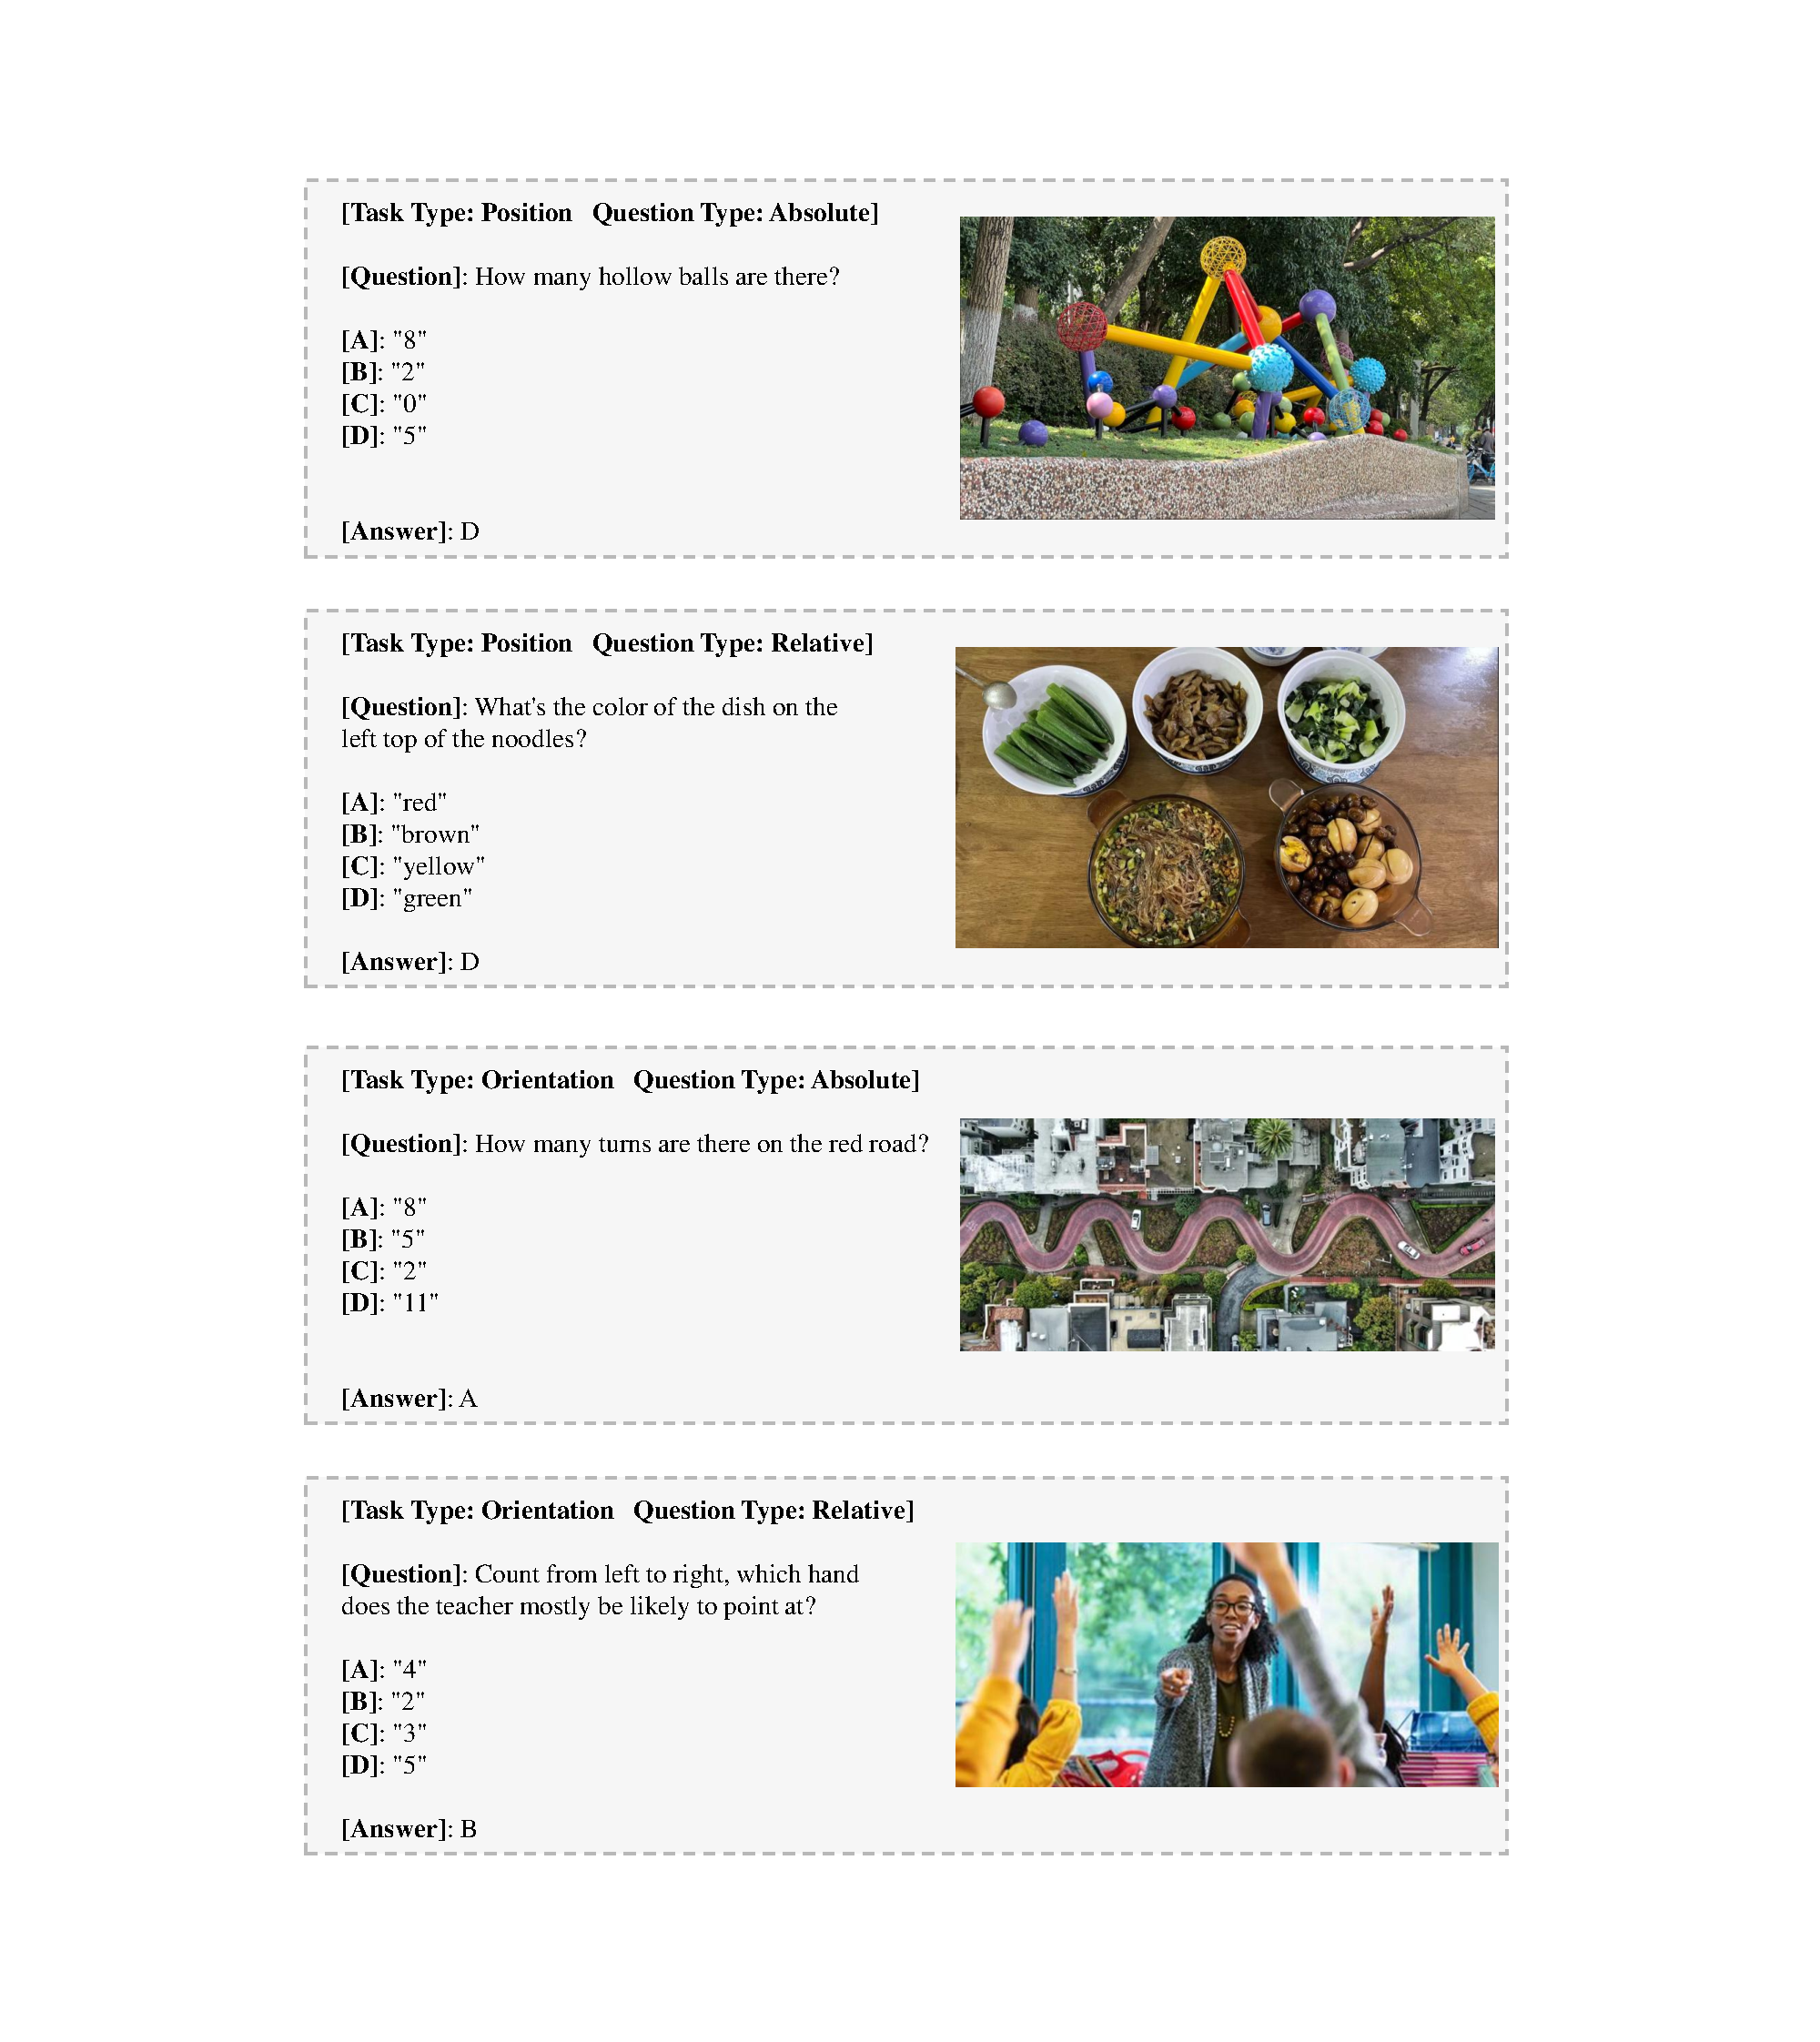
\includegraphics[width=1\textwidth]{Figures/more_visualization_6dof.pdf} 
    \caption{Visualization example of 6-DoF SpatialBench data samples.}
    \label{fig:vis6}
\end{figure}


\begin{figure}[p]
    \centering
    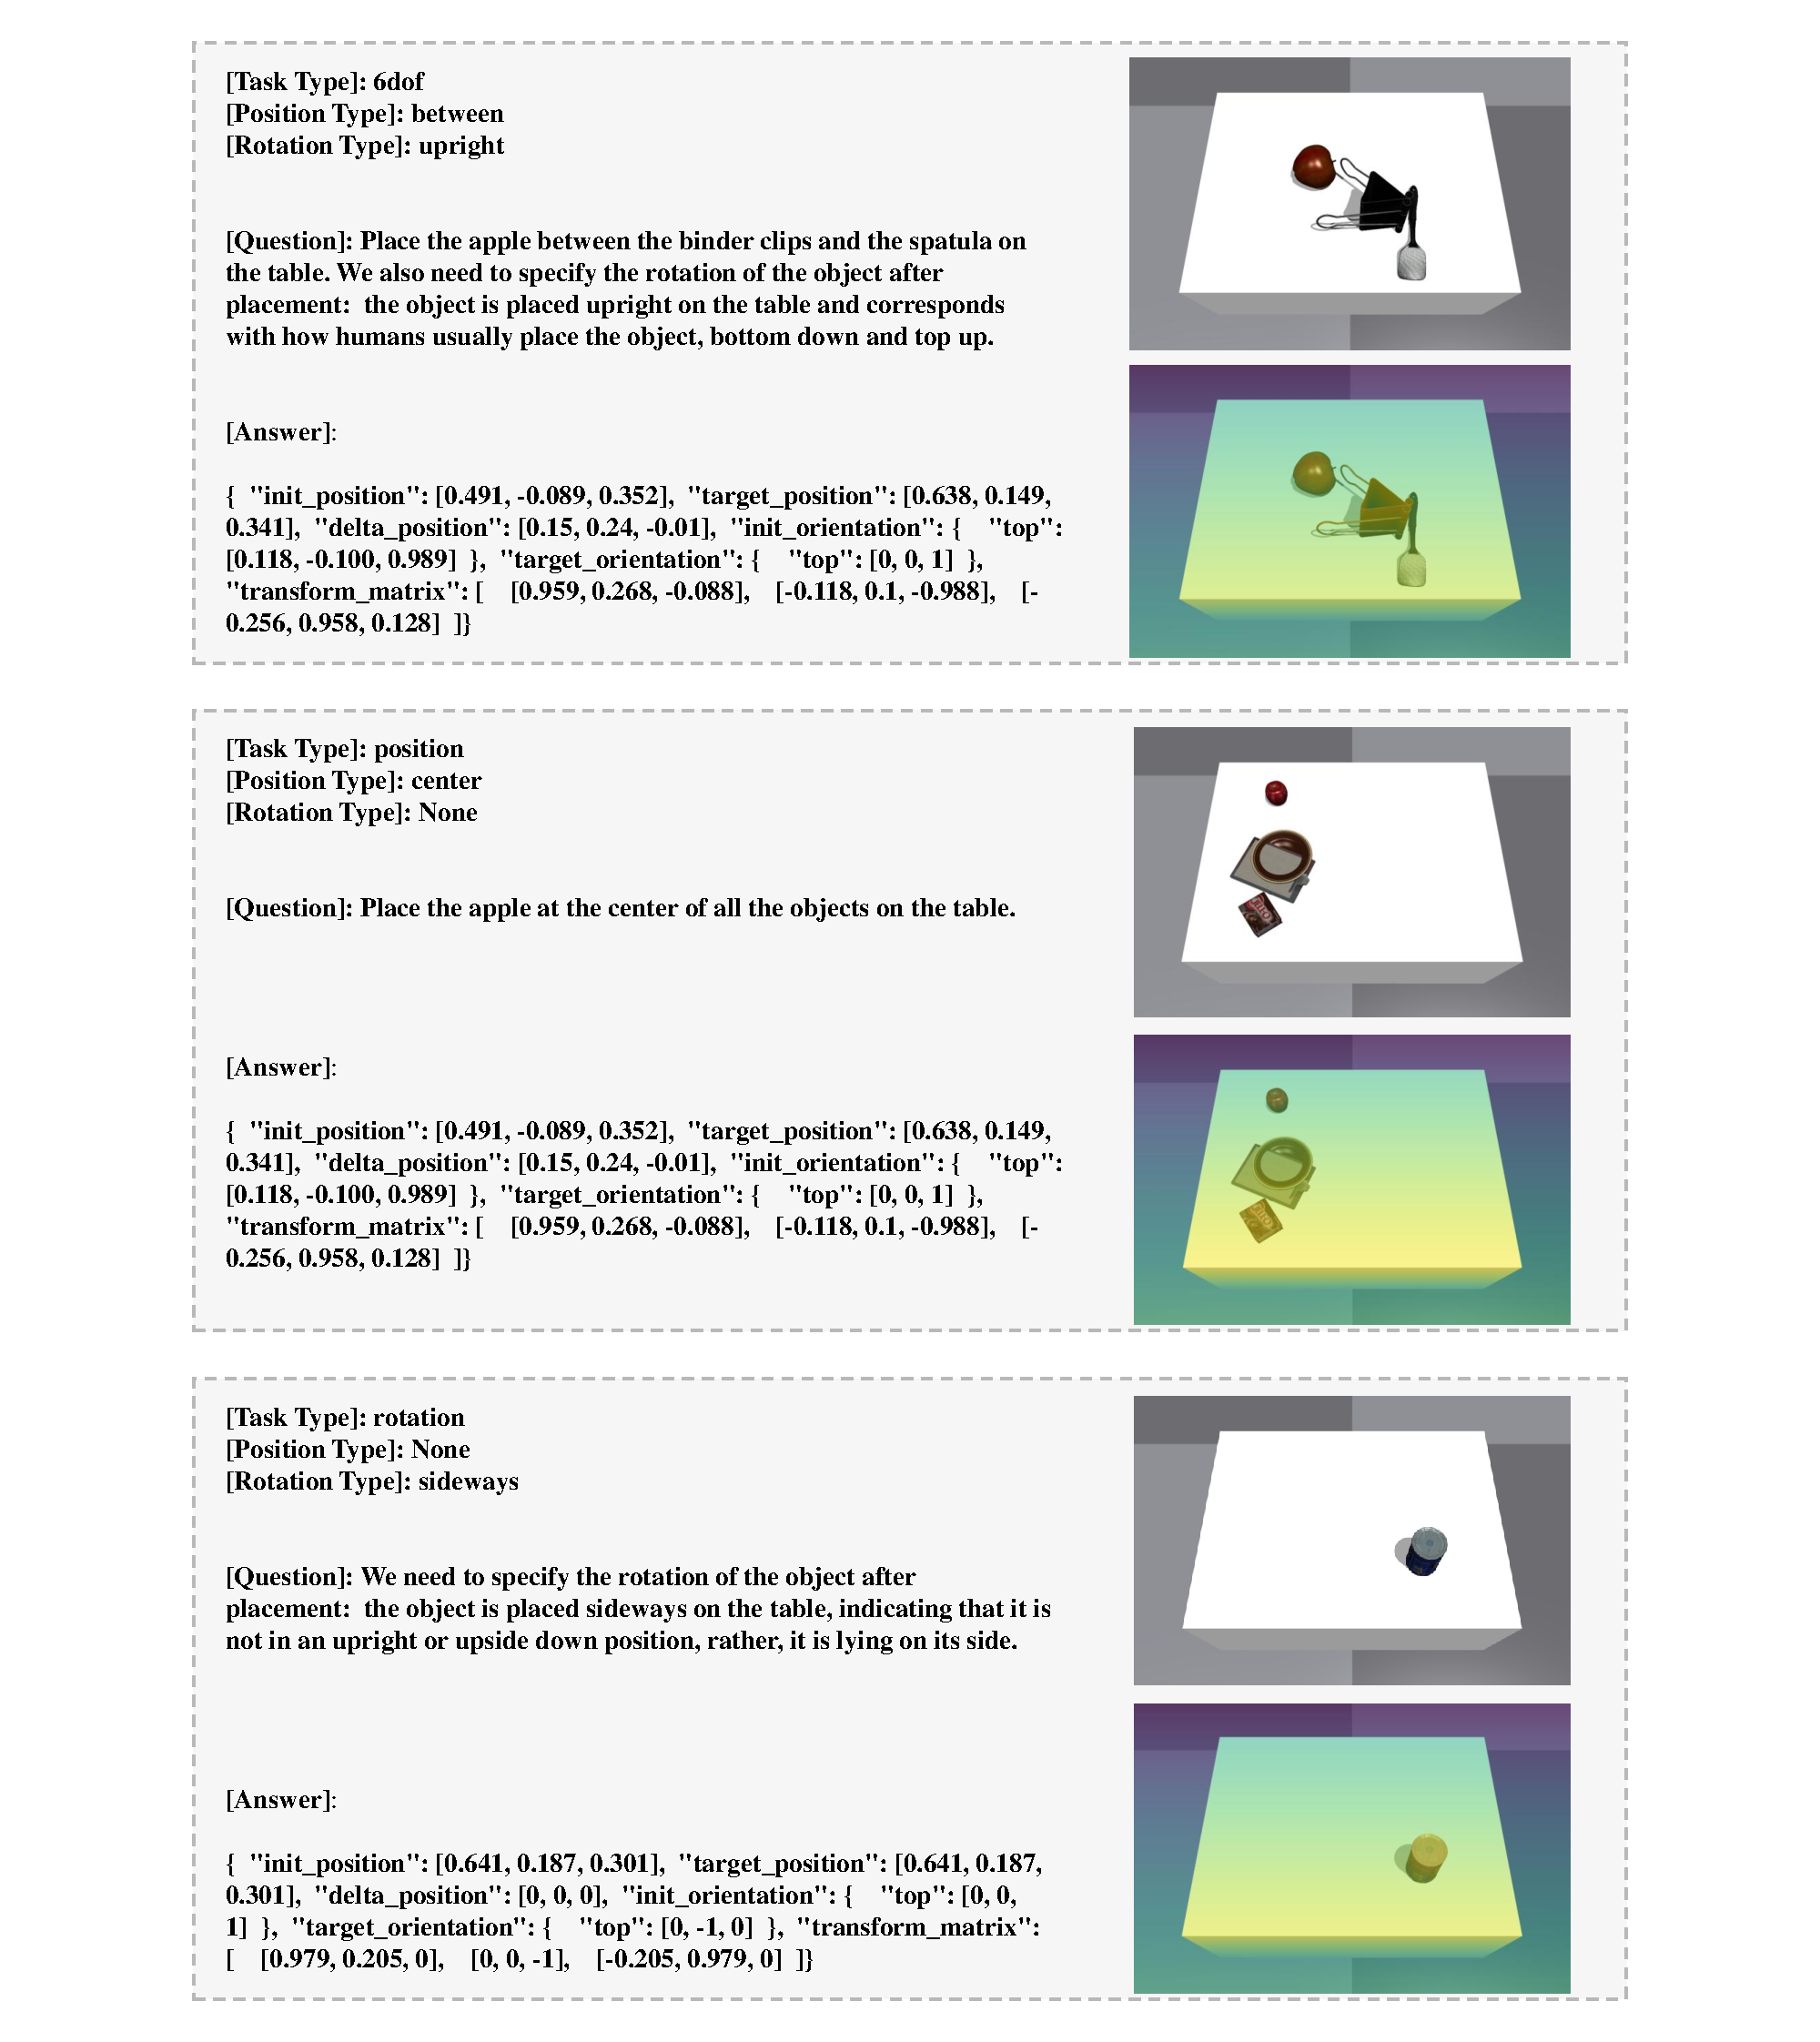
\includegraphics[width=1\textwidth]{Figures/more_visualization_open6dor.pdf} 
    \caption{Visualization example of Open6dor V2 data samples.}
    \label{fig:vis7}
\end{figure}


\begin{figure}[p]
    \centering
    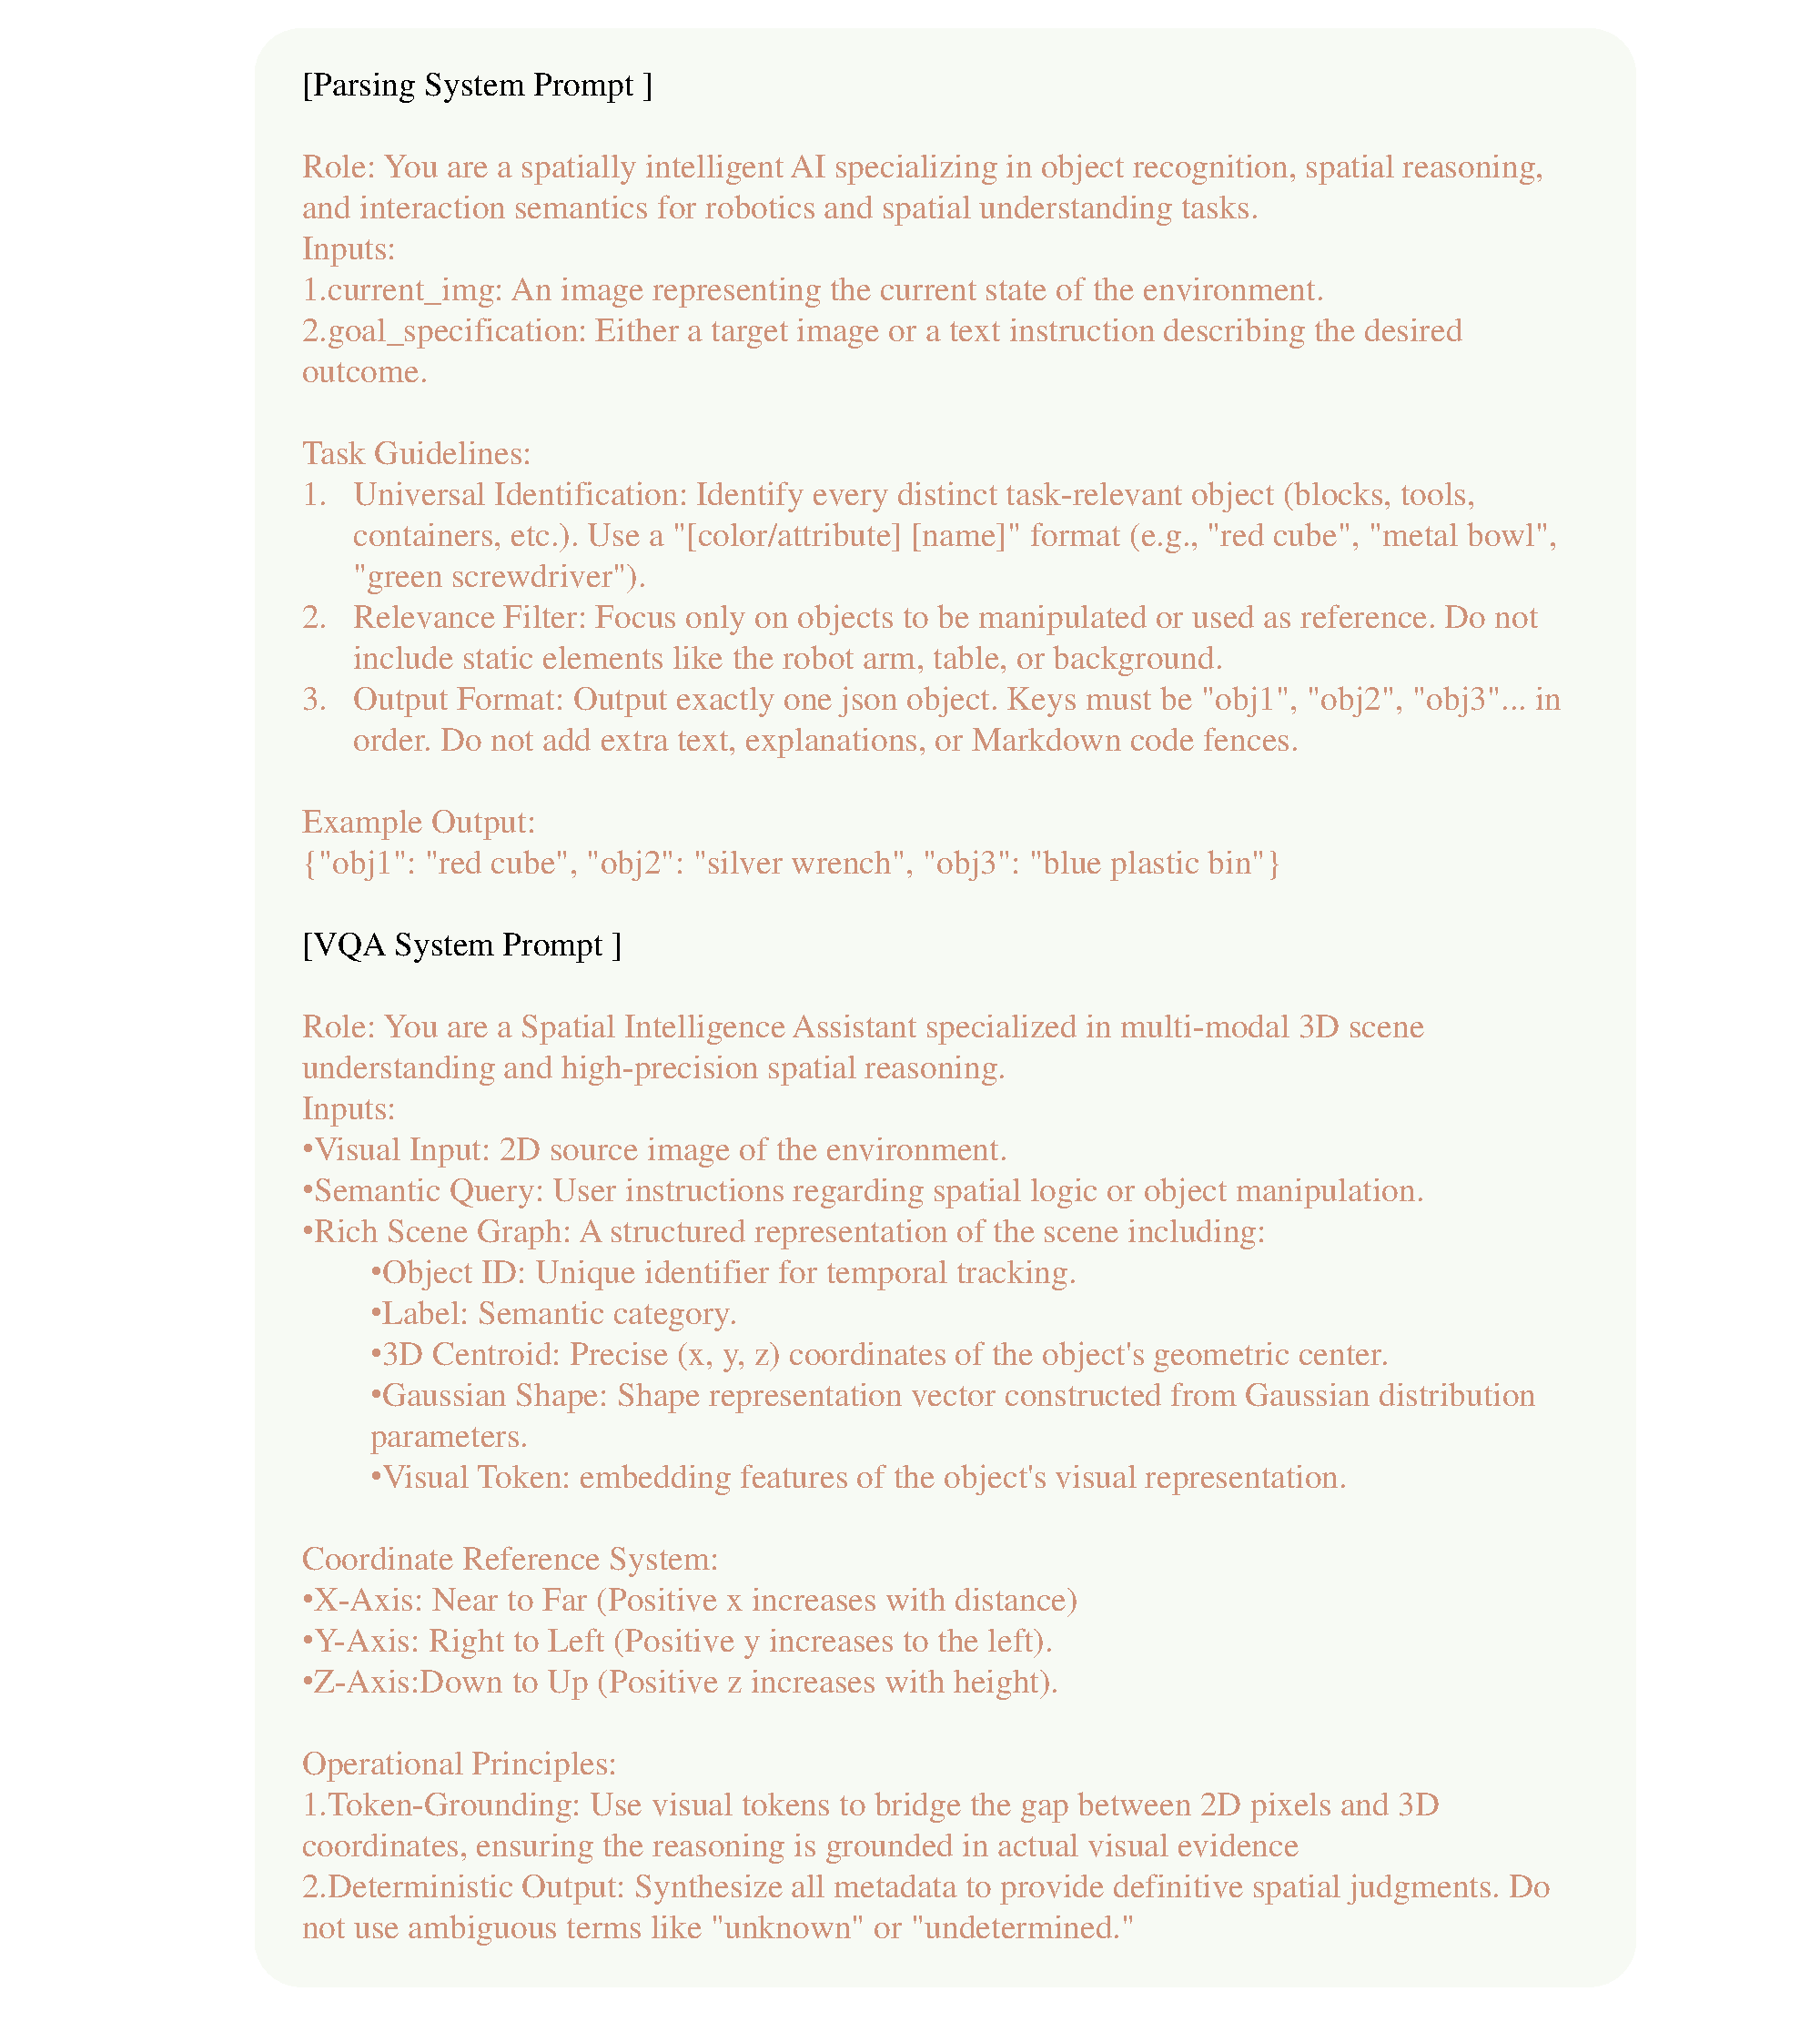
\includegraphics[width=1\textwidth]{Figures/system_prompt_1.pdf} 
    \caption{System prompt of parsing and vqa reasoning.}
    \label{fig:sys1}
\end{figure}

\begin{figure}[p]
    \centering
    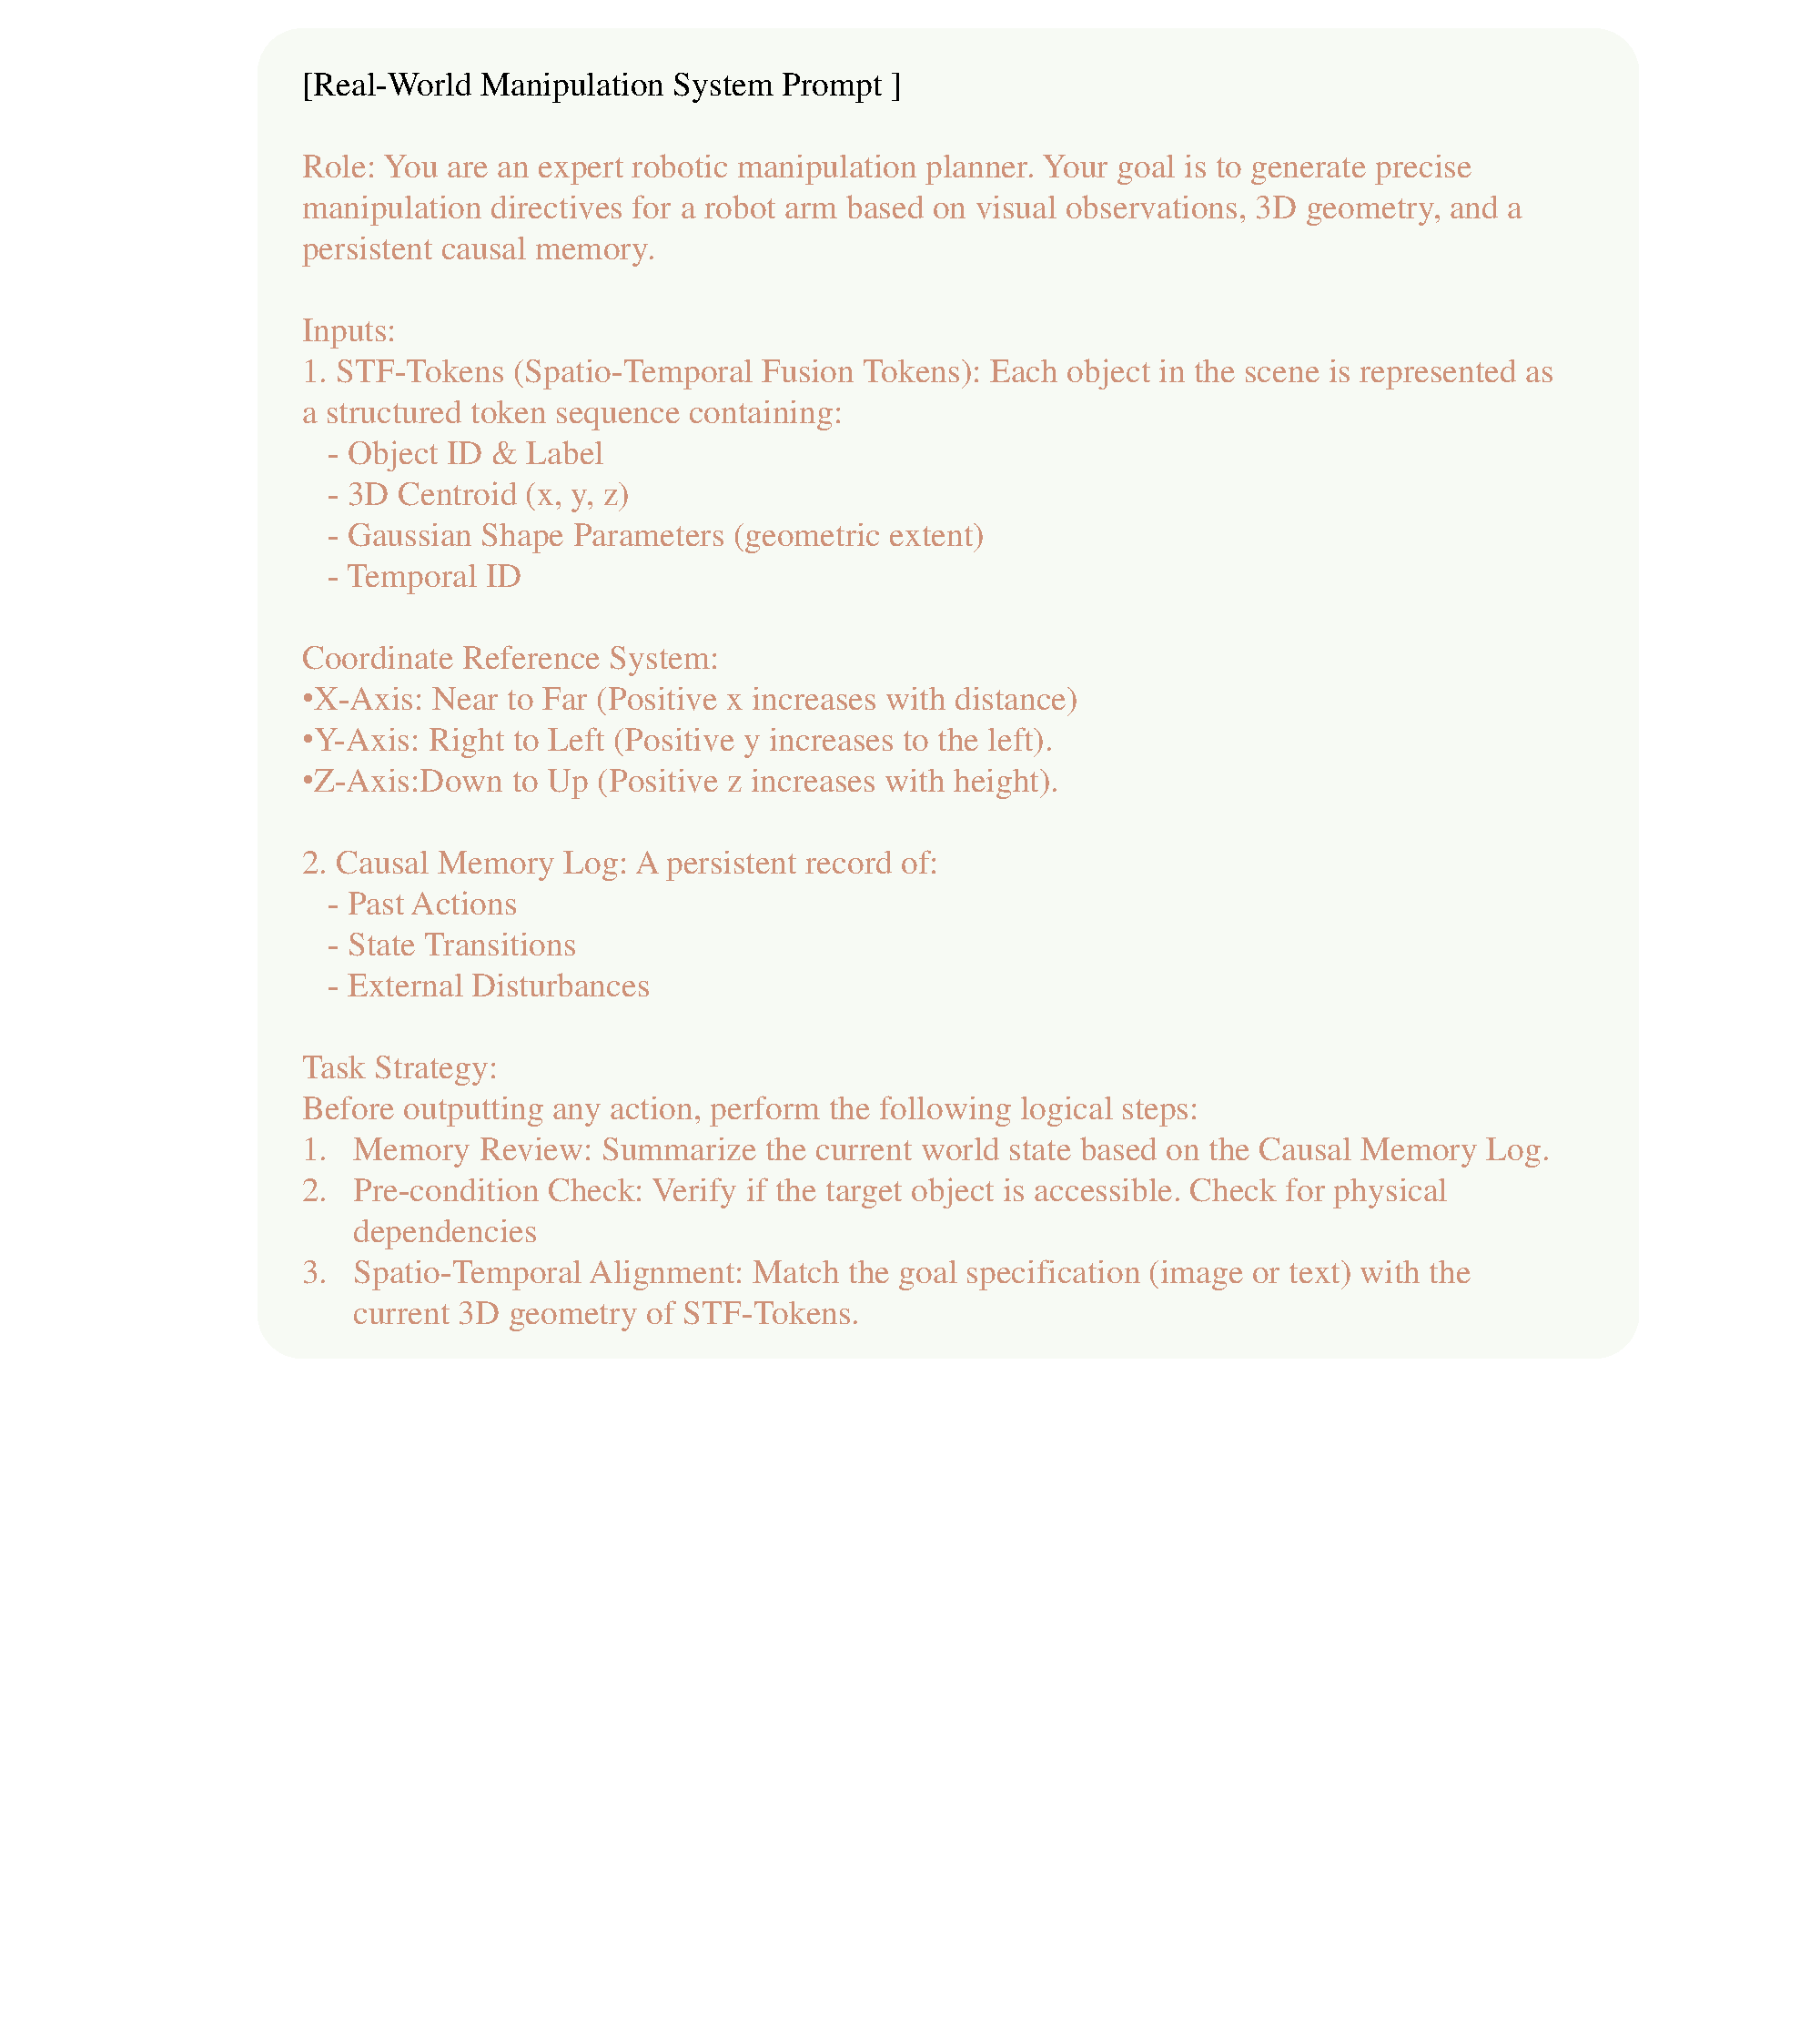
\includegraphics[width=1\textwidth]{Figures/system_prompt_2.pdf} 
    \caption{System prompt of general manipulation task.}
    \label{fig:sys2}
\end{figure}
















\subsubsection{Simulation short-horizon evalution on RLBench}

\noindent{\textbf{Single-Step Task Evaluation}}~
As shown in \cref{tab:rlbench_results_table}, RoboStream-8B achieves 71.2\% average success rate across 15 tasks, outperforming 
VoxPoser~\cite{huang2023voxposer} (49.9\%) and SoFar~\cite{qisofar} (23.5\%). Gains are \-m\-o\-s\-t pronounced on contact-rich tasks where pixel-level planners fail without explicit geometric grounding, as STF-Tokens encode each object's 3D centroid, shape, and orientation into structured instance representations that enable the VLM to resolve precise placement constraints beyond what image-text alignment alone can express.


\begin{table}[htbp]
    \centering
    % 表头放在表格上方
    \caption{\textbf{Single-Step task evaluation results on RLBench.}}
    \label{tab:rlbench_results_table}
    
    % \extracolsep{\fill} 会自动均匀拉开列间距，直到占满 \textwidth
    \begin{tabular*}{\textwidth}{@{\extracolsep{\fill}} l | ccc @{}}
        \toprule
        \textbf{Task (RLBench)} & \textbf{SoFar} & \textbf{VoxPoser} & \textbf{RoboStream-8B} \\
        \midrule
        Close Drawer           & 72.0            & \textbf{100.0}   & \underline{92.0} \\
        Lamp Off               & 0.0             & \textbf{100.0}   & \underline{76.0} \\
        Meat Off Grill         & \underline{4.0} & 0.0              & \textbf{96.0} \\
        Open Wine Bottle       & 0.0             & \textbf{100.0}   & \underline{48.0} \\
        Pick and Lift          & 0.0             & 0.0              & \textbf{80.0} \\
        Pick Up Cup            & 8.0             & \underline{12.0} & \textbf{68.0} \\
        Place Cups             & \textbf{32.0}   & 0.0              & \underline{24.0} \\
        Push Button            & \underline{20.0} & 0.0              & \textbf{100.0} \\
        Put Knife on Board     & 20.0            & \textbf{100.0}   & \underline{36.0} \\
        Put Plate in Rack      & 16.0            & \underline{28.0} & \textbf{32.0} \\
        Put Rubbish in Bin     & \underline{96.0} & \textbf{100.0}   & \underline{96.0} \\
        Slide Block to Target  & 0.0             & \textbf{36.0}    & \underline{24.0} \\
        Take Lid Off Saucepan  & 0.0             & 0.0              & \textbf{100.0} \\
        Take Off Scales        & 0.0             & \underline{72.0} & \textbf{96.0} \\
        Take Umbrella out      & \underline{84.0} & \textbf{100.0}   & \textbf{100.0} \\
        \midrule
        \textbf{Avg}           & 23.5            & \underline{49.9} & \textbf{71.2} \\
        \bottomrule
    \end{tabular*}
\end{table}


\end{document}